\documentclass[../../main.tex]{subfiles}

\setcounter{footnote}{0} 

\newcommand{\cgbind}{\emph{cgbind }}
\newcommand{\MLf}{M$_2$L$_4$ }
\newcommand{\MLs}{M$_4$L$_6$ }
\newcommand{\de}{$\Delta E$}
\newcommand{\dde}{$\Delta\Delta E$}

\NewDocumentCommand{\class}{v}{%
	\texttt{\textcolor{black}{#1}}%
}

\NewDocumentCommand{\code}{v}{%
	\texttt{\textcolor{black}{#1}}%
}

\begin{document}


\section{Manuscript II}
\emph{cgbind: A Python Module and Web App for Automated Metallocage Construction and Host-Guest Characterization}


\subsection{Abstract}

Metallocages offer a diverse and underexplored region of chemical space to search for novel catalysts and substrate hosts. However, the ability to tailor such structures towards applications in binding and catalysis is a challenging task. Here, we present an open-source computational toolkit, \cgbind, that facilitates the construction, characterization and prediction of functional metallocages. It employs known structural scaffolds as starting points and computationally efficient approaches for property evaluation. We demonstrate the ability of \cgbind to construct libraries of cages with varied topologies and linker functionalities, generate accurate geometries (RMSD $<$1.5 Å to crystal structures) and predict substrate binding with accuracy on-par with semi-empirical QM, all in seconds. The \cgbind code presented here is freely available at {\url{github.com/duartegroup/cgbind}} and also via a web-based graphical user interface at \url{cgbind.chem.ox.ac.uk}. The protocol described here paves the way for high-throughput virtual screening of potential supramolecular structures, accelerating the search for new hosts and catalysts. 


\subsection{Introduction}

Metal-mediated self-assembly has emerged as a promising approach to develop complex biomimetic systems from simple building blocks. The synthetic modularity and tunability, achievable by modifying the metal centre or organic linkers, has led to the discovery of an immense diversity of supramolecular metallocages with applications in molecular separation\cite{Garcia-Simon2016, Chen2015} medical imaging,\cite{Pothig2019, Burke2018} drug-delivery\cite{Therrien2008, Zava2010, Lewis2012, Samanta2020, Sepehrpour2019, Casini2017} and catalysis.\cite{Fang2019} Moreover, the dynamic nature of metal–ligand bonds, intermediate in strength between covalent bonds and weak non-covalent interactions (NCI), facilitates error correction and reversibility.\cite{Desmarets2014, Chakrabarty2011} The latter being more challenging to achieve with covalent organic cages.\cite{Segura2019}

Despite these attractive attributes, the development of new metallocages and their use in real-life applications has been slow, and in many cases driven by trial-and-error rather than rational design. To date, most reported binding studies have been limited to a relatively small set of guests and host combinations. This is primarily due to current synthetic techniques being time-consuming and expensive; while also limited in environmental sustainability.\cite{Erythropel2018} To fully exploit their potential, the development of efficient methods to identify structures with desirable binding or catalytic properties, without having to synthesize all possible structures, is necessary. 

Computational screening offers a path to overcome these limitations and accelerate the discovery process.\cite{Poree2017} While reaching chemical accuracy ($<1$ \kcalx error), generally required for quantitative comparison to experiments remains a challenge,\cite{Neese2019} current computational and cheminformatic approaches already allow a fast sift of the desired space. For example, molecular descriptors\cite{Xu2002, Durand2019, Greenaway2018} and inverse design methods\cite{Freeze2019} can be used to select (with reasonable accuracy) promising regions of the chemical space for further computational and eventually experimental study.\cite{Foscato2020} Similarly, efficient electronic structure methods, in particular density functional theory (DFT), have enabled the calculation of structure and properties for hundreds of compounds in a single study.\cite{Rosales2019, Guan2018} While these protocols are accessible for small organic molecules and periodic structures, extension of similar approaches in supramolecular assemblies has been much less explored.\cite{Hachmann2011} We have recently shown that an efficient DFT-based approach can reach a $\sim$2 \kcalx level of accuracy in quantifying binding affinities for \MLf metallocage assemblies.\cite{Young2019} However, with a sufficiently fast computational approach, the required time to set up and analyse a new set of metallocages rapidly increases as the size of the building block library grows. Therefore, methods to automate these steps are becoming increasingly valuable. 

In the field of metal-organic frameworks (MOFs), several computational screening tools have been developed in recent years.\cite{Wilmer2012, Simon2015} They include open-source tools to screen existing MOF libraries (Pymatgen\cite{Ong2013} and Zeo++\cite{Willems2012}), deconstruct known structures in their building blocks,\cite{Bucior2019} and evaluate their catalytic proficiency for specific reaction (PyMOFScreen\cite{Rosen2019}). In the space of supramolecular metallocages, however, no large already synthesized libraries exist; thus, tools that both generate and rank structures for desired properties are required. For porous organic cages, \emph{in silico} toolkits have been developed for constructing and predicting their adsorption properties via a combination of building blocks and high-throughput screening (e.g. stk, pywindow, Eigencages).\cite{Greenaway2018, Miklitz2017, Turcani2018, Sturluson2018, Kravchenko2020, Miklitz2018}, Current toolkits to generate structures are, however, not directly transferable to metal-containing systems. Therefore, a different methodology is required to further enable high-throughput analysis of supramolecular metallocages.
Here, we describe \cgbind, an open-source Python API and its web-based graphical user interface (GUI). We first describe the methodology and its implementation and proceed to demonstrate the ability of \cgbind to explore the space of metallocages by combinatorial cage generation from a building block library. Furthermore, we show how \cgbind can be used to generate accurate geometries and obtain estimated binding affinities.



\subsection{Results and Discussion}

\subsubsection{Software Outline}

 \cgbind is written in object-oriented Python and employs scientific programming libraries, including Numpy, Scipy and NetworkX.\cite{Numpy, SciPy} The code is built around four key objects (\class{Linker}, \class{Cage}, \class{Substrate} and \class{CageSubstrateComplex}), the relation and inheritance between which, their attributes, and key methods are outlined in Figure \ref{fig::cg_1}. 


\begin{figure}[h!]
	\vspace{0.4cm}
	\centering
	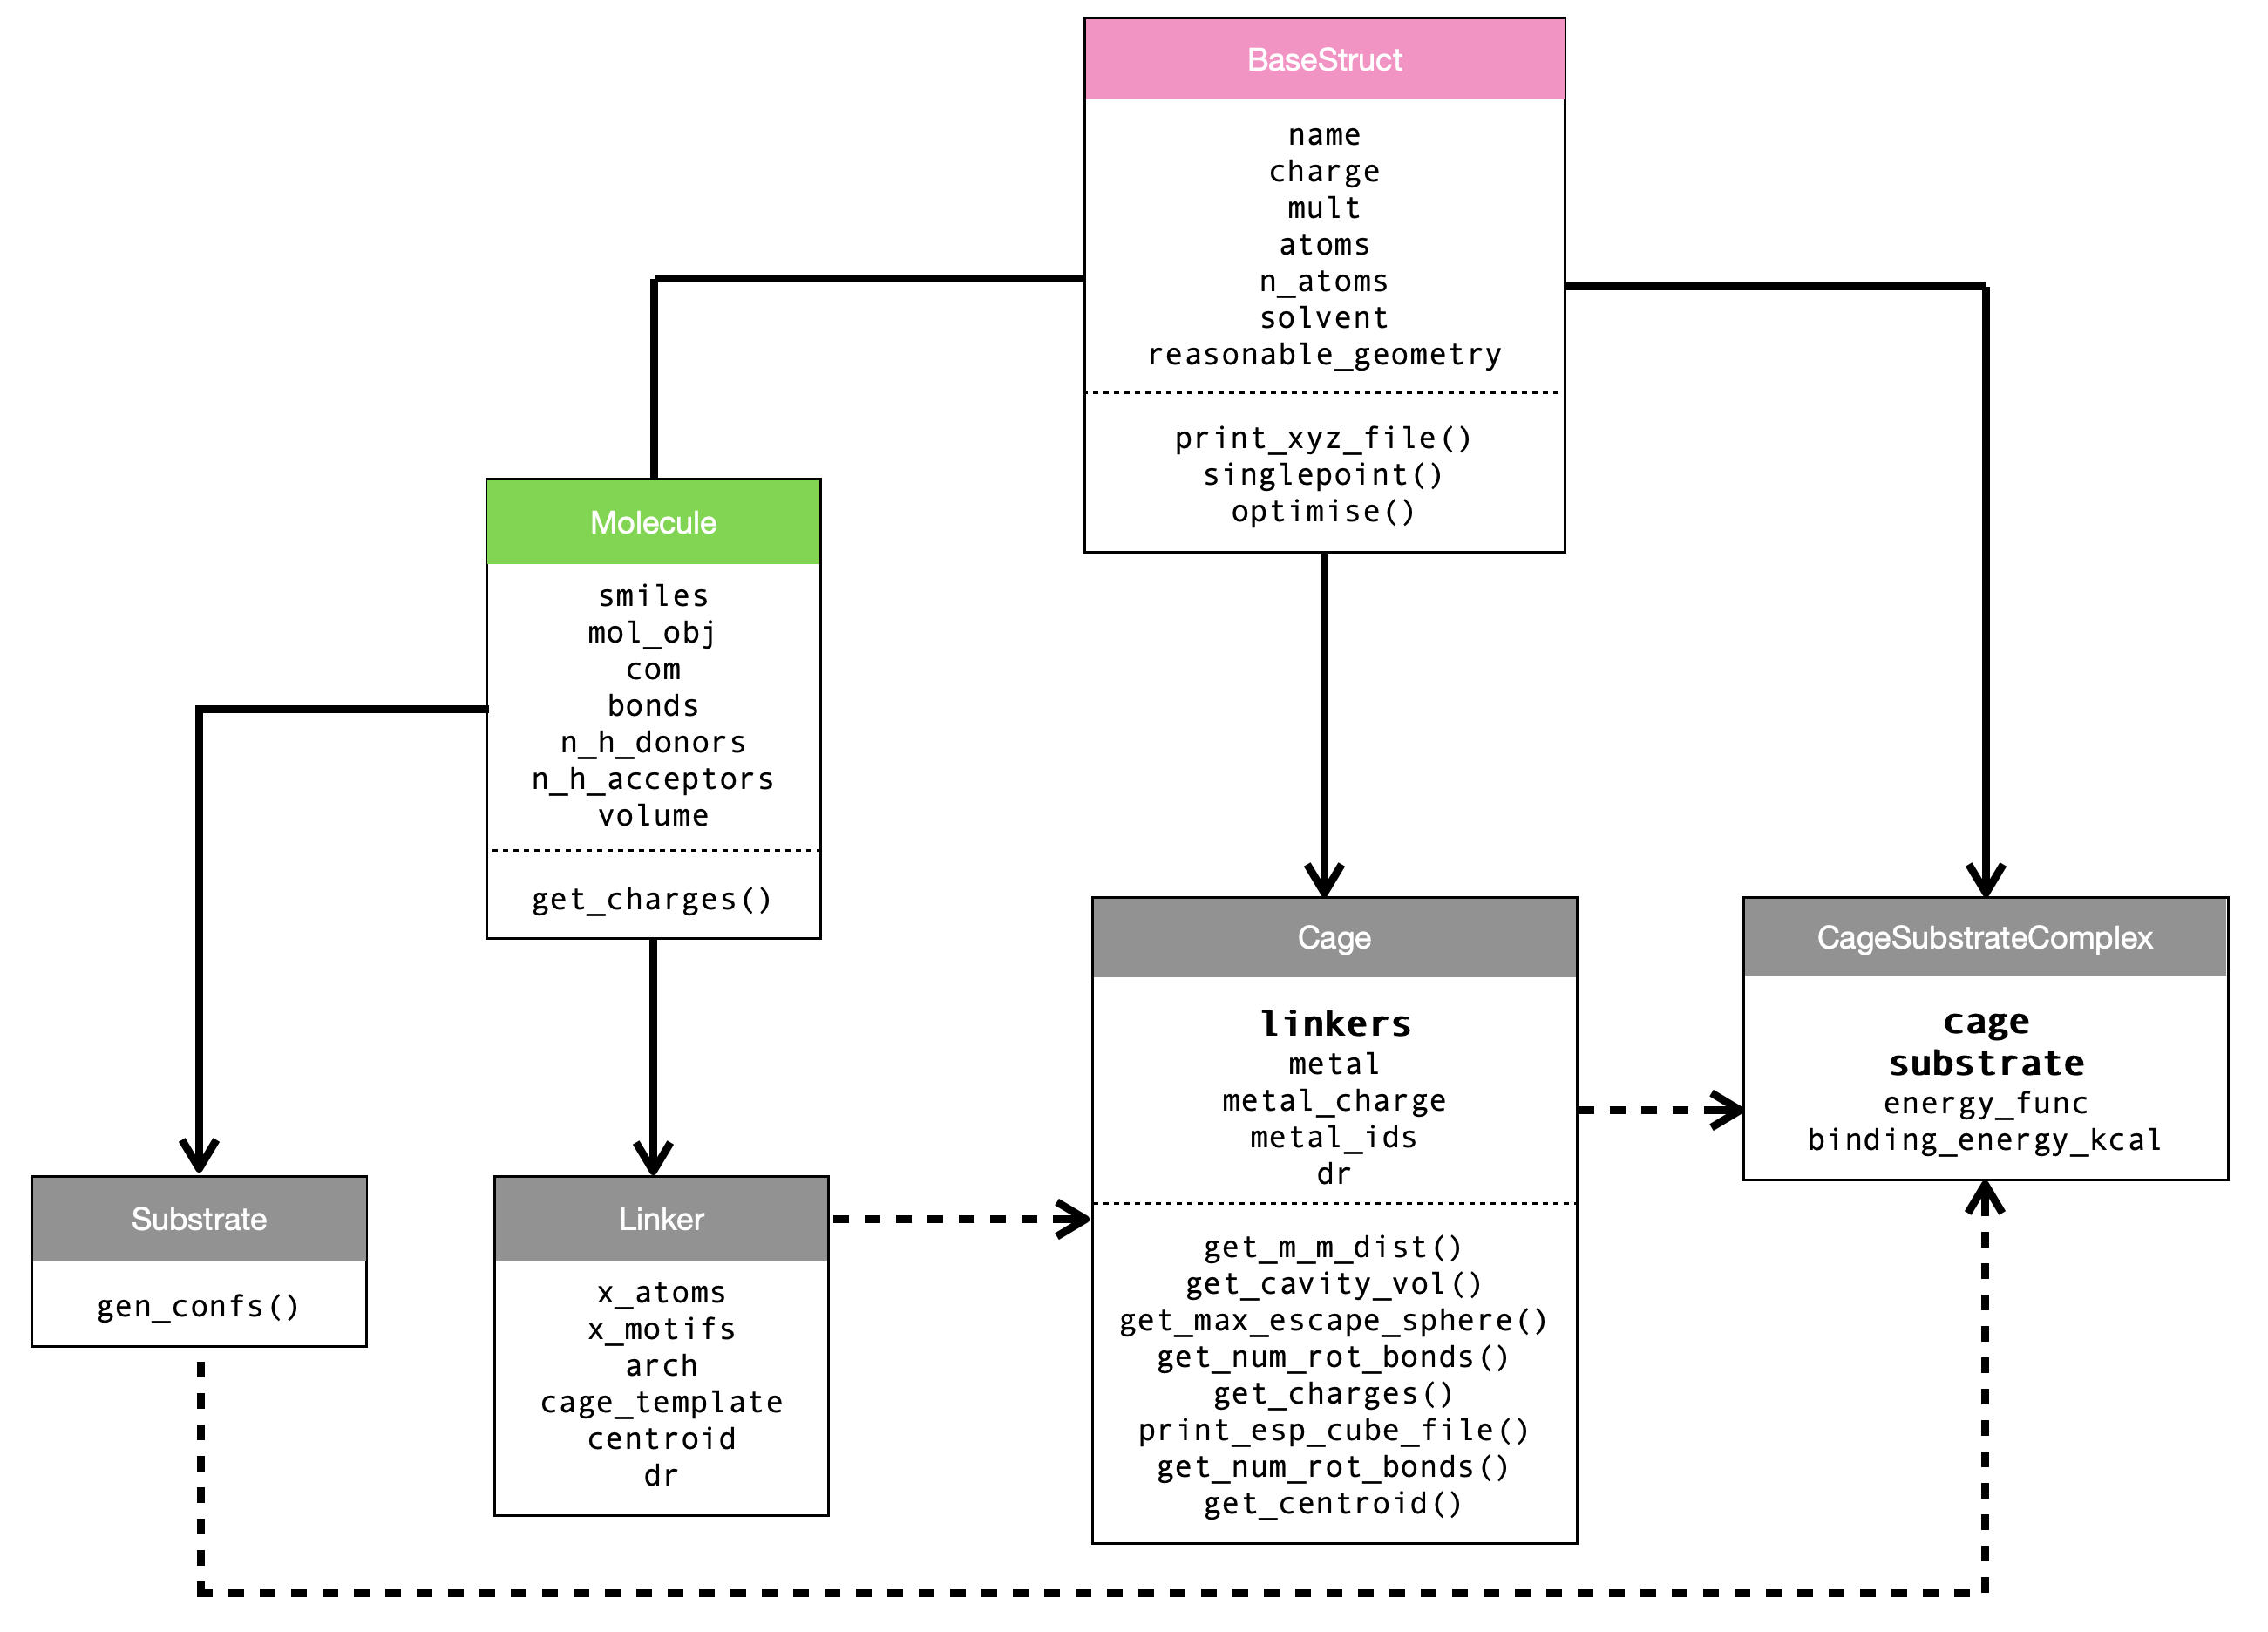
\includegraphics[width=\textwidth]{3/cgbind/figs/fig1}
	\vspace{0.2cm}
	\hrule
	\caption{Class structure of \emph{cgbind}. A solid line from A to B indicates that B inherits from A and a dashed line B is built from A.}
	\label{fig::cg_1}
\end{figure}

A homoleptic \class{Cage} (M$_x$L$_y$ with $x$ metals and $y$ linkers) is initialised from a single \class{Linker} object, while heteroleptic (e.g. M$_2$L$_2$L’$_2$) variants from a set of different Linkers. All \class{Molecule} objects and their subclasses are designed to be initialized from SMILES strings,\cite{Weininger1988} with their corresponding 3D structures generated using conformer generation algorithms implemented in RDKit.\cite{Landrum2019, Riniker2015}  While this affords rapid access to 3D structures, conformers are occasionally not adequately generated (see below). Molecules can also be initialized from a variety of molecular file formats (.xyz, .mol, .mol2) using the input\_output module. Upon \class{Cage} construction a number of analysis tools are available as class methods. The analysis of cage-substrate complexes (\class{CageSubstrateComplex} objects) is also possible. They are built from a \class{Cage} and one \class{Substrate}, where a substrate may contain more than one molecule, thus multiple guests are supported. Furthermore, a \class{Substrate} can either be a minimum or a transition state (/analogue), providing a route to predicting catalytic activity.
Binding affinities between a substrate (S) and cage (C) [\de$_\text{BA}$ = $E_\text{C-S} - (E_\text{C} + E_\text{S})]$ are calculated in the first instance using a simple and general forcefields developed here (see below). More accurate estimates can be obtained from electronic structure codes, by invoking singlepoint() and optimise() functions, which deliver energies (\class{Molecule.energy}) and optimized structures (\class{Molecule.atoms}). These functions are currently handled through a \class{Calculation} object in our Python API \emph{autodE},\cite{autodE} which facilitates the automated generation of reaction profiles. This enables \cgbind to utilize electronic structure packages with currently implemented wrappers (inc. GFN2-XTB,\cite{Bannwarth2019} MOPAC,\cite{Stewart2016} ORCA\cite{Neese2017} and NWChem\cite{Valiev2010}).

The structure of \cgbind benefits from modularity, allowing analysis functions to be implemented by simply adding methods to the \class{Cage} or \class{CageSubstrateComplex} objects. The fragment approach to generating a \class{CageSubstrateComplex} allows for all the properties of the cage, and constituent linkers to be contained within a single object. Linker, Cage and Substrate objects may therefore be reloaded from a saved (e.g. Pickled) \class{CageSubstrateComplex} object, allowing for data mining within a saved library. Independent calculations are parallelized up to the user-defined number of cores set in the \class{Config} object. The software is distributed under the MIT license and is provided with unit tests and comprehensive online documentation including examples.


\subsubsection{Metallocage Construction}
 Broadly, metallocage structures are generated from a SMILES or 3D representation of the linkers, which are templated onto known or user defined metallocage templates. The methodology employed is not template specific, such that extension to architectures other than those provided with the code (\MLf, M$_4$L$_6$, M$_6$L$_8$, M$_{12}$L$_{24}$) is straightforward. Figure \ref{fig::cg_2} provides an overview of the workflow behind \cgbind, which can be broken down into six key steps: 

\begin{enumerate}[label=\Roman*.$\quad$]
	\item        Generate $n$ linker (L) conformers from a SMILES string, a common way of representing molecules, which can be obtained from online databases (e.g. PubChem) or chemical software (e.g. ChemDraw\texttrademark).
	\item	The donor atoms bonded to the metal atoms (X-atoms) are located in L. 
	\item		Locate possible X-motifs, as all combinations of one or more X-atoms and their nearest neighbours in L.
	\item		Discard any X-motifs with a different number of atoms to the template X-motifs.
	\item	Minimize the fitting cost with respect to linker and template parameters. The fitting cost is defined as the sum squared distance (SSD) between the X-motif atoms in the template and L.
	\item		Fit linkers to the expanded/contracted template, controlled by a distance $\Delta r$, while keeping steric clashes below a threshold. 
\end{enumerate}


\begin{figure}[h!]
	\vspace{0.4cm}
	\centering
	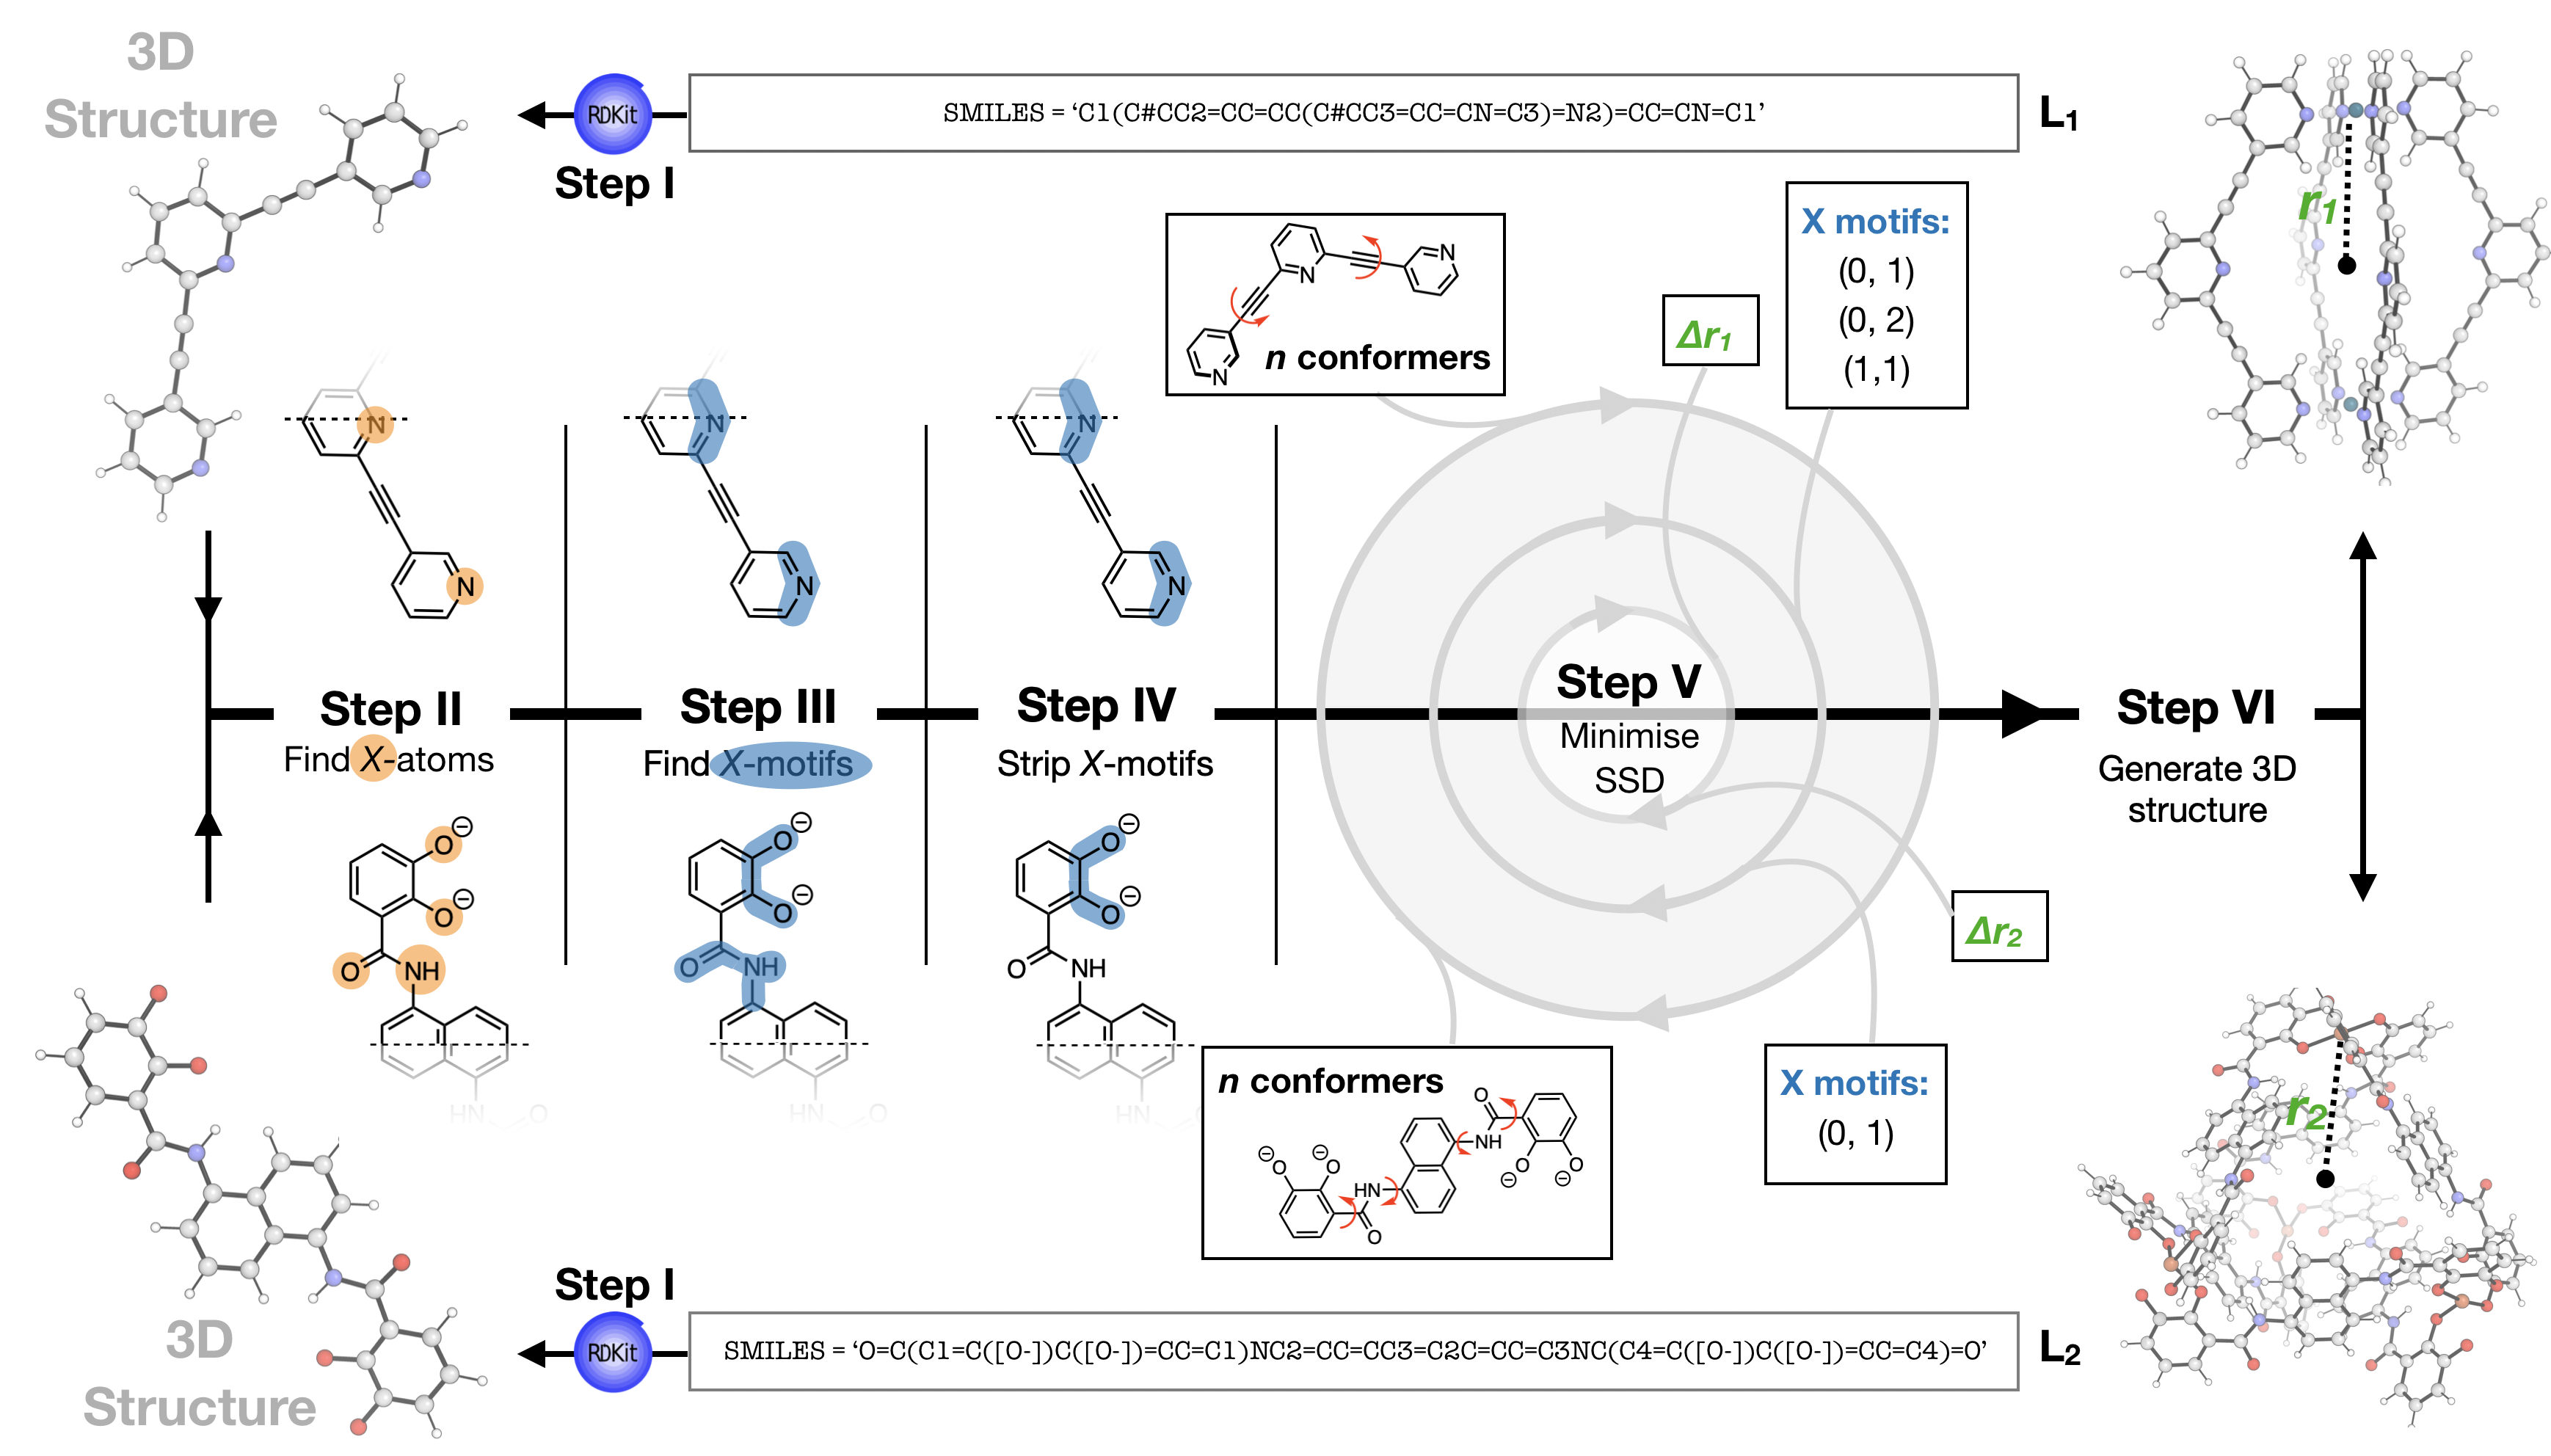
\includegraphics[width=\textwidth]{3/cgbind/figs/fig2}
	\vspace{0.2cm}
	\hrule
	\caption{Methodology used to construct metallocages in \cgbind. Centroid–metal distances are denoted as $r$ and shifts $\Delta r$. X-motifs are indexed from zero to the total number in the linker.}
	\label{fig::cg_2}
\end{figure}


These steps are discussed in detail below for two architectures, \MLf and M$_4$L$_6$, already saved in the template library. Note that, depending on the input provided by the user, not all steps must be executed. For example, if a Linker is initialized from a 3D geometry then the Step I can be skipped. Moreover, if the X-motifs are specified by the user then steps III and IV may be skipped, as well as minimization with respect to X-motif sets in Step V.

For a bis-pyridyl linker found experimentally to form a \MLf assembly (L1, top Figure \ref{fig::cg_2}),\cite{MartCentelles2018} the first step involves generation of 3D conformers using the Experimental-Torsion Distance Geometry with Knowledge (ETKDG) algorithm\cite{Riniker2015} implemented in RDKit\cite{Landrum2019} (Step I). For this linker, requesting 300 conformers and using a 0.3 \AA$\;$ root mean square displacement (RMSD) threshold to compare them, renders 50 conformers. This provided a good balance between speed and high probability of locating a suitable conformer. Subsequently, X-atoms are identified as the heteroatoms with at least one ‘lone pair’ capable of metal donation (here the nitrogen atoms, Step II). Combining X-atoms and their nearest neighbours affords three X-motifs containing CNC atoms (Step III). In the \MLf template, the X-motifs also contain three atoms (see §\ref{section::cg_2_2_2} for how these motifs are found); therefore, all X-motifs are kept (Step IV). Minimization of the fitting cost is then performed exhaustively with respect to all conformers and X-motif sets, and minimization with respect to expansion and contraction of the template is achieved using the Broyden–Fletcher–Goldfarb–Shanno (BFGS) optimisation algorithm implemented in SciPy\cite{SciPy} (Step V). The template is expanded/contracted by shifting the X-motifs closest to metal $i$ by the M$_i$–centroid vector a distance $\Delta r$. For L1, there are three X-motifs (top: 0, middle: 1 and bottom: 2, with 0 and 2 being equivalent), while there are only two X-motifs in the template linker; therefore, the three X-motifs in L1 can be fitted in three different ways, i.e. (0, 1), (0, 2) and (1, 2). X-motif atoms are fit to the template using an implementation of the Kabsch algorithm.\cite{Kabsch1976} Step V correctly identifies the linker with the most coplanar pyridyls as the optimum conformer, the two terminal CNC atom sets (0, 2) as the optimum selection of X-motifs and a small shift required in the template ($\Delta r_1 = 0.0037$ \AA). Upon sequentially fitting the optimum X-motifs in the linker to the adjusted template and adding two metal ions, a metallocage geometry is generated (Step VI). 

In an \MLs structure formed from identical catechol-derived linkers and Fe(II) (L${}_2$, Figure \ref{fig::cg_2}),\cite{Caulder1998} steps I/II proceed as for L${}_1$, while identification of X-motifs is slightly more complex. X-atoms are joined by their nearest neighbours to generate X-motifs for C-O-, C=O and CN(H)C and those separated by a one bond joined generating -OCCO- and O=CN(H)C motifs to give a total of 12 motifs in L2 (Step III). The template contains X-motifs with four atoms, thus only the -OCCO- X-motifs remain upon discarding those with greater and fewer than four atoms (Step IV). Steps V and VI proceed as for L${}_1$ but requires no enumeration over X-motif sets as both L${}_2$ and the template contain two X-motifs.
This strategy is amenable to heteroleptic cage generation; different linkers are generated within the same architecture and fitted in the order defined by the template. The template shift distance $\Delta r$ is taken as an average over all linkers, as to accommodate linkers with (slightly) differing lengths. For an experimentally accessible cis-M$_2$L$_2$L$_2$’ metallocage\cite{Zhu2018} the process is shown in Figure \ref{fig::cg_3}. We note that the trans isomer may be generated by simply reordering the linkers in the \class{Cage} initialization (i.e. \class{linkers=[linker1, linker2, linker1, linker2]} in Figure \ref{fig::cg_3}).


\begin{figure}[h!]
	\vspace{0.4cm}
	\centering
	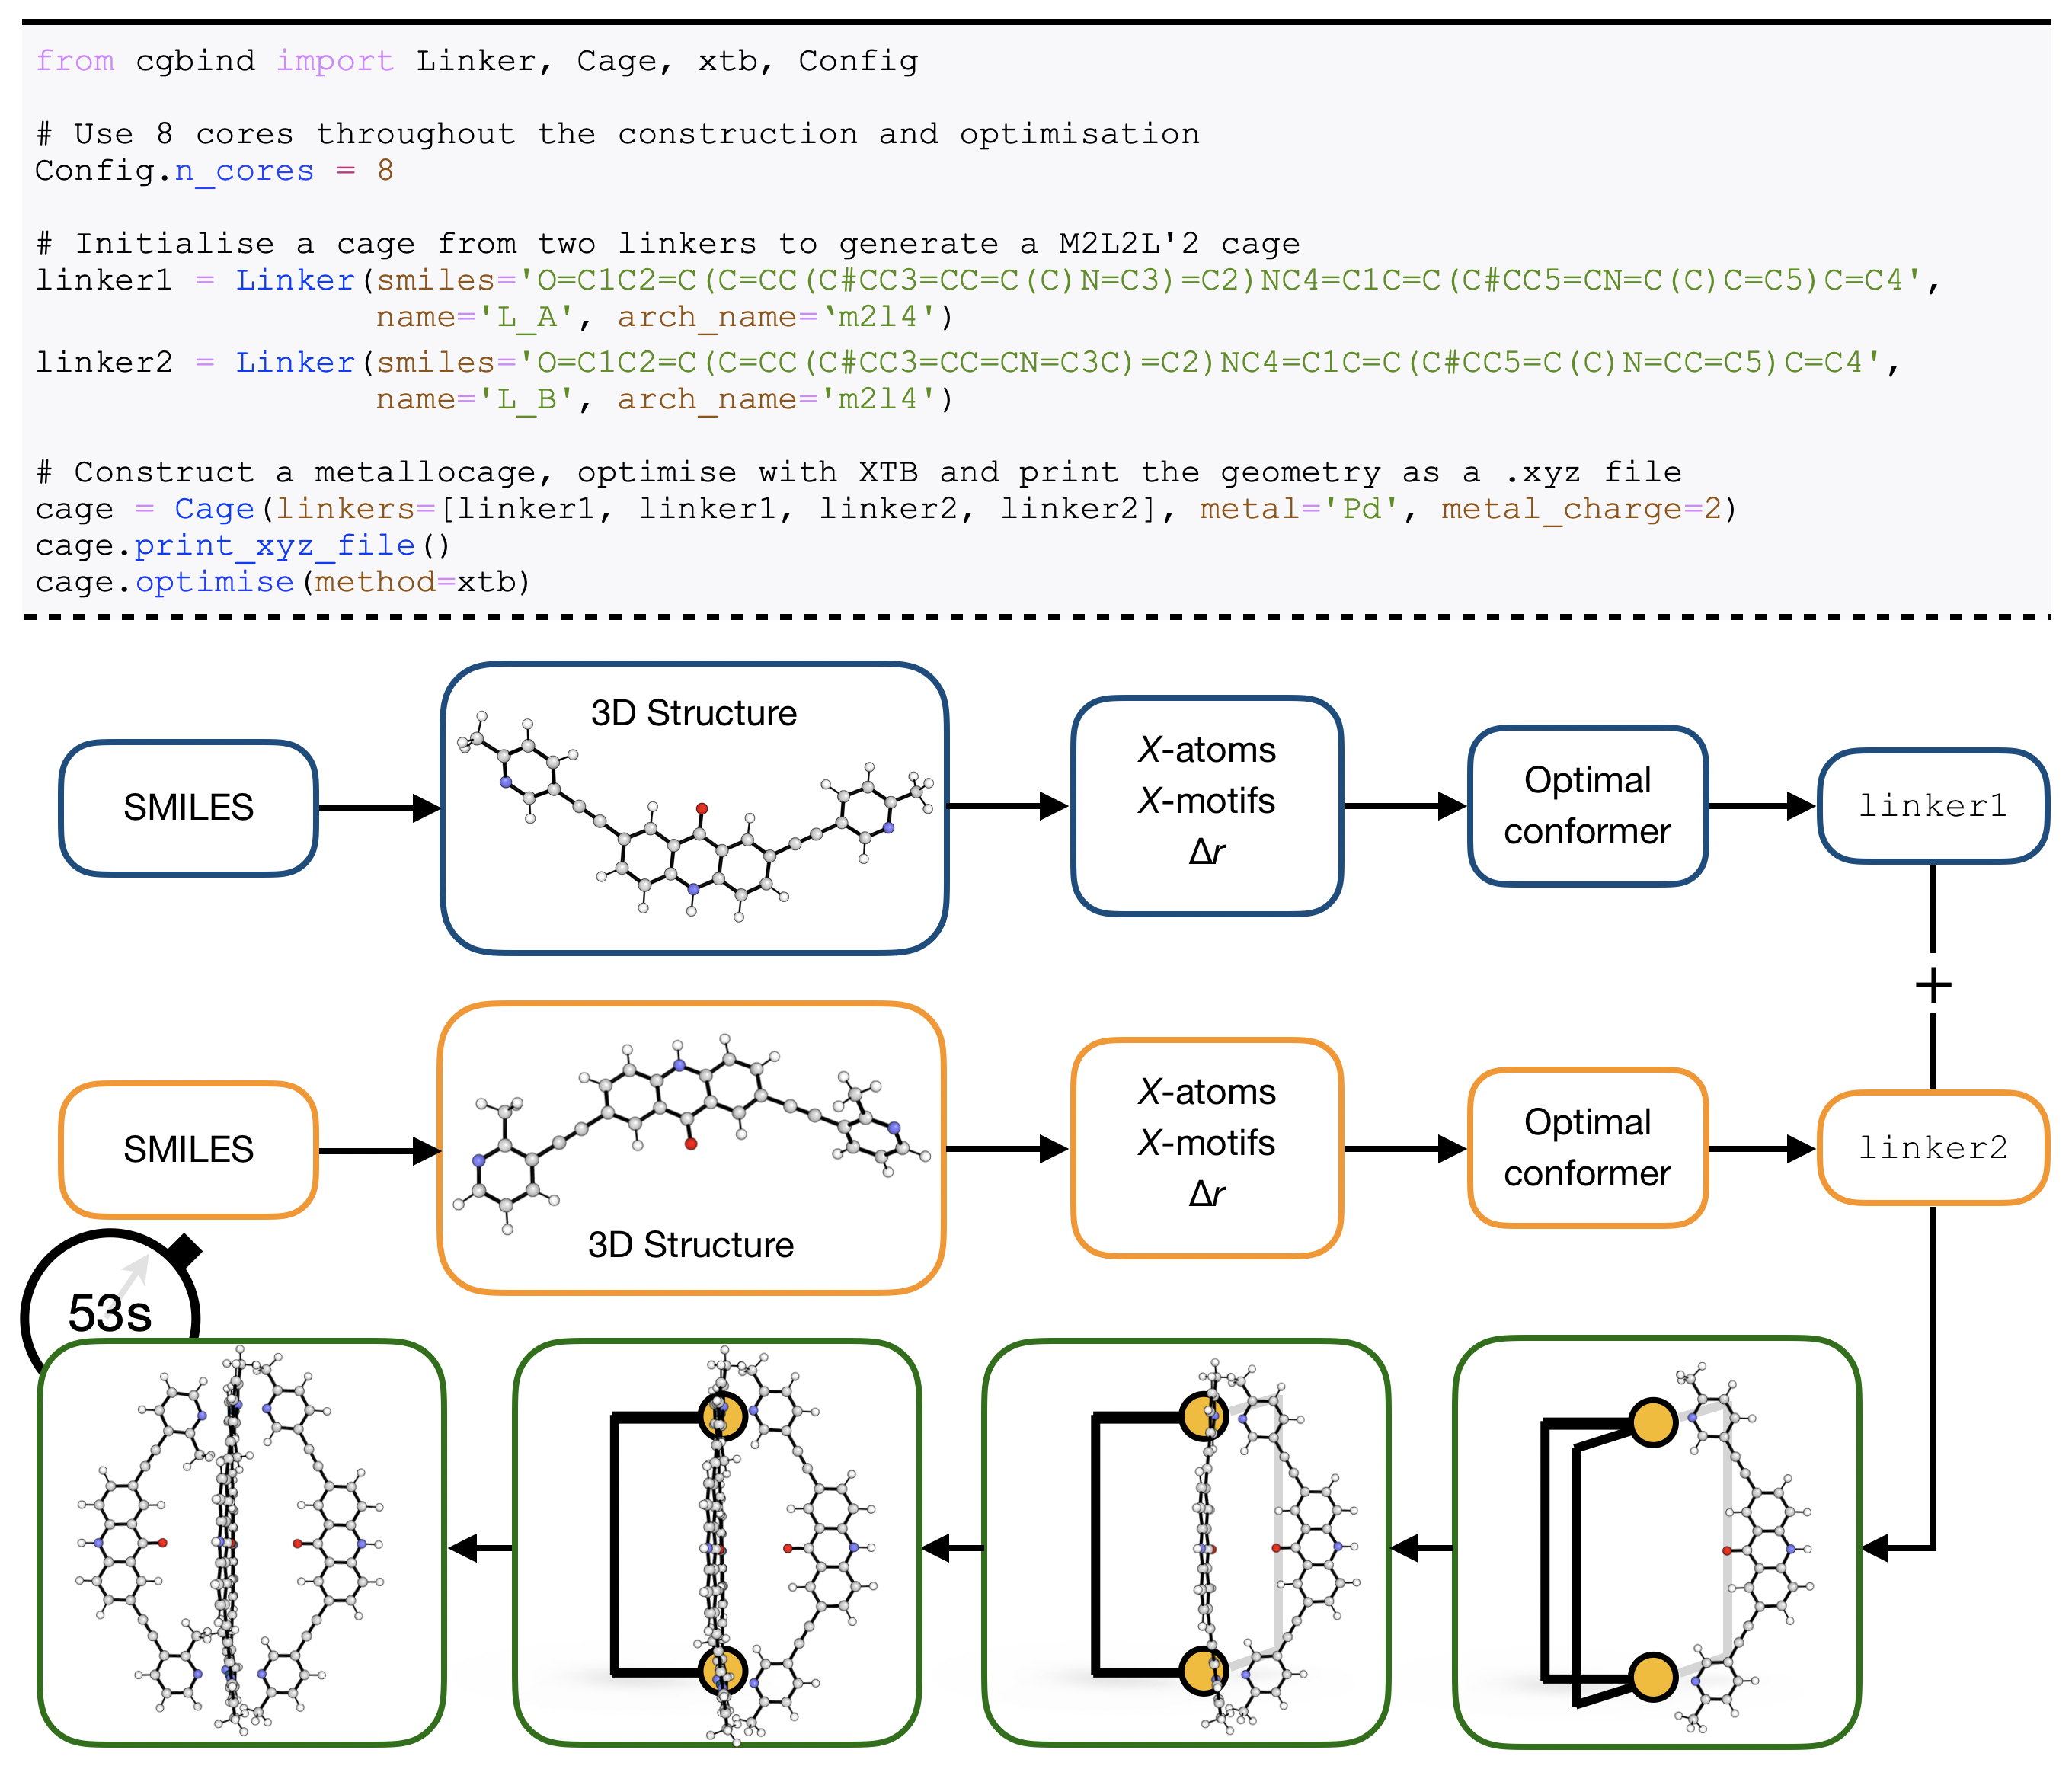
\includegraphics[width=\textwidth]{3/cgbind/figs/fig3}
	\vspace{0.2cm}
	\hrule
	\caption{Formation of a heteroleptic cage within \cgbind. Total execution time includes XTB optimization.}
	\label{fig::cg_3}
\end{figure}

For a linker with $n$ conformers, $j$ X-motifs in the template and $i$ metallocage X-motifs, the minimisation is conducted in a $\sim n \times {}^iC_j$ dimensional space. However, despite this large space, generally it is the conformer generation in RDKit, rather than minimization which dominates the execution time. Construction of cages with non-planar and or conformationally flexible linkers is facilitated by checking on the ordering of X-motifs and linker conformer as to achieve a threshold in the linker–partial cage repulsion during the build algorithm.


\subsubsection{Adding New Template Architectures} 
\label{section::cg_2_2_2}

Extensibility to new architectures is an essential feature of the code. The inclusion of new architectures by the user is achieved as follows: A 3D structure file (.mol2) is used for initialization of a Template. This structure can be downloaded from the CSD, or provided by the user (from non-deposited crystal structures or e.g. Spartan\cite{Young2001} generated constructs). 

\begin{enumerate}[label=\Roman*.$\quad$]
	\item Utilizing NetworkX a molecular graph of the system is generated. 
	
	\item A metallocage is identified as the molecular component with the largest number of metal atoms. All other molecules (ions, substrates) are stripped out; this step is required if the template is initialized from a crystal structure. 
	
	\item The donor (X-) atoms bonded to the metal atoms are located. 
	
	\item Linkers are identified by deleting metal atoms and determining its connected components using NetworkX.
	
	\item Within the linkers, and from the previously located X-atoms, X-motifs are located as the maximally connected set of X-atoms and their nearest neighbours.
	
	\item The shift vector for each X-motif is calculated to enable symmetric expansion of the template controlled by $\Delta r$ as above. 
\end{enumerate}

Overall, this workflow facilitates the addition of novel architectures into the code with minimal human intervention (i.e. a single command) and without structures needed to be hardcoded.


\subsubsection{Analysis Tools} 

Upon generation of a metallocage structure, \cgbind provides several geometry-based parameters that can be used to analyse and select metallocages for further binding and/or catalysis studies (Figure \ref{fig::cg_4}a). These include: (1) Number of rotatable bonds, which may be used as a proxy for cage flexibility (by default, the M-L bonds are not included).
(2) Total number of H-bond donors/acceptors, which can be used as a proxy for hydrophilicity. (3) Cage size metrics including  (i)	Average M–M distance.
(ii)	Maximum enclosed sphere: defined as the largest sphere centred on the cage centroid that does not contain any atomic (van der Waals) volume. The cage centroid is defined as the mean position of the metal atom centres.
(iii)	Maximum escape sphere: defined the largest sphere that may be removed from the cavity. This volume is determined by maximizing the sphere size at a distance $r$ from the cage centroid and taking the minimum sphere size along the path to the outside of the cage. 

The latter process can be performed with a basin-hopping algorithm from the SciPy library, which provides a more accurate estimate of the extrema but is computationally demanding.\cite{Wales1997} If the cage is symmetric, initializing with a random vector generally affords the largest escape sphere. However, for asymmetric cages, the use of a basin-hopping algorithm is necessary. This methodology is similar to that employed in pywindow\cite{Miklitz2018} and may be used as a proxy for window size, and consequently, substrate diffusion rates into/from the interior of the cage. 

Finally, (4) electrostatic potentials (ESP), which can be used to identify favourable guest-host complexes by maximising electrostatic interactions between them. By interfacing \cgbind with the open-source tight binding DFT code XTB,\cite{Bannwarth2019} ESPs can be obtained in seconds in the standard Gaussian cube format and visualized in PyMOL or other graphical software (\ref{fig::cg_4}b). This is achieved by performing a single point energy evaluation on the structure, retrieving the partial atomic charges (Mulliken population analysis) and constructing the ESP on a uniform grid as ESP($r$) = $\sum_i q_i/|r - r_i|$ in atomic units, where $i$ enumerates over atoms. Note that this approximation does not result in any loss in qualitative accuracy compared to the true integral over the electron density (Figure \ref{fig::si_cg_1}). 


\begin{figure}[h!]
	\vspace{0.4cm}
	\centering
	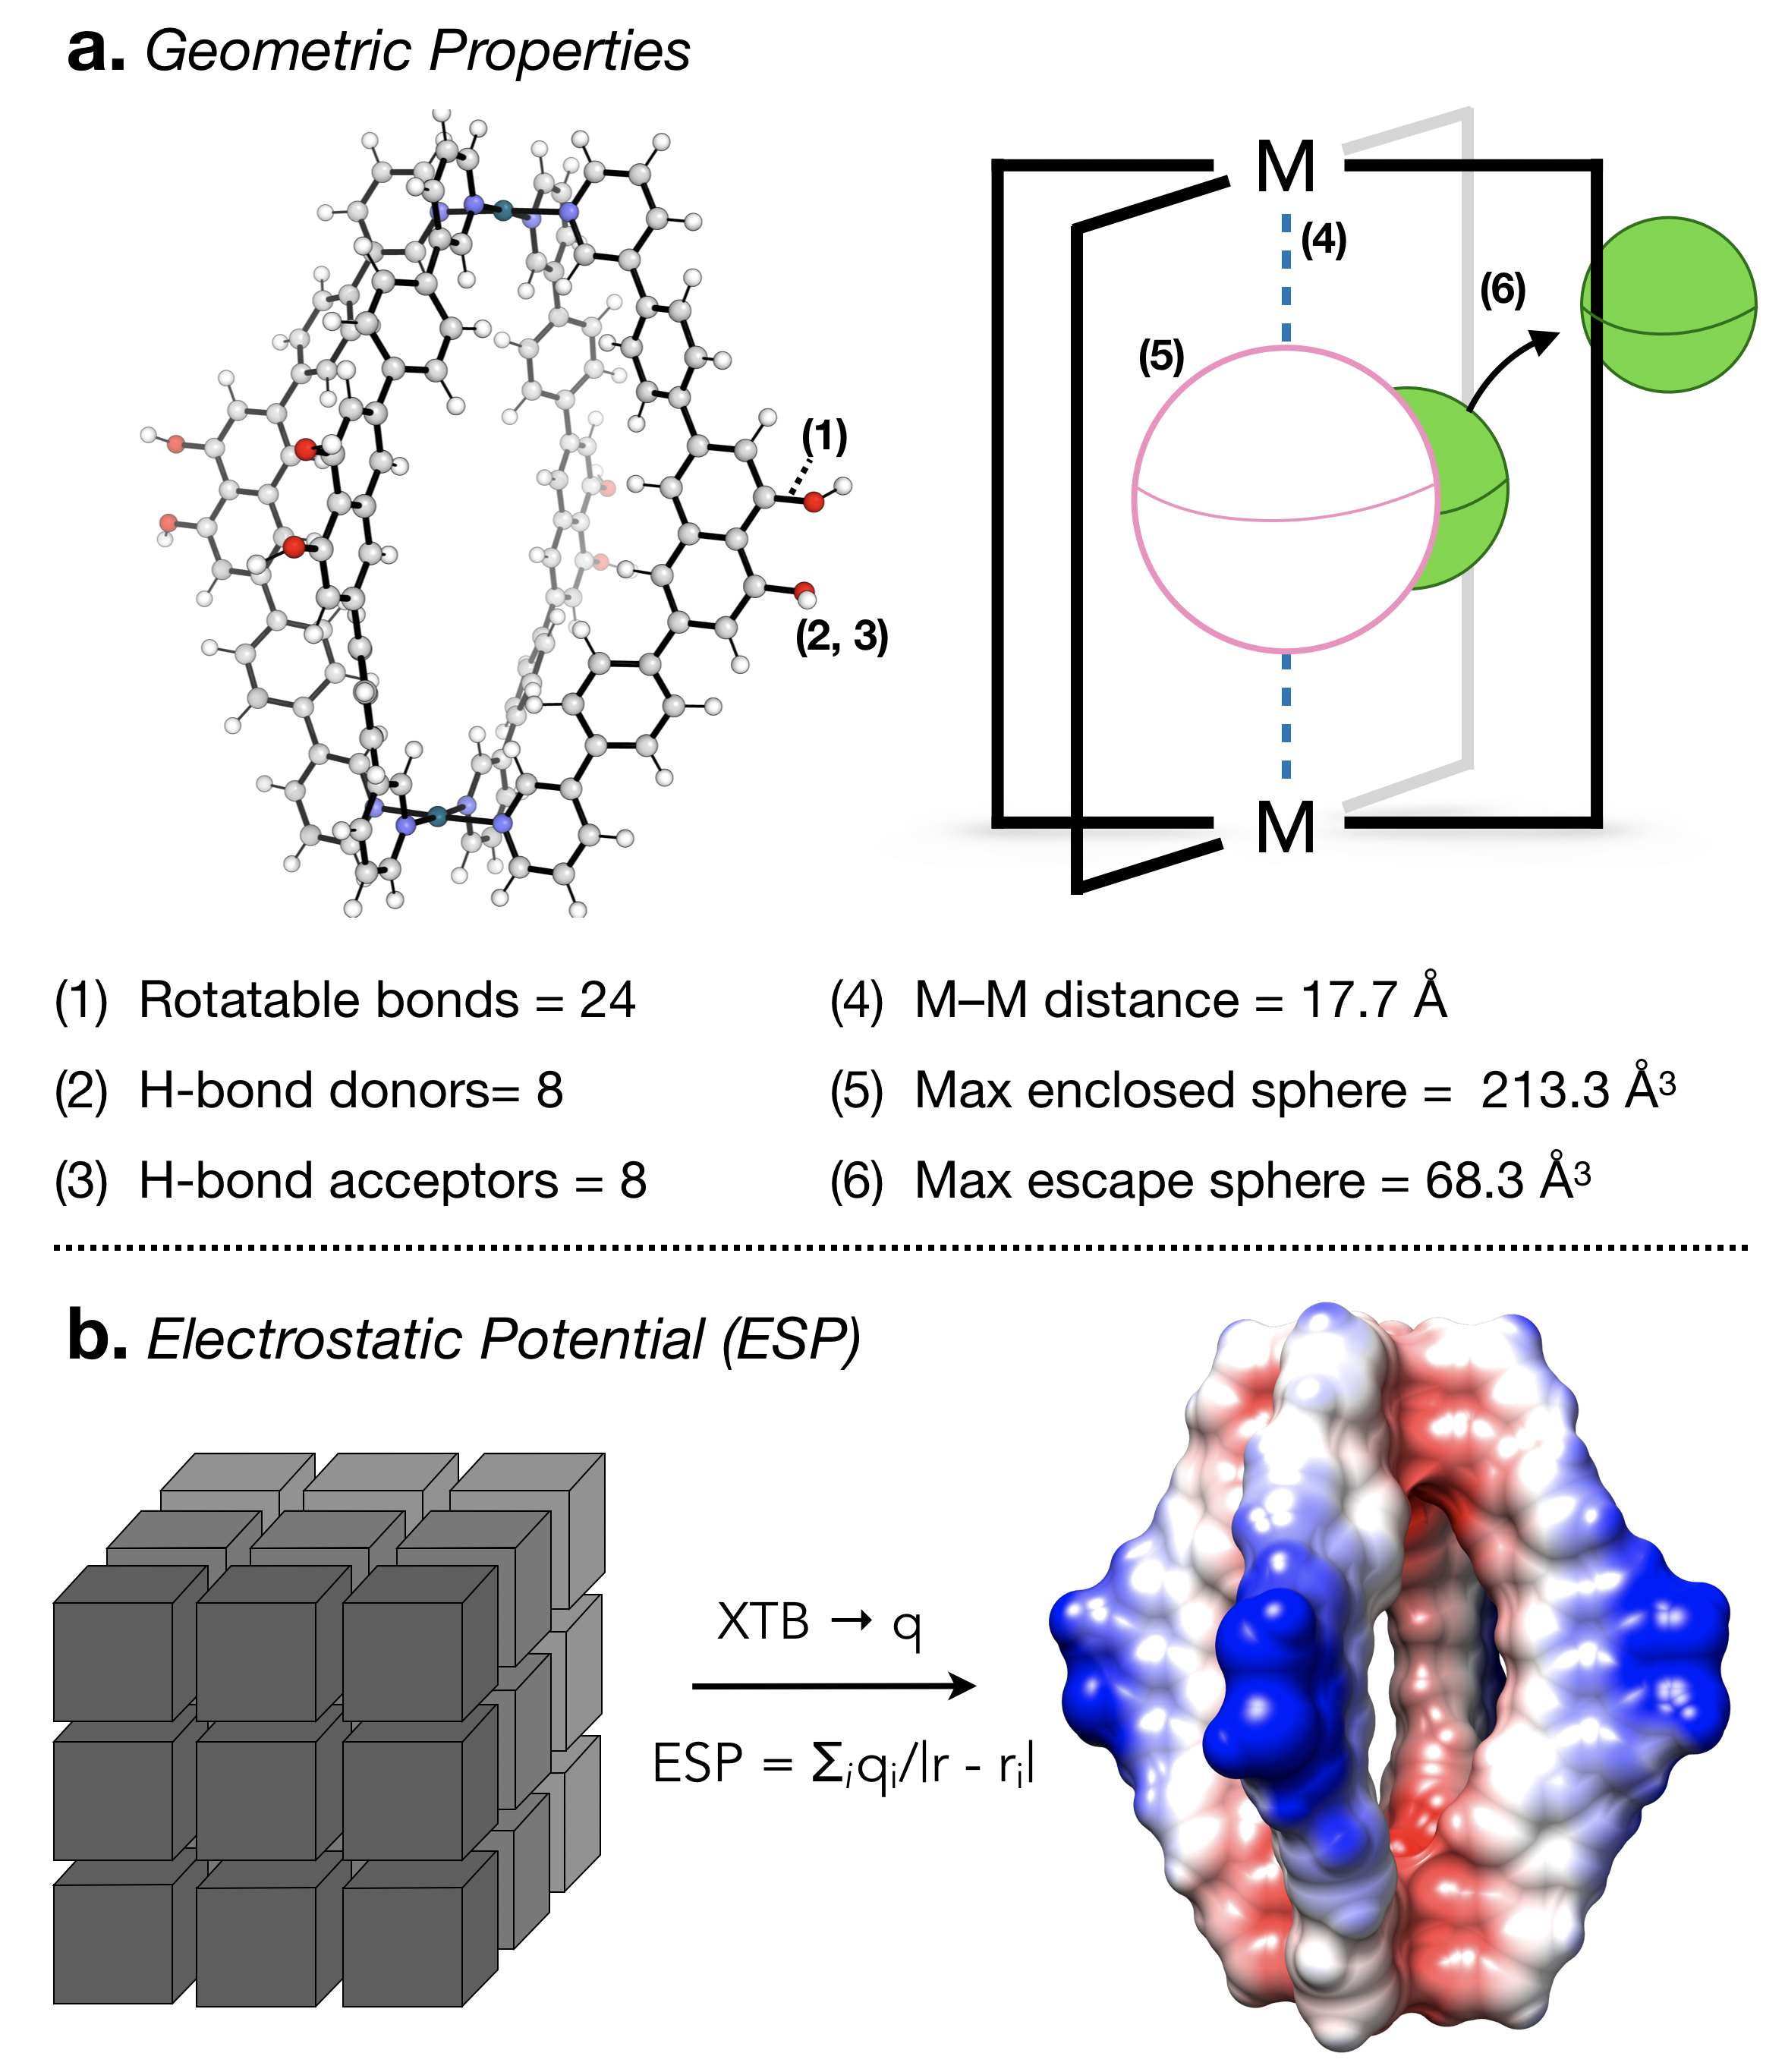
\includegraphics[width=12cm]{3/cgbind/figs/fig4}
	\vspace{0.2cm}
	\hrule
	\caption{Calculated metallocage properties for an archetype \MLf cage. (a) Geometrical properties: (1) rotatable bonds, (2) H-bond donors, (3) metal-metal distance, (4) maximum enclosed sphere and (5) maximum escape sphere. (b) Electrostatic potential (ESP) calculated from XTB partial atomic charges enumerated over a grid where blue/red corresponds to low/high values of the ESP.}
	\label{fig::cg_4}
\end{figure}
\clearpage


\subsubsection{Substrate Encapsulation and Binding Affinity Prediction}
 Once a metallocage is constructed, a substrate can be added to generate a cage-substrate complex. This is achieved by adding the substrate such that its centre of mass (COM) is located at the centroid of the cage in a similar way to ridged protein docking. The system is then energy minimized with respect to the substrate rotation and conformer, i.e. the global minimum on the rigid-body PES for each conformer is located (Figure \ref{fig::cg_5}). To obtain the global minimum a simple (random + BFGS) optimization algorithm is employed,\cite{SciPy} requiring $~\sim n\times m\times o$ energy evaluations, where $n$ is the number of conformers, $m$ the number of initial rotations and $o$ the number of BFGS optimization steps ($\sim20$). We have found that $m$ = 50 affords the global minimum with probability $\sim0.8$ for the systems tested (Figure \ref{fig::si_cg_2}). The number of conformers to screen is of course substrate dependent and is, as such, user specified.
Considering the large number of energy evaluations that would be required to evaluate binding of each conformer, electronic structure theory is not viable. To speed up this process we instead resort to empirical forcefields (FF). While a number of general FFs are available, their use is labour-intensive, requiring the tabulation of parameters and/or the use of specific molecular simulation packages. Furthermore, inherent approximations in their development limit their accuracy. To circumvent and simplify this problem, and assuming that substrate-cage interactions are dominated by sterics, we employed the following empirical energy function,

\begin{equation}
	E_\text{int}(r+k) = \sum_{i,j}^\text{pairs}  c \exp(a - |r_i - r_j|/b) +  k \times S_\text{atoms}	
\end{equation}

where the first half is a pairwise repulsive term, similar to the one found in a Buckingham potential, with $c$ = 1 and with units of energy. Using noble gas dimers as as a model for closed shell repulsion, we found that $a$ and $b$ are roughly linearly dependent on the sum of van der Waals radii (Figure \ref{fig::si_cg_3}). The second term is a constant attractive contribution ($k$) based on the number of substrate atoms ($S_\text{atoms}$). $k = 0.4$ \kcalx atom$^{-1}$ was derived as the optimum classifier for the set of binary binding data (see full SI). This approximation is considerable, as the attractive terms are dependent on the nature of non-covalent interactions (NCI) between the substrate and the cage (dispersion, H-bonding, etc.). Therefore, we only suggest using this FF to generate cage-substrate complexes where there the attractive term is expected to be small. We refer to this method as ‘repulsive’ $(r+k)$ and the binding energies arising from it as $E_\text{int}(r+k)$ (\code{energy\_method=`repulsion’}).

We have also considered a more physical FF, which utilises repulsive and electrostatic terms. The latter is calculated using either Gasteiger atomic partial charges from RDKit, which do not account for polarization of the atomic centres due to the surrounding environment (fe, \code{energy\_method=`electrostatic\_fast’}), or alternatively, charges derived from an XTB single point calculation which account for polarization effects (e, \code{energy\_method=`electrostatic’}). These methods more accurately account for NCI between the substrate and the cage. For example, within [Pd(II)$_2$L$_4$]$^{4+}$ metallocages, both schemes deliver the expected binding modes, which involves hydrogen bond interactions between the quinone oxygen and the C$_\alpha$-H groups at the top/bottom of the cage (Figure \ref{fig::cg_5}). 


\begin{figure}[h!]
	\vspace{0.4cm}
	\centering
	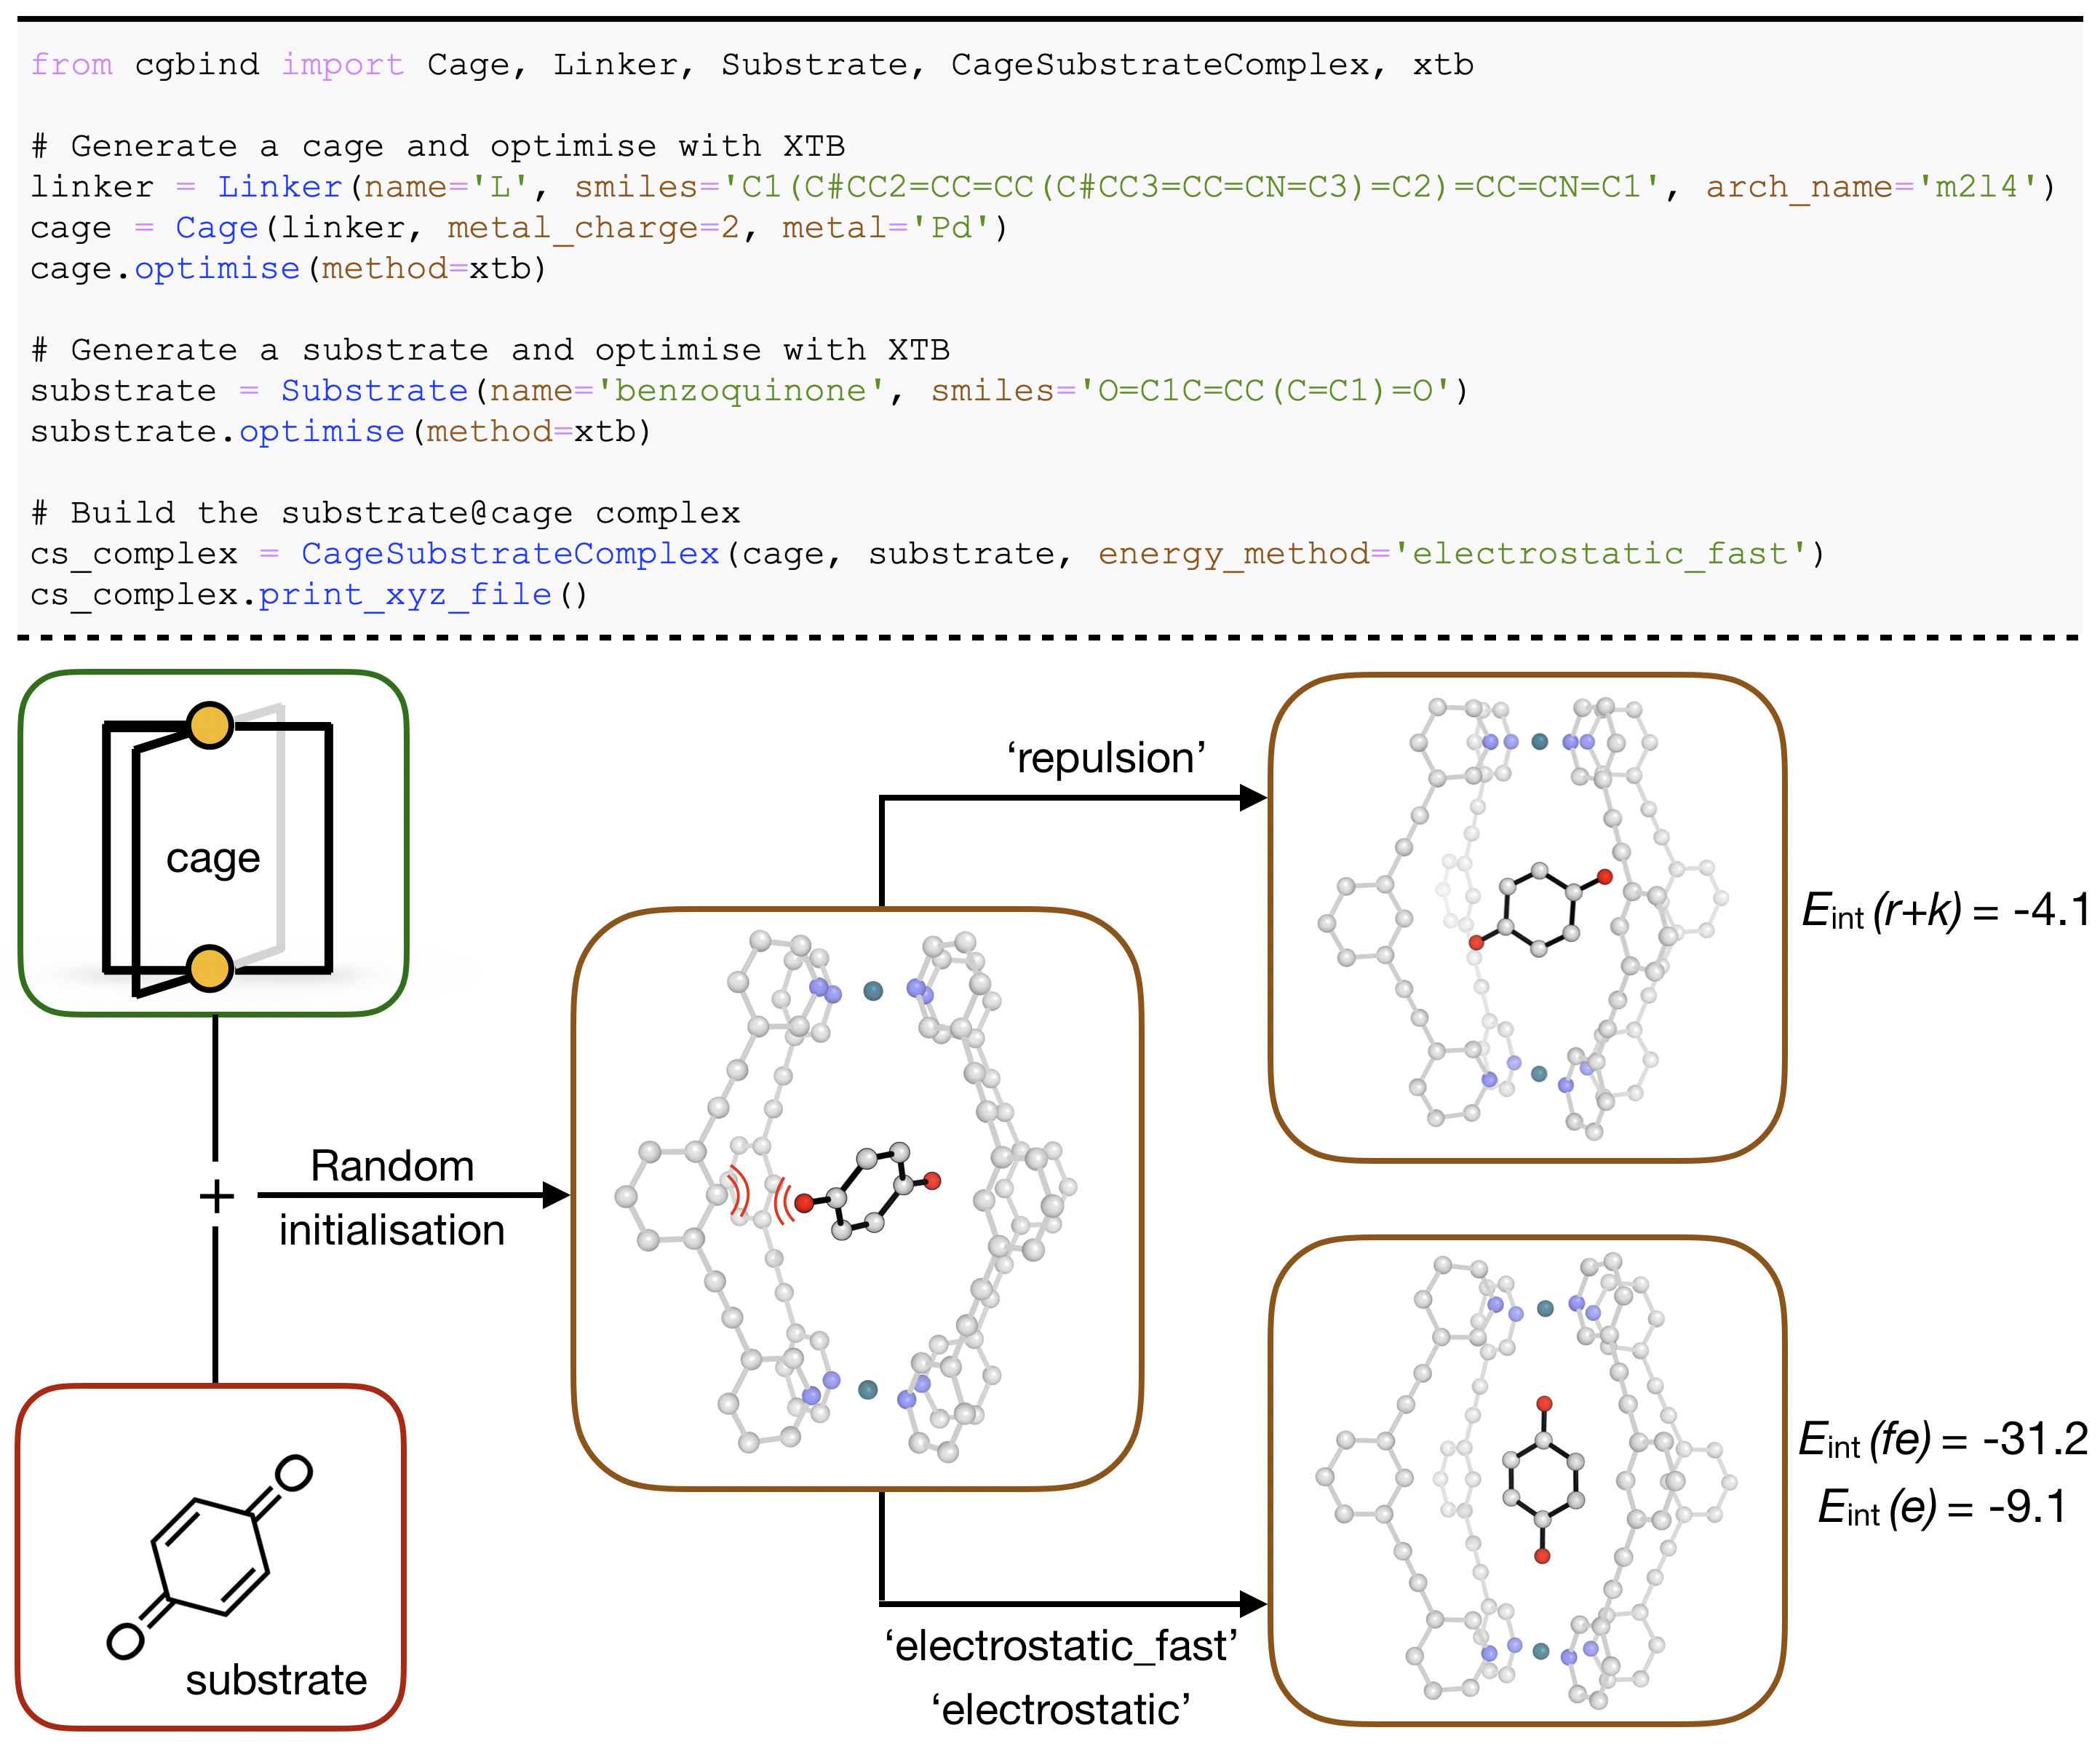
\includegraphics[width=\textwidth]{3/cgbind/figs/fig5}
	\vspace{0.2cm}
	\hrule
	\caption{Metallocage-substrate complex construction and interaction energy calculation for benzoquinone inside a [Pd(II)$_2$L$_4$]$^{4+}$ cage using the simple repulsive (r+k) and electrostatic forcefields (fe and e). Interaction energy predictions are quoted in \kcalx and do not include solvent, thermal or entropic contributions. Hydrogen atoms omitted for clarity.}
	\label{fig::cg_5}
\end{figure}

Quantifying the binding affinity of a given cage for a substrate is key in determining their applicability in real-world applications. In \cgbind, once the cage-substrate complex has been generated, an approximate gas-phase interaction energy ($E_\text{int}$) based on a simple FF above is available immediately, as it is minimised in the construction. This gives a rough estimate of the binding affinity and the likelihood of a cage to bind/not-bind a given substrates. A more accurate estimate can be obtained from electronic structure theory calculations, calculating either potential or Gibbs free energies in implicit solvent. The former we recently showed is sufficient to obtain quantitative agreement with experimental binding free energies for [Pd${}_2$L${}_4$]${}^{4+}$ metallocages.\cite{Young2019} Key sources of error in the calculation of free energies include inadequate quantification of entropy, sampling and errors in the methodology used.\cite{Zhou2009} Solvent effects can be accounted for implicitly using implicit solvent models implemented in electronic structure theory packages and are essential in modulating interaction energies, particularly in polar solvents. Moreover, \cgbind provides a starting point for free energy calculations required to treat explicitly solvated cavities. The free energy for cavity desolvation and subsequent substrate binding can then be obtained using all-atom molecular dynamics (MD) methods or by adding explicit solvent molecules to the cavity and using the ideal gas model (available in most electronic structure codes).


\subsubsection{Web app GUI}
 Alongside the Python interface we have also developed a web application as a GUI to the module. This approach allows a user to interact with key components of the code within a web browser, thereby reducing the activation barrier to its utilisation. Furthermore, by developing a web app the user does not need to download or install any packages/dependencies, which in many cases can be limited to specific platforms (Windows/Mac/Linux). The app is currently available at {\url{cgbind.chem.ox.ac.uk}} and provides the ability to: (a) generate and visualize a selection of metallocages, (b) perform analysis of metallocage size, (c) compute and visualize electrostatic potential maps, and (d) perform substrate binding calculations. SMILES strings of linkers can be pasted from chemical software packages, or generated in the \cgbind GUI using the 2D drawing tool Kekule.js.\cite{Jiang2016} Interactive molecular visualization of the generated structures is enabled using the open-source 3Dmol.js package, allowing useful actions such as rotating and zooming.\cite{Rego2015} The whole app is distributed in a microservice architecture [front-end (Flask), web-server (Gunicorn/nginx), message-broker (Redis), database (PostgreSQL) and task queue (Celery)] using Docker.


\subsubsection{Examples}
{\bfseries{Geometric Accuracy}}. To explore the ability of \cgbind to generate cages with varied topologies and linker functionalities we generated nine metallocages (a–i, Figure \ref{fig::cg_6}) and computed the root mean squared displacement (RMSD) of the heavy atoms to known crystal structures. With the exception of L${}_\text{h}$ (see below) all the metallocages were successfully generated from just the linker SMILES string all with RMSD $<$ 1.5 \AA. Geometry optimization of the structures at the tight-binding DFT level did, in some instances, improve RMSDs while for others (d, g, i) a larger deviation was obtained with the structure falling into a different local minimum. Similarly, optimization at the DFT level of theory (PBE-D3BJ/def2-SVP) provides no improvement in RMSD. This observation highlights the importance of accounting for the conformational flexibility of the linker and cage when constructing and analysing metallocages and their properties. We believe that this conformational variability provides an interesting avenue to explore substrate-dependent metallocage structure and function as well as a variety of allosteric effects. 

To generate a cage, the algorithm requires a conformer with donor atoms in the correct orientation. While conformational generation algorithms available in RDKit (ETKDG, ETDG) are generally adequate, for L$_\text{h}$ (Figure \ref{fig::cg_6}), we found that they do not afford a conformer with the torsion parameters required to generate a reasonable M${}_6$L${}_8$ metallocage, even with 104 conformers requested. Similarly, the open-source conformer generation implemented in OpenBabel (CONFAB),\cite{OBoyle2011} which performs well at generating structures close to that found in the crystal structure, does not afford the correct conformer from the RDKit initialized 3D structure.\cite{Ebejer2012} We note that the required conformer of L${}_\text{h}$ is 0.6 \kcalx more stable than the first RDKit generated analogue (Figure \ref{fig::si_cg_5}) and therefore should be generated in the conformer ensemble. This highlights the limitation of current conformer-generation algorithms. Therefore, Cage h was constructed from linker L${}_\text{h}$ which was built manually in the correct conformation and a Linker object initialized from an xyz file. Nevertheless, we consider our methodology to be robust in generating metallocages for varying architectures and multiple possible donor atoms. We also note that \cgbind provides reasonable structures in seconds rather than in hours (XTB) or weeks (DFT) for the largest metallocages shown in Figure \ref{fig::cg_6}.


\begin{figure}[h!]
	\vspace{0.4cm}
	\centering
	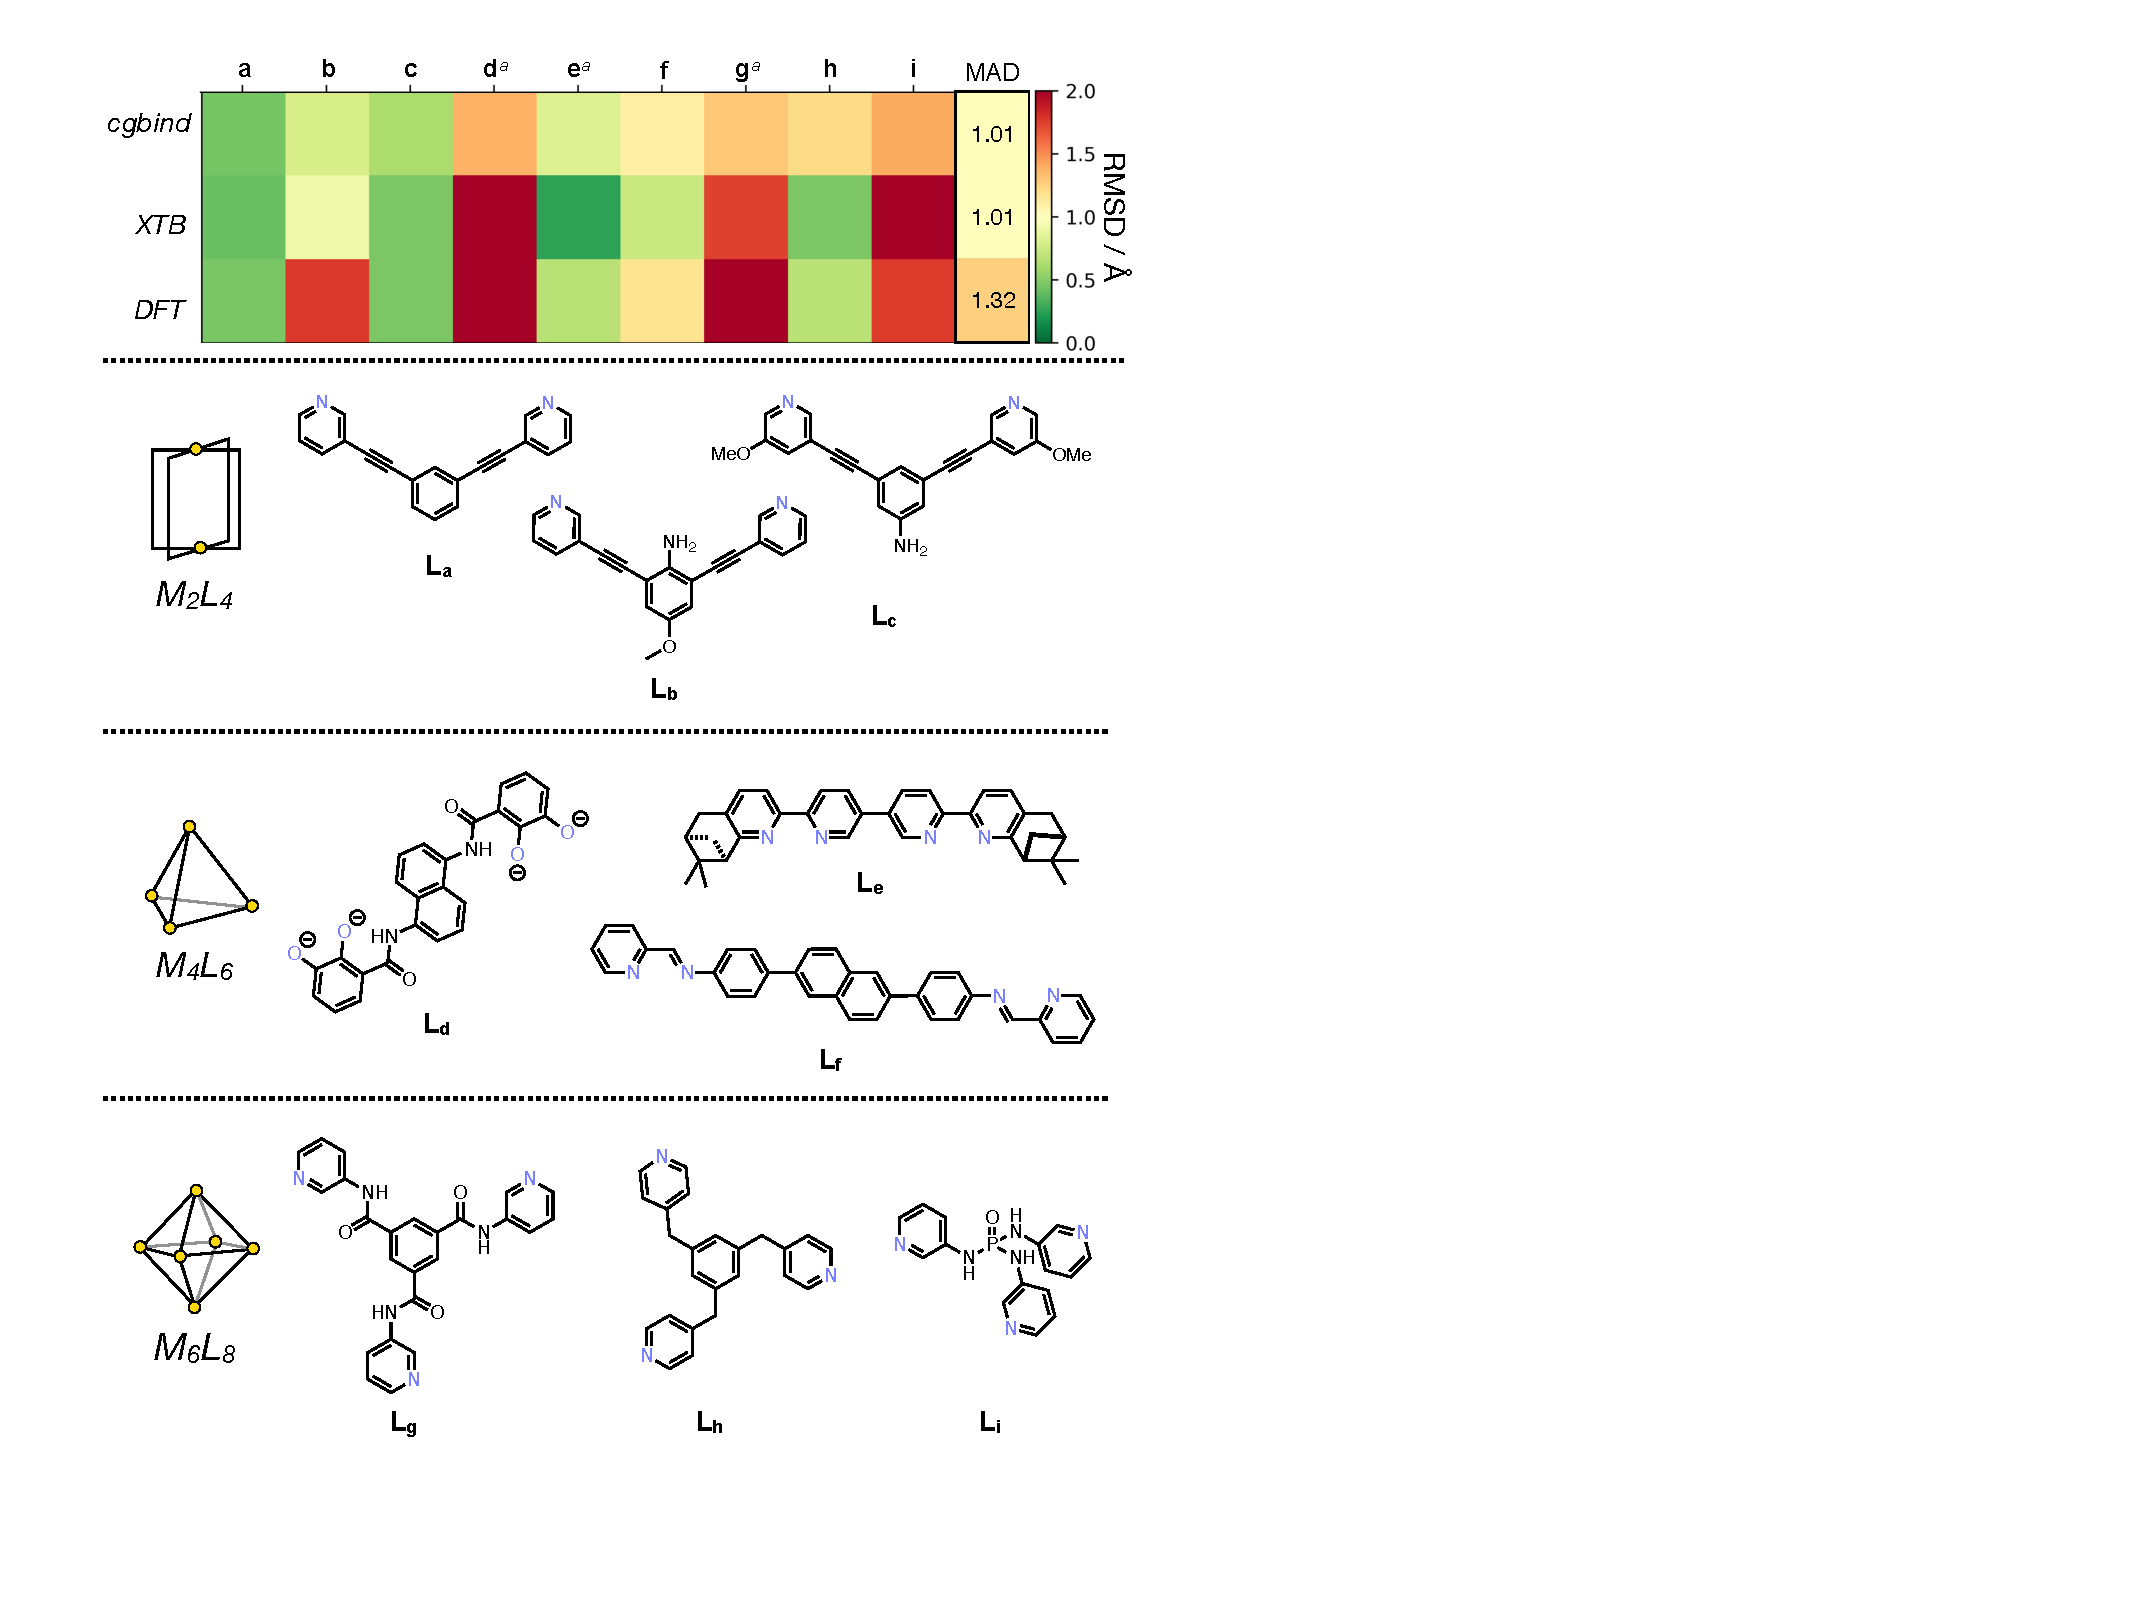
\includegraphics[width=13.5cm]{3/cgbind/figs/fig6/fig6}
	\vspace{0.2cm}
	\hrule
	\caption{Root mean squared deviation (RMSD, \AA) and their mean absolute deviations (MAD) of \cgbind-generated metallocage structures relative to available crystal structures in the CSD as a function of increasing computational expense, only heavy atoms were considered for the RMSD calculation. Counterions/solvent molecules in the crystal structures were removed for the analysis. Data in Table \ref{table::si_cg_1}. a. DFT geometries converged to a criteria only on forces (RMS(grad) $<$ 5 mHa $a_0^{-1}$).}
	\label{fig::cg_6}
\end{figure}

% Don't remove me to ensure correct formatting
\clearpage

{\bfseries{Binding Accuracy}}. For 102 host-guest complexes for which either quantitative or qualitative binding information exist in literature we explored the ability of cgbind to generate reasonable host-guest complexes and predict their binding ability. Those systems include \MLf and \MLs host architectures, and a range of polar and apolar substrates and solvents (dichloromethane, acetonitrile and water; see full SI). Specifically, the dataset includes: (1) 12 quinone‐type guests and two different Pd(II)$_2$L$_4$ cages (24 host-guest complexes in total). Their host–guest properties in dichloromethane and acetonitrile have been studied by Lusby et al.\cite{August2016} Depending on the nature of the quinone guest, binding constants of up to 108 M${}^{-1}$ have been observed for these systems. Many of them have also been found to be useful substrates in Diels-Alder reactions and cofactors in radical-cation cycloadditions.\cite{MartCentelles2018, Spicer2020} (2)	Six different guests, including polycyclic aromatic hydrocarbons and steroids, with a series of nine aromatic-panelled Fe(II)$_4$L$_6$ tetrahedral cages in acetonitrile studied by Nitschke et al. (54 hots-guest complexes in total).\cite{Ronson2017} In this cage series, the size and arrangement of the aromatic panels were suggested to dictate guest binding propensity. 
(3)	24 neutral and charged guests bound to Fe(II)$_4$L$_6$  tetrahedral cages studied by Nitschke et al.,\cite{Smulders2013} of which 21 were experimentally found to bind with binding constants ranging from 3 up to 104 M$^{-1}$. The host-guest properties of these systems in aqueous solution were found to strongly dependent on the hydrophobicity of the guest.

Cage substrate complexes were initialized using a single conformer in most cases, with the exception of cholesterol where 50 conformers were considered. In all cases reasonable host-guest complexes were obtained. To qualitatively explore binding affinity, and as a first approximation, we consider the experimental data and our prediction as binary classifiers, i.e. either the guest is observed to bind or not within the cage. The binding affinity is considered to be accurate if $E_\text{int} < 0$ for substrates experimentally reported binds. This approximation assumes that these experimental data can be directly compared and that only host-binding interactions determine binding, omitting the effect of solubility of the substrates and building blocks and the effect of entropy upon binding. 

Interestingly, the interaction energies calculated using our simple repulsive ($r+k$) and both fast and normal electrostatic forcefields (fe and e, respectively) are comparable to those achieved at the tight binding DFT level of theory (XTB) with implicit solvent, and considerably better than single point calculations at the semi-empirical PM7-COSMO level of theory, which provides a statistically different prediction and is considerably worse than our forcefields and XTB (Figure \ref{fig::cg_7}). Optimizations at the PM7 level were not performed as we have previously found that this leads to unphysical metallocage geometries.\cite{Young2019} Overall our accuracy is modest, $\sim$60 \%. This includes excellent ($>80$ \%) accuracy for \MLf cages with quinone guests, while for \MLs cages with aromatic guests the accuracy is limited to $\sim$40 \% (Figure \ref{fig::si_cg_8}). We hypothesised that the low accuracy of our FF and single point energy evaluations in the \MLs instance was due to the lack of cage relaxation not captured by our ridged body docking approach. To test this, XTB geometry optimisation were performed for the cage, substrate and cage-substrate complexes and the binding affinities evaluated again. In this case, all guests are predicted to bind, leaving the obtained accuracy static at $\sim40 $\% (Figure \ref{fig::si_cg_8}). For a representative example that does not bind experimentally we performed optimisations at the DFT (SMD(MeCN)-M06-2X/def2-TZVP//PBE-D3BJ/def2-SVP) level and found that the interaction energy was still negative ($E_\text{int} = -5$ \kcal) suggesting that XTB it is not the origin of the limited accuracy (Figure \ref{fig::si_cg_9}). Instead, thermal and entropic contributions, not accounted for here, are expected to shift the binding preference for this series. However, their consideration is known to be costly and subject to major errors. Moreover, the assumption that both host/guest are soluble and therefore equally available in solution should be considered. Nevertheless, our FFs provide accuracy on par with optimisation at the tight binding DFT level in a matter of seconds, with a confidence estimate that suggests true binding substrates are unlikely to be missed (Figure \ref{fig::cg_7}b). 



\begin{figure}[h!]
	\vspace{0.4cm}
	\centering
	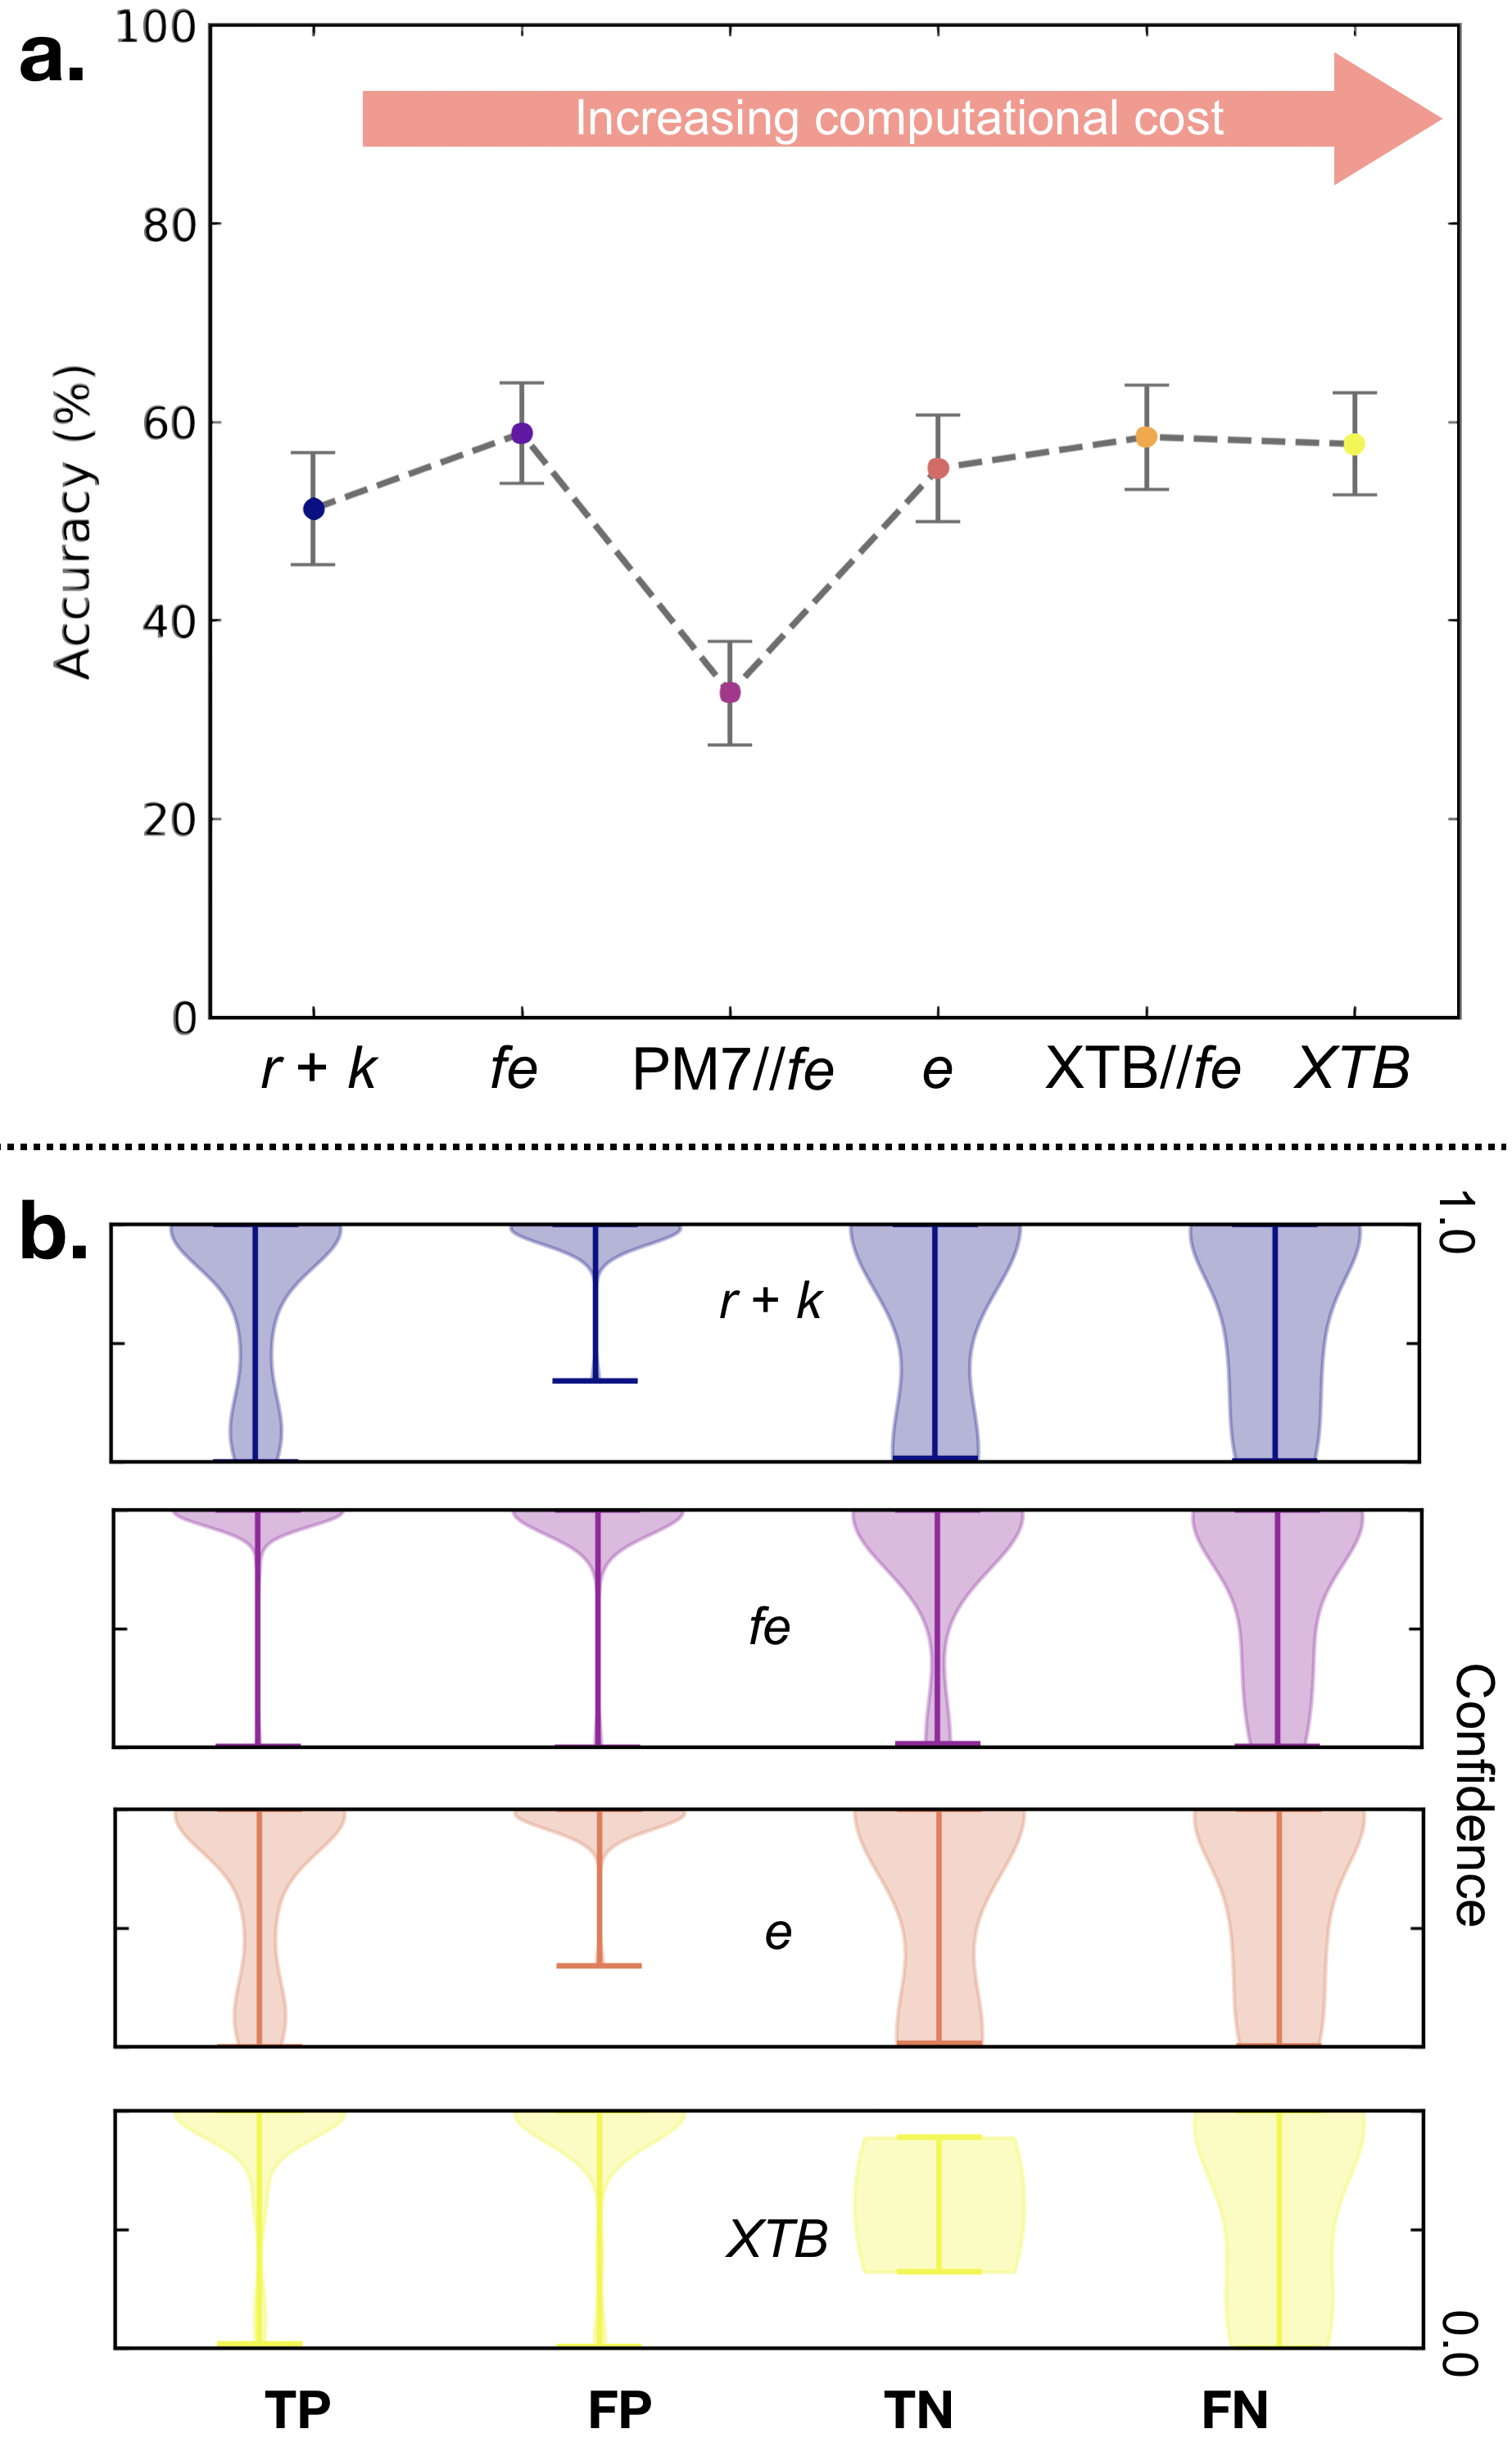
\includegraphics[width=9cm]{3/cgbind/figs/fig7}
	\vspace{0.2cm}
	\hrule
	\caption{(a) Percentage accuracy in predicting a substrate binds or not considering 102 host-guest complexes reported in literature. Experimental data tabulated in full SI. All binding calculations were performed within the \cgbind module interfaced through autodE to MOPAC and GFN-XTB. Error bars are plotted as a combined standard deviation, considering a small statistical error ($\sim$2 \kcal, Figure \ref{fig::si_cg_6}) with an assumed implicit normal error ($\sigma$ = 2 \kcal) and bootstrapping with replacement (10,000 resamples) on the dataset. (b) Confidence for true positives (TP), false positives (FP), true negatives (TN) and false negatives (FN) calculated as: $C = 1 - \exp(-(\Delta E/k)2)$, where $k$ = 5 \kcal.}
	\label{fig::cg_7}
\end{figure}

% Don't remove me to ensure correct formatting
\clearpage

{\bfseries{Combinatorial Metallocage Library}}. To demonstrate the ability of \cgbind to construct a library of cages from which subsequent property, screening and filtering calculations can be performed a library of Pd$_2$L$_4$ metallocages were generated (available for download as part of the Supporting Information). Employing linkers comprised of three ends (E), 12 links (Z) and 29 centres (C) building blocks, join linearly in a E-Z-C-Z’-E’ pattern and Pd(II) as the metal centre, a theoretical total of 13,104 homoleptic cages are possible (building blocks shown in Figure \ref{fig::si_cg_7}). From these, using linkers initialized with 200 conformers, 5,639 metallocages were constructed with ‘reasonable’ geometries (defined to be the minimum pairwise distance above 0.8 \AA, a higher proportion of cages would be constructed in a reasonable geometry were the linkers initialized with more conformers). Considering binding of benzoquinone as a guest, cages with cavity radii smaller than the centroid–O distance were removed to afford 1,353. This dataset was further reduced by eliminating those cages that were found to be too large to allow the formation of attractive NCIs between the substrate and the cage (cavity volume $>2\times$ substrate), leading to 914 cages. Employing the algorithm \code{electrostactic\_fast} to determine the optimal binding mode, 489 cages were removed based on $E_\text{int} > -15$ \kcal. Cages with formation energy [$\Delta E_f = E_\text{C} - (2E_\text{Pd} + 4E_\text{L})$ above 50 \kcalx of an optimised reference Pd$_2$L$_4$ cage reported in ref. \cite{August2016} calculated using XTB single point calculations were removed affording 275 cages. The most strongly binding hosts ($\Delta E_\text{int} < -12$ \kcal) were then taken forward. Finally, the three most synthetically accessible cages were selected, assuming the most accessible linker molecules lead to the most accessible metallocages, this was determined using the method from ref. \cite{Ertl2009} (Figure \ref{fig::cg_8}). From these core structures monovalent atom functionalisation e.g. H $\rightarrow$ Me, Et, Ph, CF$_3$ etc. may be performed using our Python module for molecular functionalisation ({\url{github.com/duartegroup/molfunc}}) to afford a vast library of heteroleptic cages.


\begin{figure}[h!]
	\vspace{0.4cm}
	\centering
	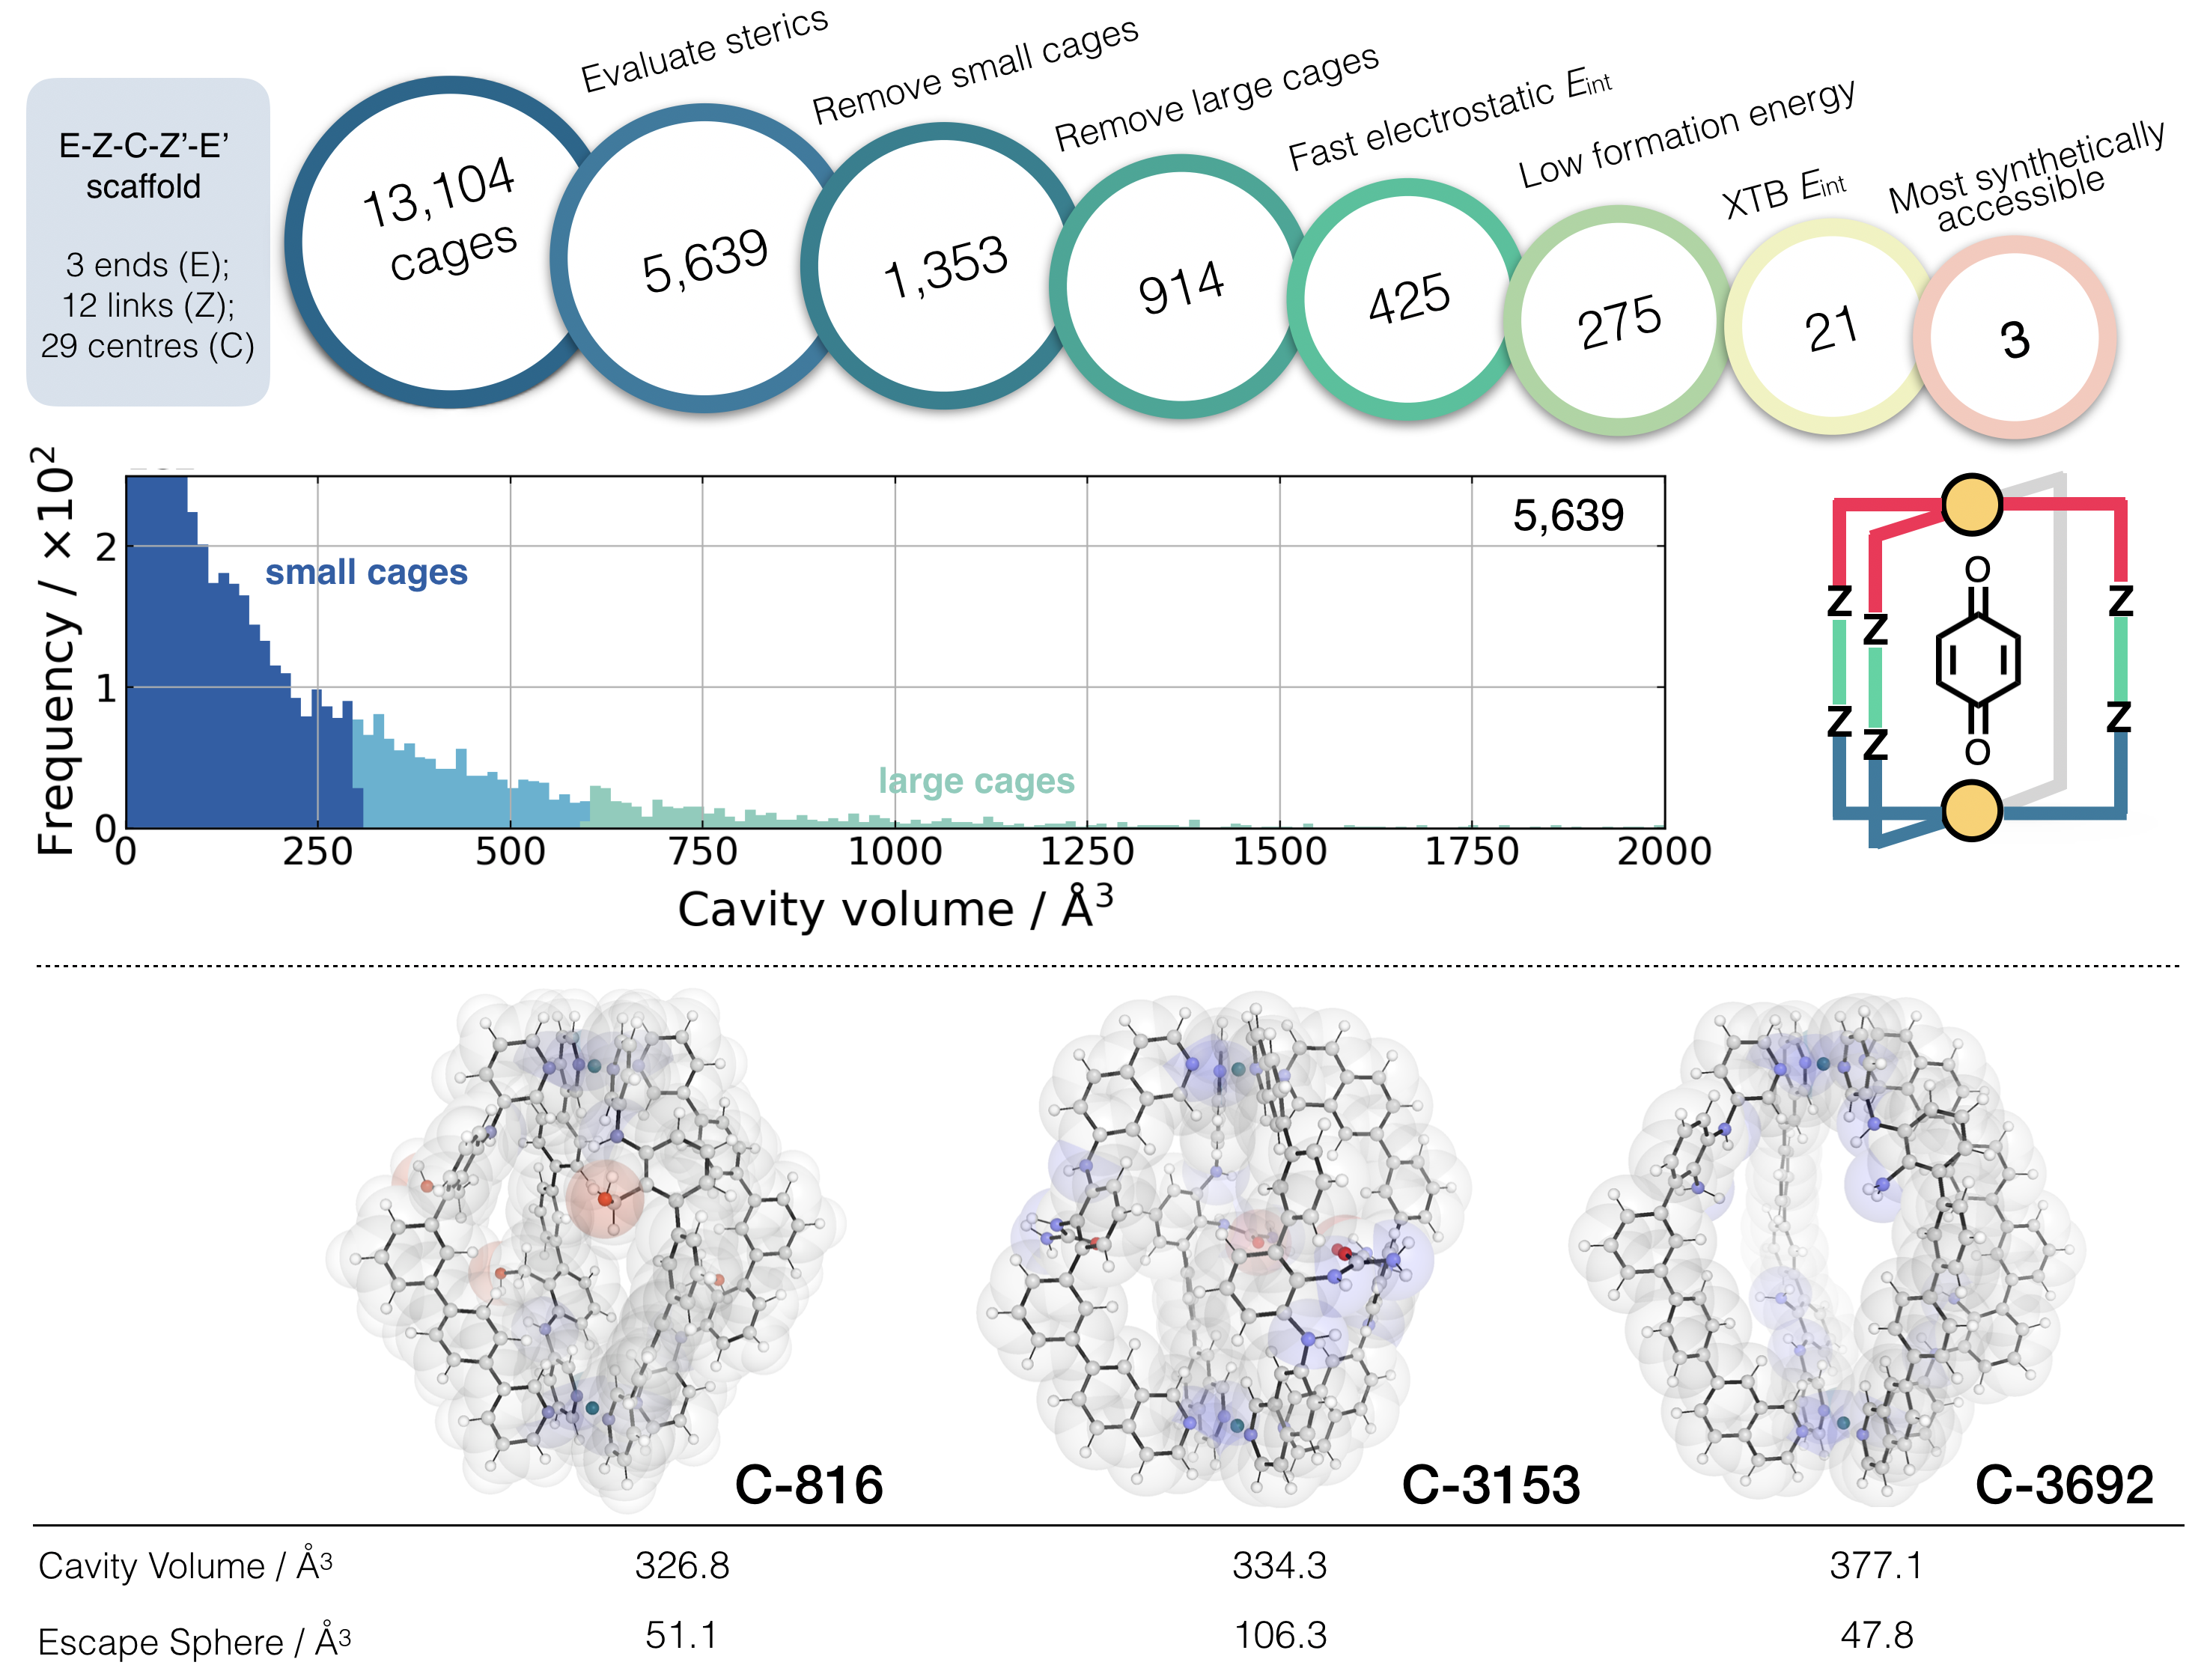
\includegraphics[width=\textwidth]{3/cgbind/figs/fig8}
	\vspace{0.2cm}
	\hrule
	\caption{Filtering process used to find the three optimal hosts for benzoquinone based on simple geometric criteria, tight-binding DFT calculations and synthetic accessibility of the constituent linker molecules. Building blocks shown in Figure S7.}
	\label{fig::cg_8}
\end{figure}

% Don't remove me to ensure correct formatting
\clearpage

\subsection{Conclusion}

Here we have described a modular and extensible Python module \cgbind for the automated construction and analysis of metallocage structure with arbitrary architecture (M$_x$L$_y$). Metallocages are constructed using a templating strategy and host-guest complexes generated by minimizing the energy of a simple forcefield developed here. Methods are available to analyse the resulting structures both qualitatively (electrostatic potential) and quantitatively (e.g. cavity size, window size) to analyse the resulting structures. We anticipate that \cgbind and its web-app ({\url{cgbind.chem.ox.ac.uk}}) will facilitate the rational design of functional metallocage with applications in binding and catalysis. Further work towards the reverse design of metallocages is ongoing, where rather than modifying linkers to subsequently build metallocages and search for tight complexation, the cage is built around the substrate to maximize binding.

\subsection{Computational Methods}

Root mean squared deviations (RMSD) were calculated using the Kabsch algorithm implemented in the \emph{rmsd} Python module,\cite{Kromann2019} reordering atoms and not considering hydrogens, all other parameters were set to their defaults. Metallocages had to be approximately aligned manually by fitting metal atoms prior to RMSD calculation, i.e. the reordering of atoms was not completely effective. All \cgbind computations were performed with v. 1.0.0 beta. Tight binding (TB-)DFT calculations were performed using GFN2-XTB v. 6.2,\cite{Bannwarth2019} PM7 using MOPAC2016,\cite{Stewart2016} and resolution of identity DFT using ORCA v. 4.2.\cite{Neese2017} Unless otherwise stated the latter using the PBE functional,\cite{Perdew1996} in combination with the D3BJ dispersion correction,\cite{Grimme2010, Grimme2011} def2-SVP basis set\cite{Weigend2005} (which employs effective core potentials for all metals used here)\cite{Andrae1990} and the default auxiliary basis sets.\cite{Weigend2006}


\clearpage
\section{Selected Supporting Information II}
\emph{Full Supporting Information including raw data can be found at:}\\ {\url{https://pubs.acs.org/doi/10.1021/acs.jcim.0c00519}}
\\\\


\begin{figure}[h!]
	\vspace{0.4cm}
	\centering
	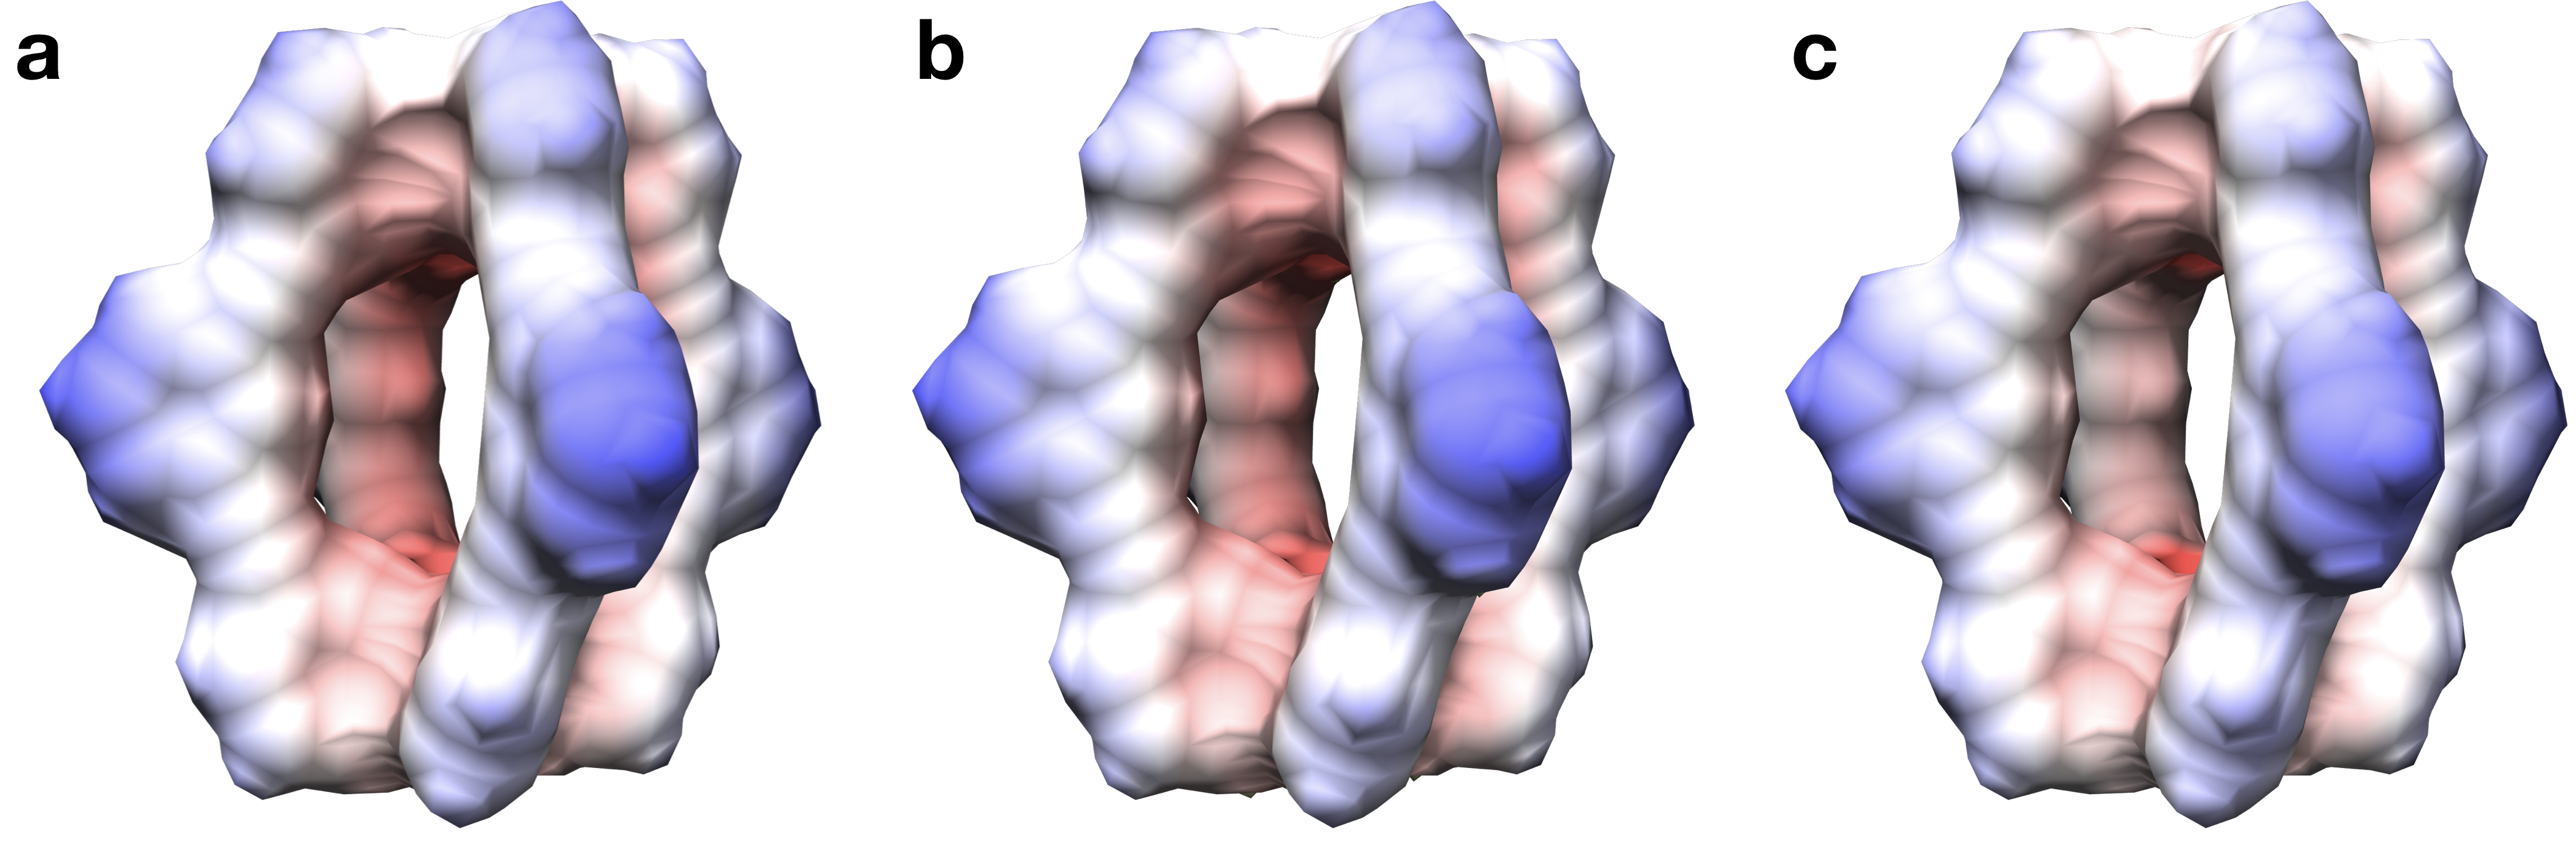
\includegraphics[width=\textwidth]{3/cgbind/figs/figS1}
	\vspace{0.2cm}
	\hrule
	\caption{Electrostatic potential plotted on the van der Waals surface using Chimera for the metallocage reported in ref. \cite{August2016}, using a uniform grid over the whole structure evaluated using (a) partial atomic charges from GFN-XTB, (b) electron density from GFN-XTB with the in-built ESP generation and (c) Multiwfn calculated ESP from a PBE/def2-SVP electron density. All geometries are identical. (a) and (b) are plotted an identical colour gradient while for (c) the full electron calculation the ESP range is not identical.}
	\label{fig::si_cg_1}
\end{figure}


\begin{figure}[h!]
	\vspace{0.4cm}
	\centering
	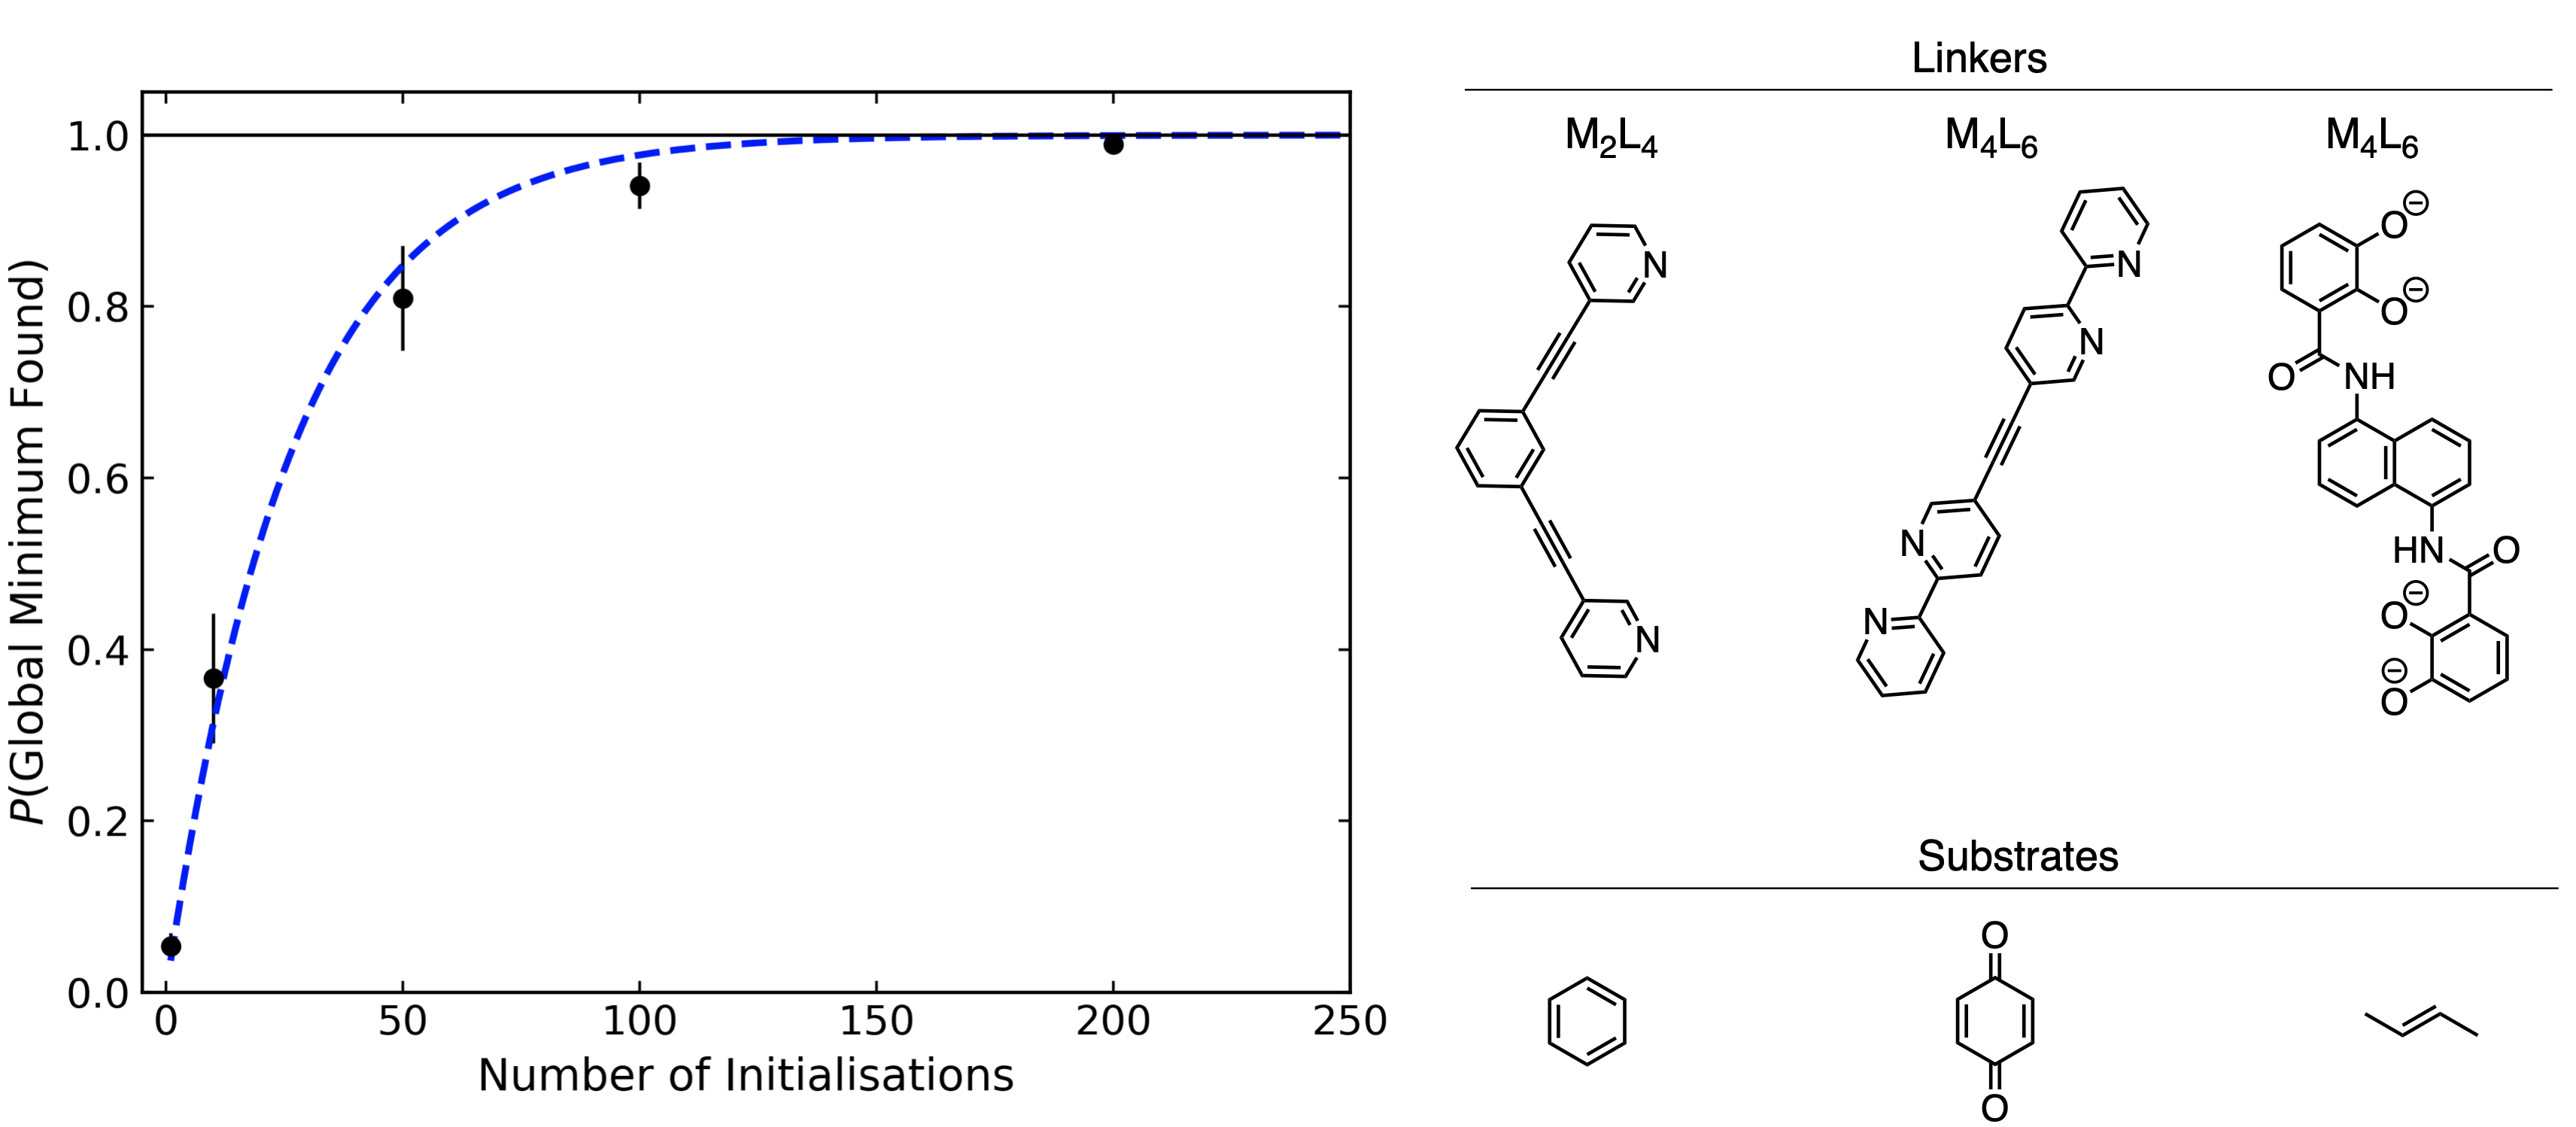
\includegraphics[width=\textwidth]{3/cgbind/figs/figS2}
	\vspace{0.2cm}
	\hrule
	\caption{Probability of locating the global minimum on the rigid body cage-substrate PES as a function of the number of random initializations for the substrate rotation matrix. Error bars correspond to the standard error in the mean for nine cage-substrate complexes generated from the linkers and substrates shown. Probabilities are determined from 500 repeats. Energy threshold between the obtained binding energy and the true global minimum was set at 0.01 \kcal.}
	\label{fig::si_cg_2}
\end{figure}



\begin{figure}[h!]
	\vspace{0.4cm}
	\centering
	 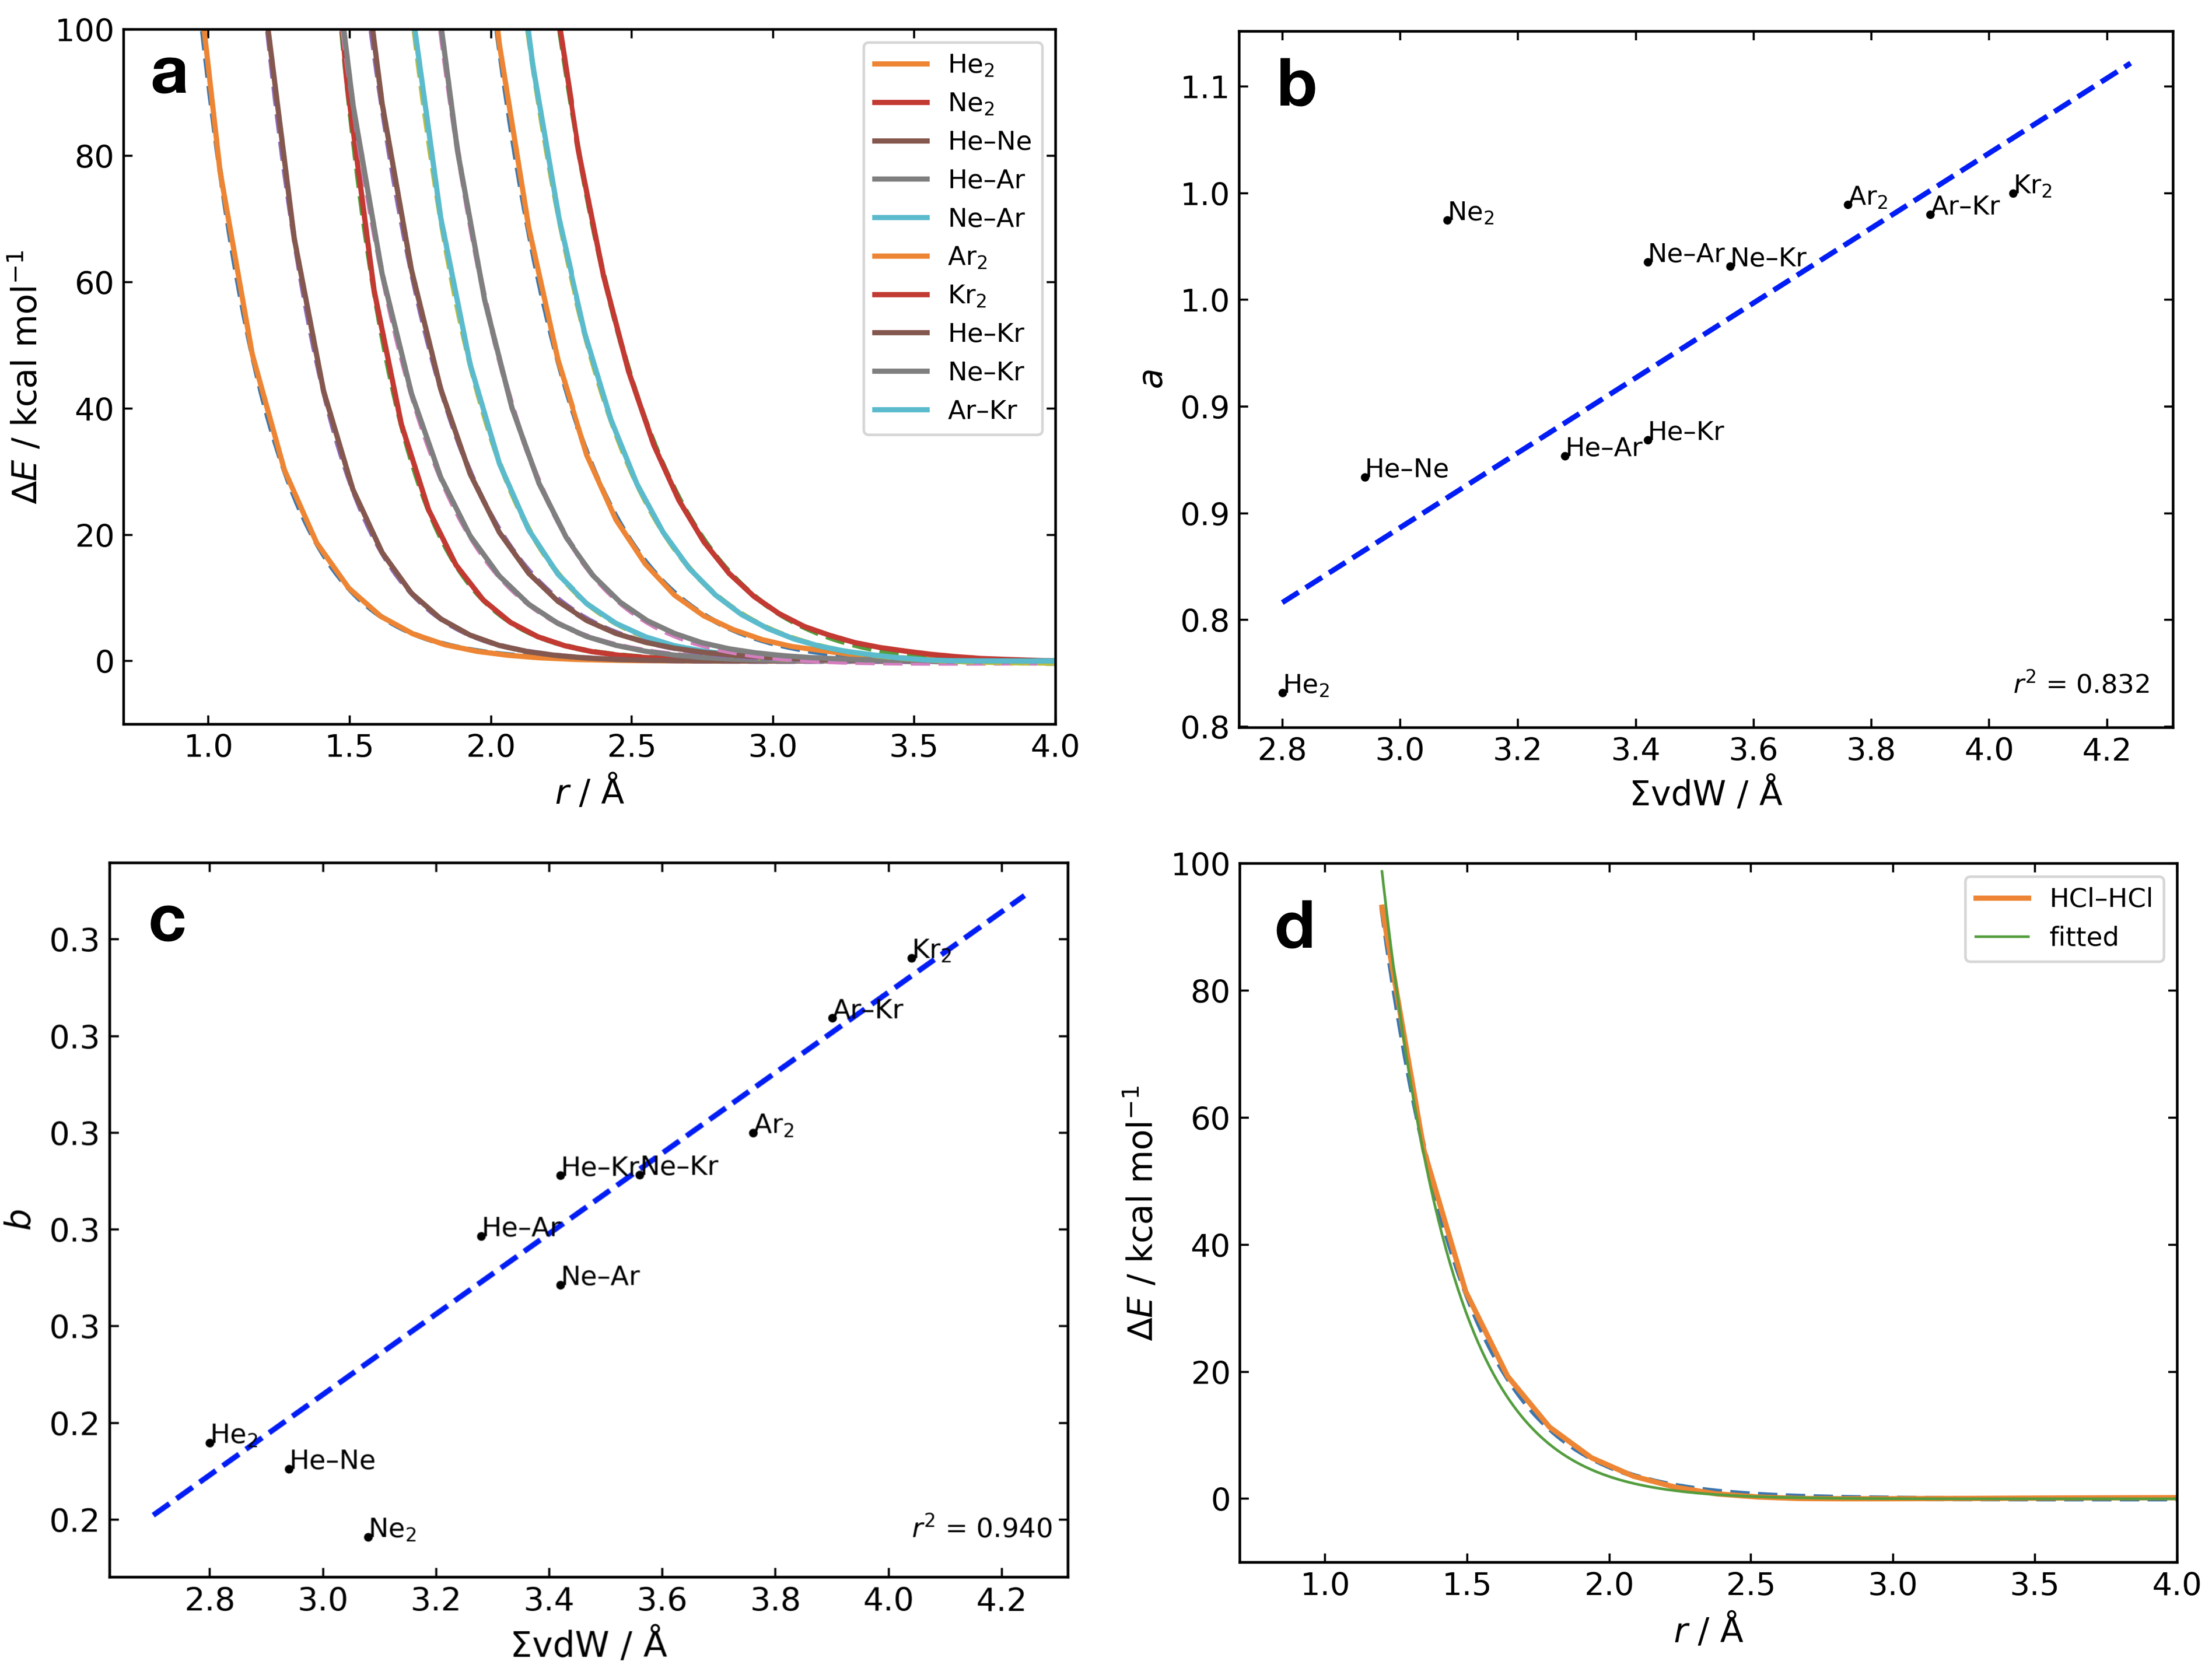
\includegraphics[width=\textwidth]{3/cgbind/figs/figS3}
	\vspace{0.2cm}
	\hrule
	\caption{(a) Noble gas dimer potential energy surfaces calculated at DLPNO-CCSD(T)/ma-def2-QZVPP in ORCA (solid lines) and fit to $V(r) = \exp(a-r/b) - c/r^6$ with Scipy (dashed lines). a, b as a function of the sum of van der Waals radii (b, c). Ne dimer excluded from the fits. a is normalized to its maximum value (aKr2). Van der Waals radii taken from ref. \cite{Mantina2009}. (d) HCl–HCl head-to-tail PES calculated as (a), d(H–Cl) = 1.27 \AA. Fitted potential (green) corresponds to a, b interpolated from the linear fits (b, c) where $\sum$vdW = 2.95 \AA$\;$ and c = 32 \kcal.}
	\label{fig::si_cg_3}
\end{figure}


\begin{figure}[h!]
	\vspace{0.4cm}
	\centering
	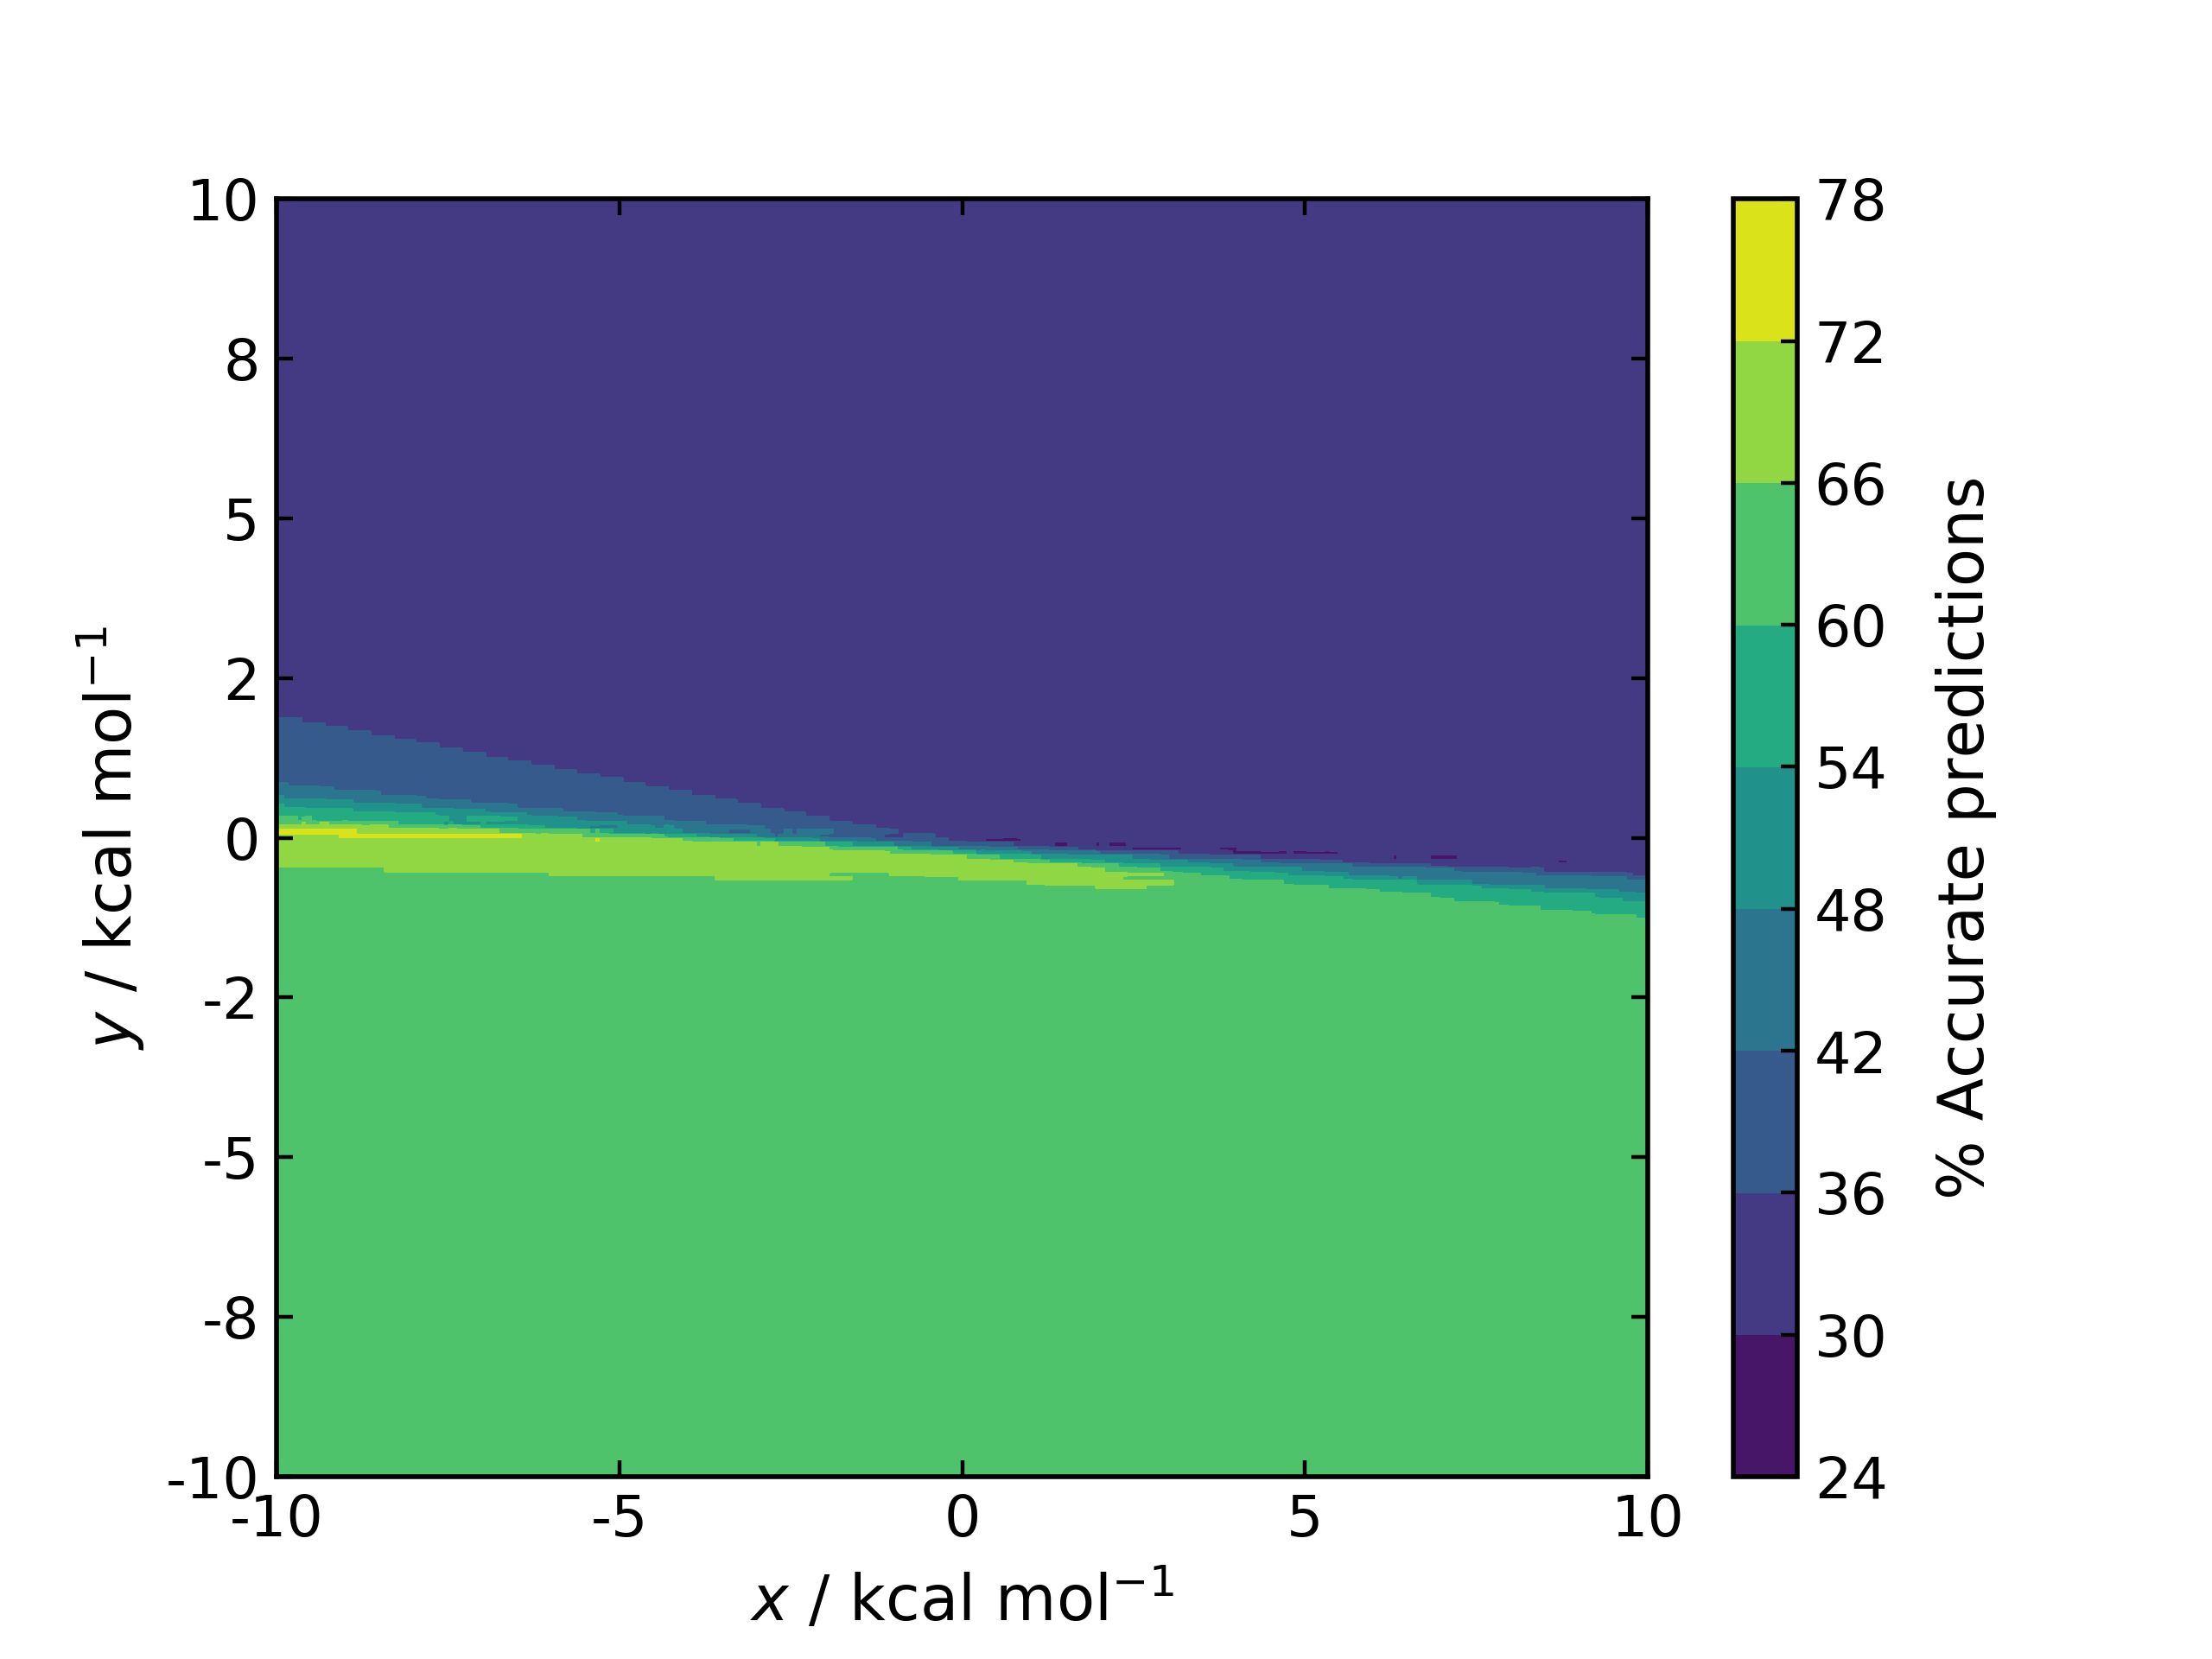
\includegraphics[width=11cm]{3/cgbind/figs/figS4}
	\vspace{0.2cm}
	\hrule
	\caption{Accuracy on prediction of 102 experimental binding affinities as a function of total binding affinity. $\text{BA}_t = \text{BA}_r + y \times$ number substrate atoms + $x$. Repulsive binding affinity $\text{BA}_r = \sum_{i>j} c \times \exp(a(i, j) - r_{ij}/b(i, j))$ where $a(i, j)$ = 11.576415 $\times$ (0.175541 $\times$ ($\gamma$i + $\gamma$j) + 0.316642), $b(i, j)$ = 0.083214 $\times$ ($\gamma$i + $\gamma$j) - 0.003768, as determined in Figure \ref{fig::si_cg_2}, $c = 1$ \kcal, $\gamma$i is the van der Waals radius of atom $i$. An accurate prediction is made if a substrate expt. binds and $\text{BA}_{t} < 0$ or expt. does not bind and $\text{BA}_ > 0$. $x$ and $y$ are plotted on a grid of 500 × 500.}
	\label{fig::sicg_4}
\end{figure}


\begin{figure}[h!]
	\vspace{0.4cm}
	\centering
	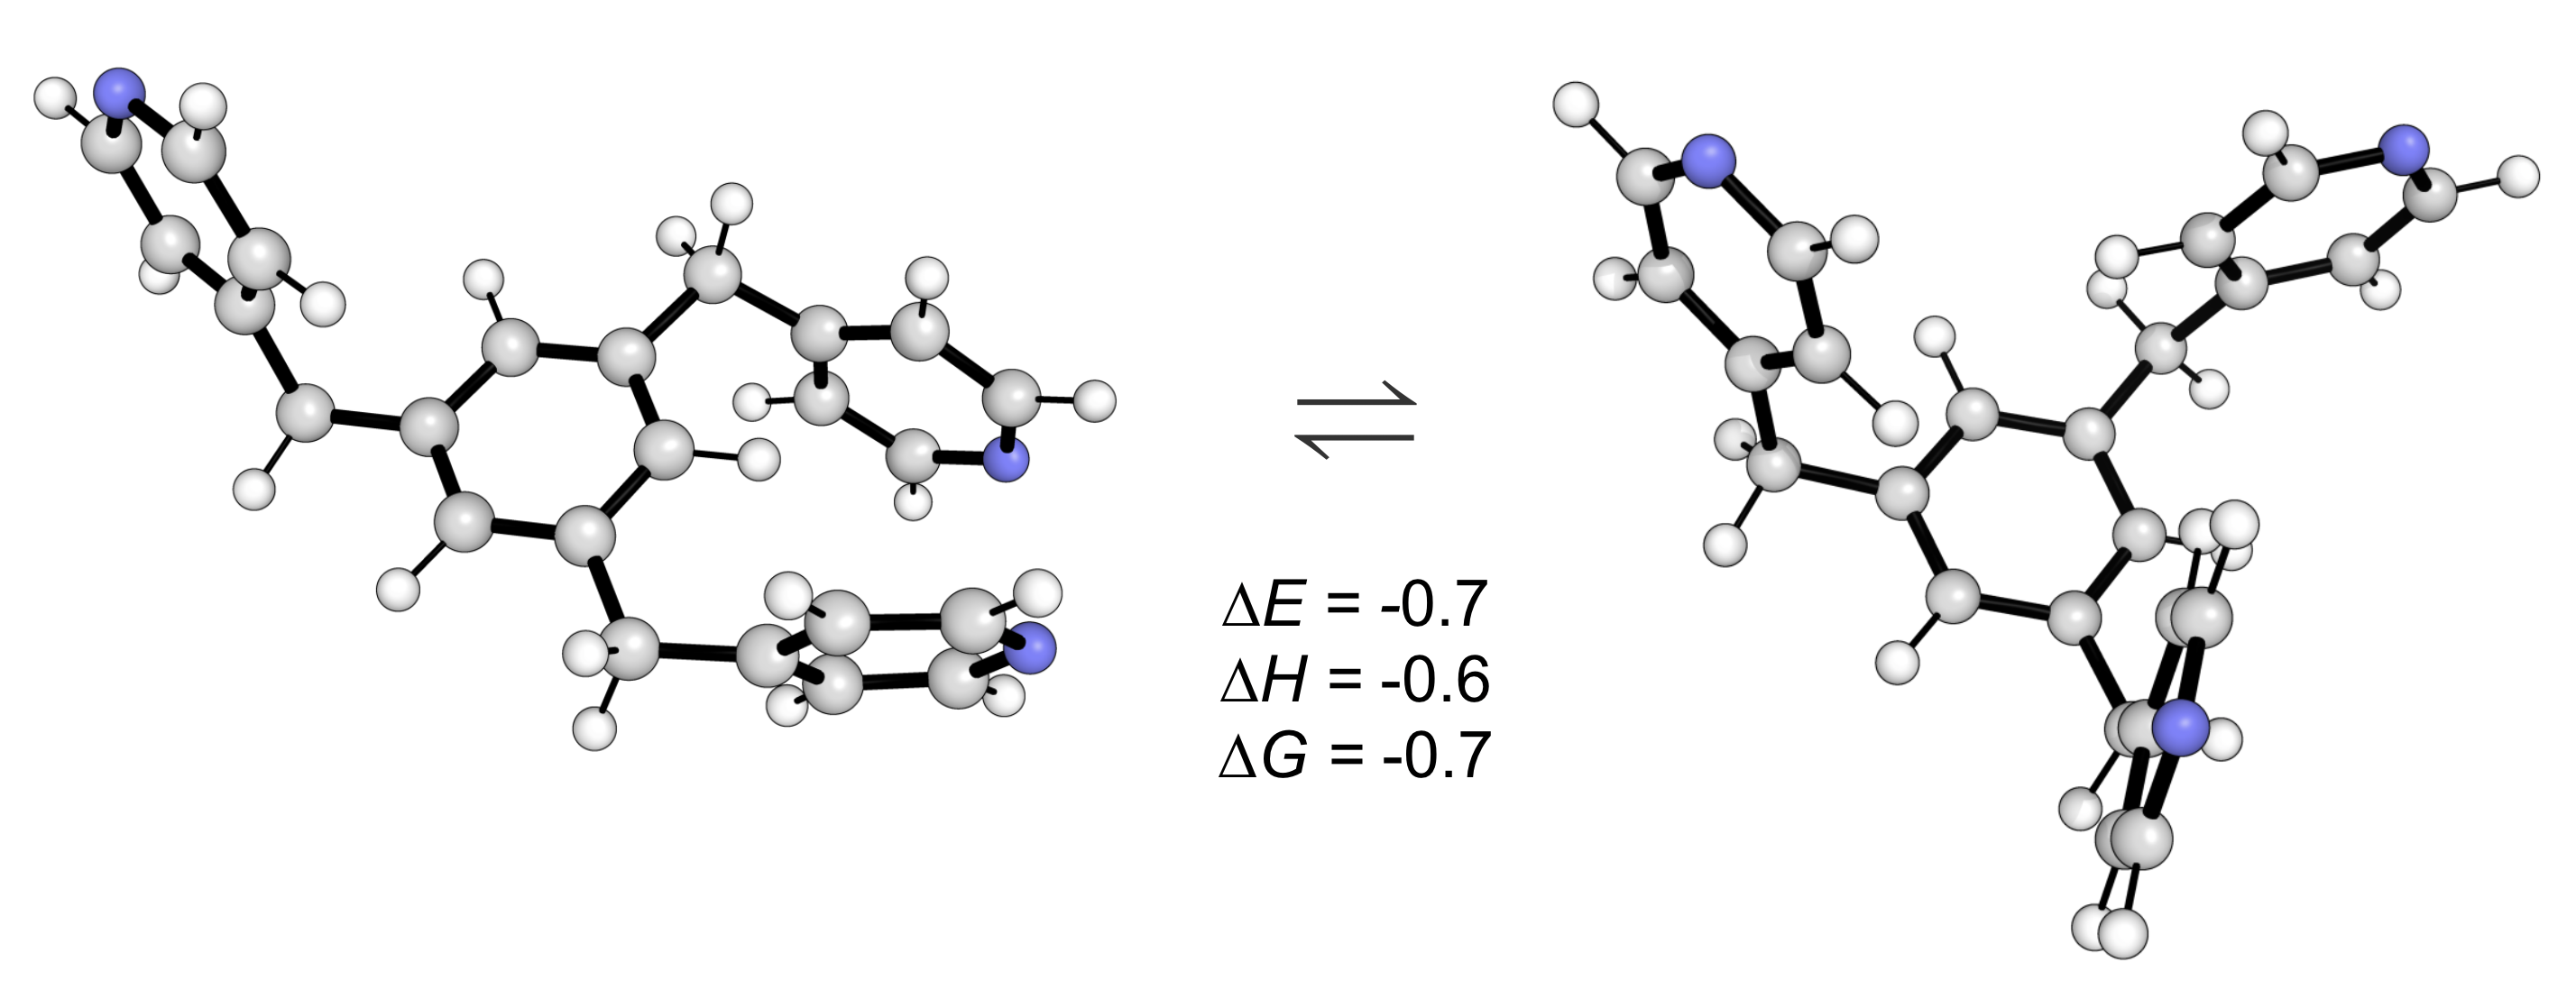
\includegraphics[width=13cm]{3/cgbind/figs/figS5}
	\vspace{0.2cm}
	\hrule
	\caption{Selected conformers of L$_h$ optimized at the PBE0-D3BJ/def2-SVP level of theory and single points calculated at DLPNO-CCSD(T)/def2-TZVPP. Frequencies were calculated to confirm that both correspond to minima (no imaginary frequencies). Energies quoted in \kcal.}
	\label{fig::si_cg_5}
\end{figure}


\begin{figure}[h!]
	\vspace{0.4cm}
	\centering
	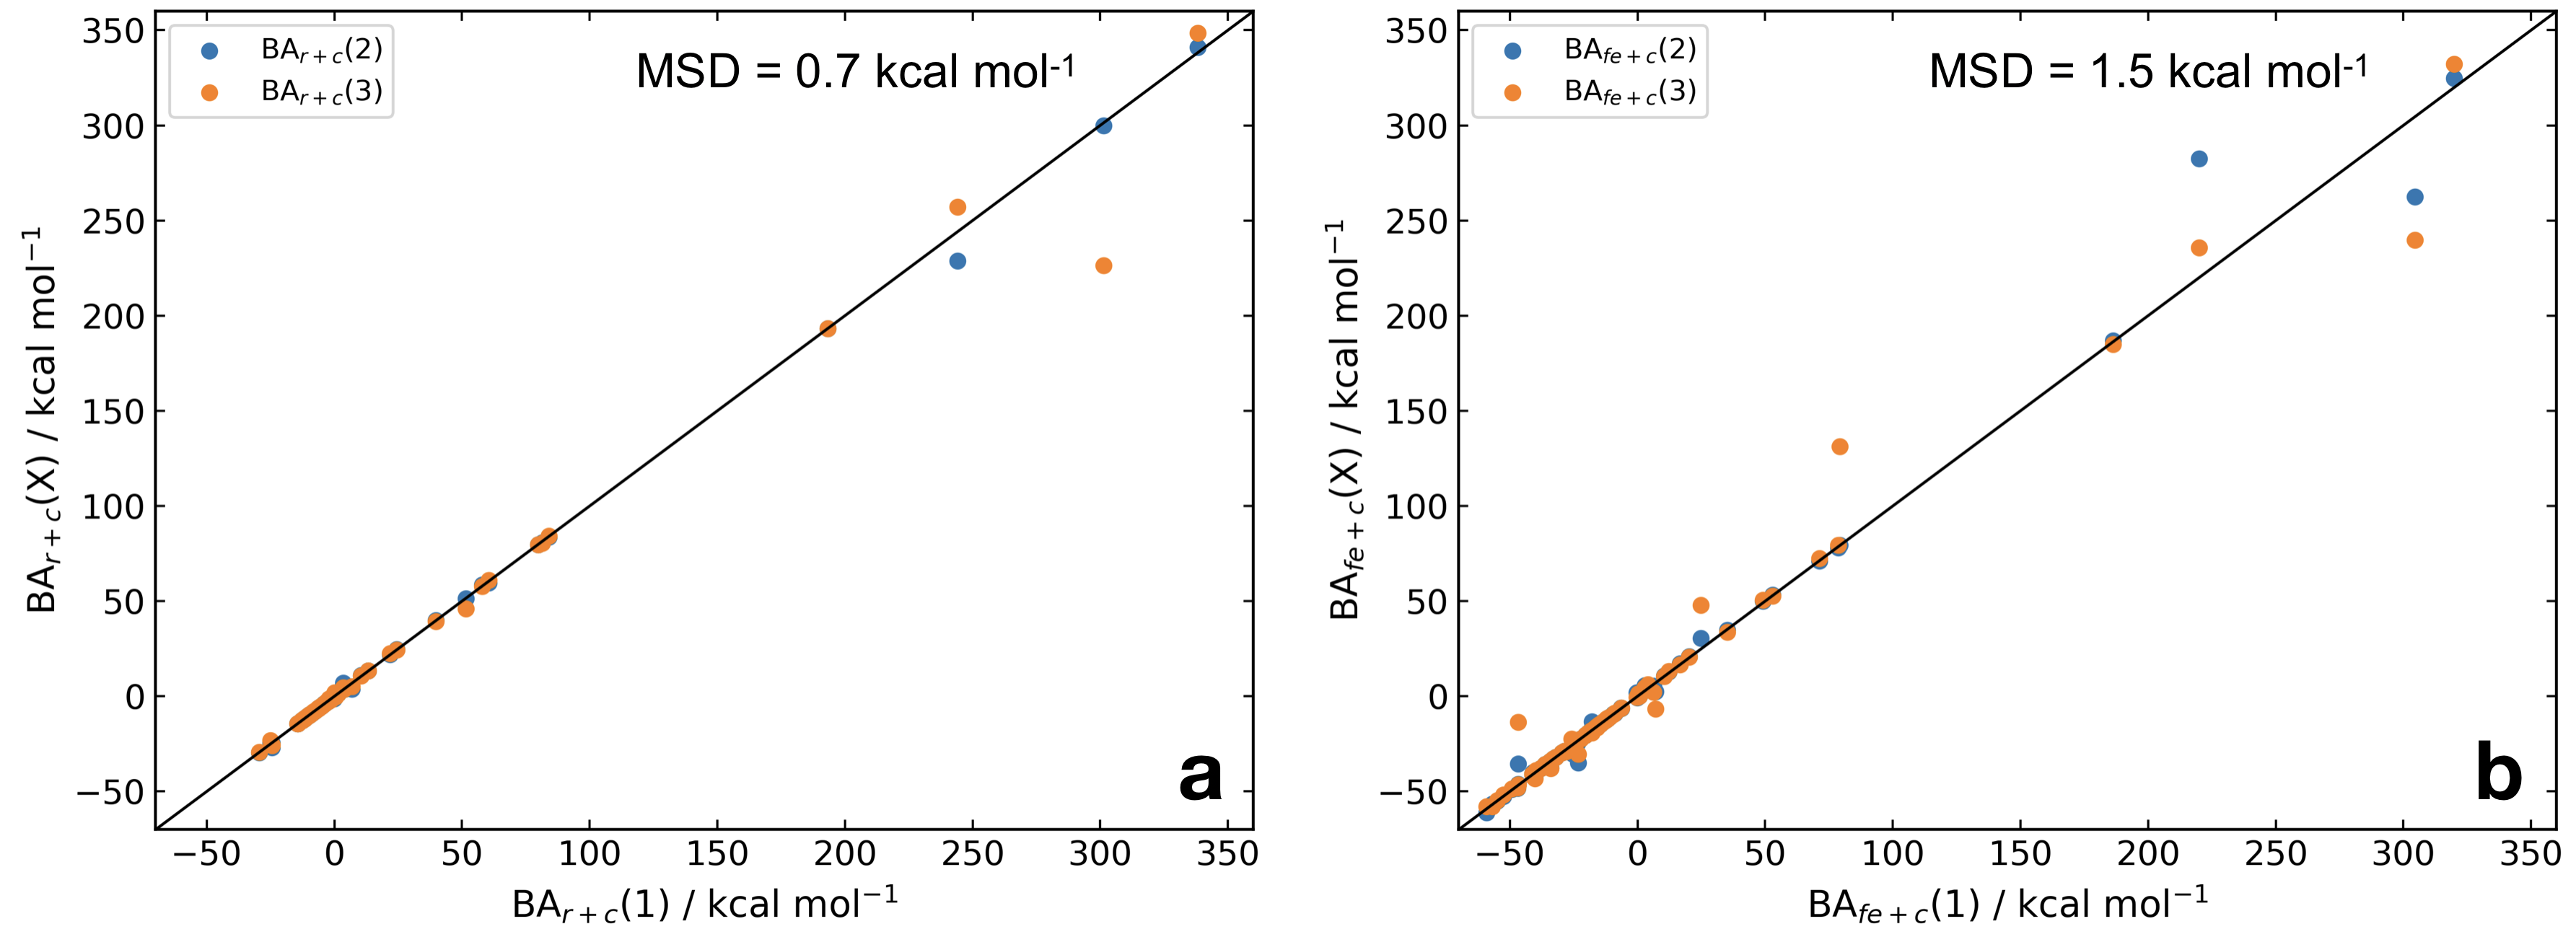
\includegraphics[width=\textwidth]{3/cgbind/figs/figS6}
	\vspace{0.2cm}
	\hrule
	\caption{Statistical error for binding affinities obtained using 3 repeats with (a) repulsive including a constant attractive term $E_\text{int}$(r+k) and (b) fast electrostatic ($E_\text{int}$(fe) methods for determining binding affinities. Mean signed deviations (MSD) are shown.}
	\label{fig::si_cg_6}
\end{figure}



\begin{figure}[h!]
	\vspace{0.4cm}
	\centering
	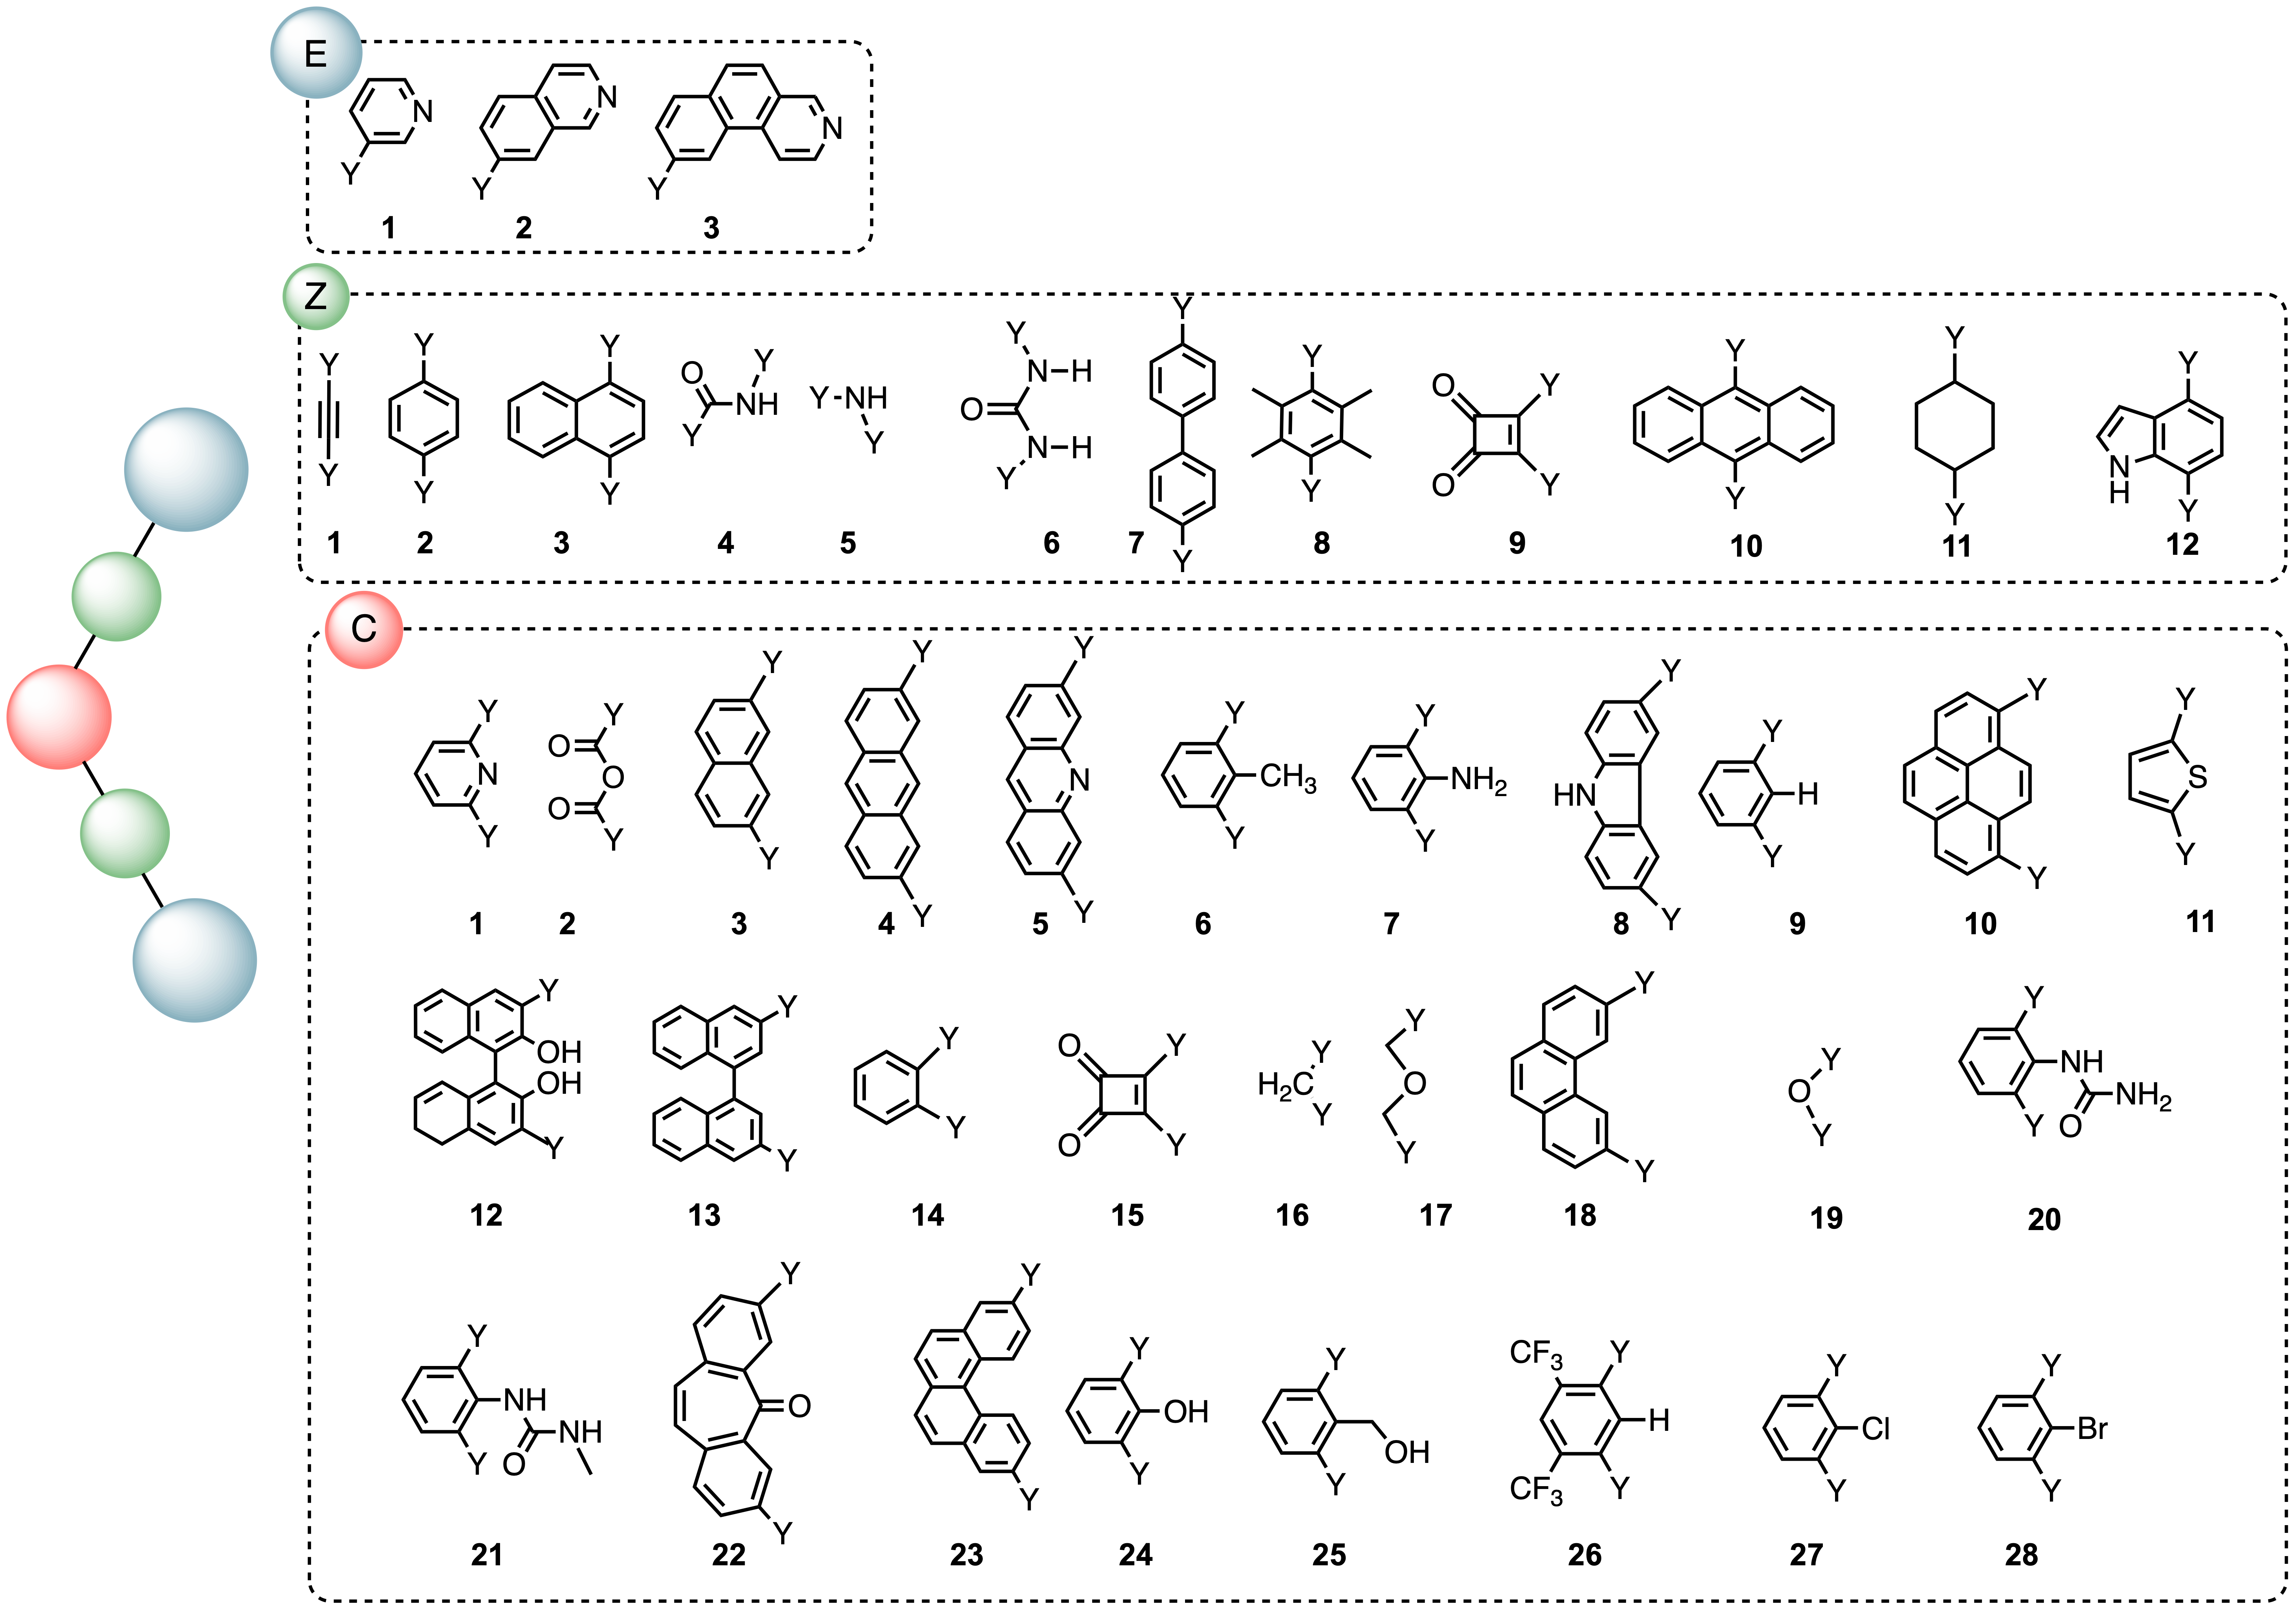
\includegraphics[width=\textwidth]{3/cgbind/figs/figS7}
	\vspace{0.2cm}
	\hrule
	\caption{Building blocks used to generate the \MLf metallocage library. Link atoms are represented by a bond to Y.}
	\label{fig::si_cg_7}
\end{figure}



\begin{table}[h!]
	\def\arraystretch{1.5}
	\begin{tabularx}{\textwidth}{YYYYYY}
		\hline
		Linker&	Cage&	Metal ion&	cgbind&	GFN-XTB//cgbind&PBE-D3BJ/def2-SVP//cgbind\\
		\hline
		La	&a$^{a,b}$&	Pd(II)&	0.45559	&0.41474	&0.46321
\\
		Lb	&b			&	Pd(II)&	0.79541	&0.91896	&1.76651
\\
		Lc	&c$^{b}$&	Pd(II)&	0.62754	&0.47084&	0.47219
\\
		Ld	&d$^{a,b}$&	Fe(III)	&1.37837&	2.01894	&2.84652
\\
		Le&	e		&			Mn(II)&	0.82032	&0.25010&	0.67427
\\
		Lf&	f				&	Fe(II)	&1.09910&	0.73566	&1.17804
\\
		Lg	&g$^{a}$	&	Pd(II)&	1.29529	&1.73599&	1.98475
\\
		Lh	&h$^{b,c}$	&	Pd(II)&	1.21209	&0.47521&	0.68496
\\
		Li&	i$^{b}$			&Cu(II)&	1.40281	&2.05635	&1.76552
\\
		
	\end{tabularx}
	\hrule
	\caption{Root mean squared displacements (\AA) to crystal structures of \cgbind generated geometries and subsequent optimisations with tight-binding and standard DFT. $a.$ Crystal structure used to generate the template. b. Unmodified crystal structure contains encapsulated molecule(s). c. Conformer generated manually. n.c: Not calculated.}
	\label{table::si_cg_1}
\end{table}



\begin{figure}[h!]
	\vspace{0.4cm}
	\centering
	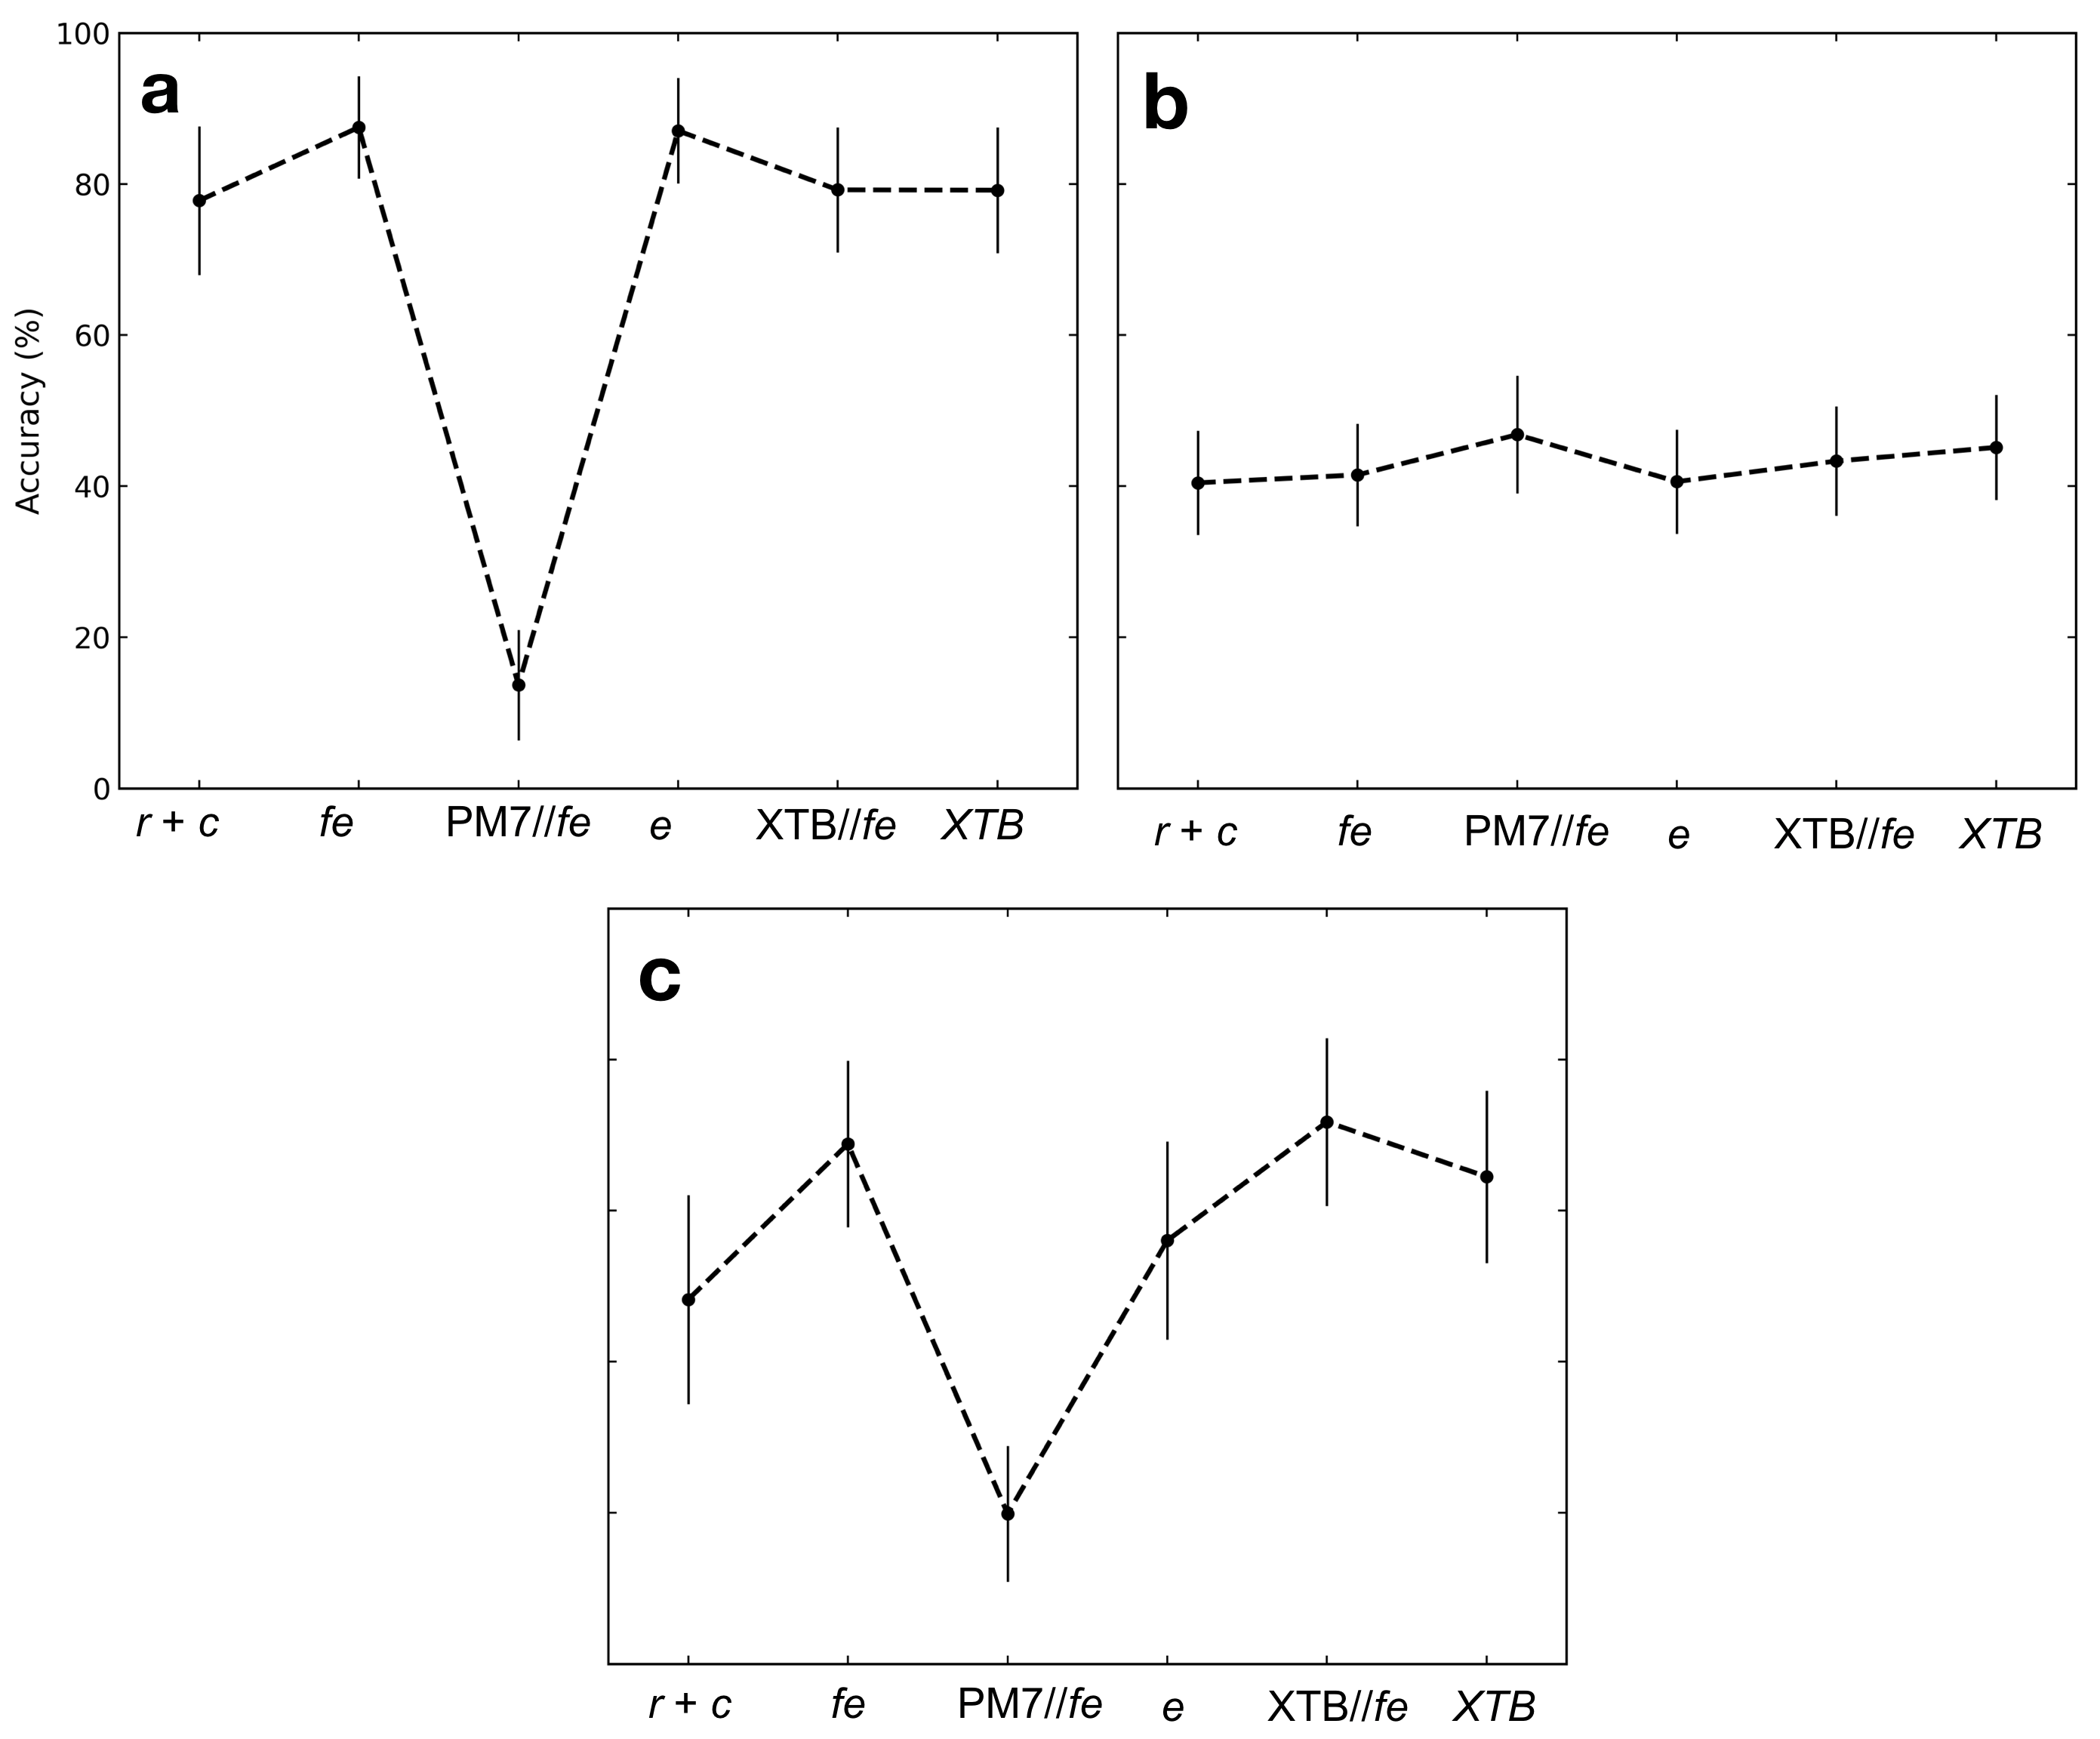
\includegraphics[width=\textwidth]{3/cgbind/figs/figS8.png}
	\vspace{0.2cm}
	\hrule
	\caption{Binding affinity predictions for (a) 24 host-guest complexes with two different Pd(II)$_2$L$_4$ cages refs. \cite{August2016} and \cite{MartCentelles2018}; (b) 54 hots-guest complexes with a series of aromatic-panelled Fe(II)$_4$L$_6$  tetrahedral cages ref. \cite{Ronson2017}; (c) 24 host-guest complexes with Fe(II)$_4$L$_6$ tetrahedral cages (ref. \cite{Smulders2013}).}
	\label{fig::si_cg_8}
\end{figure}




\begin{figure}[h!]
	\vspace{0.4cm}
	\centering
	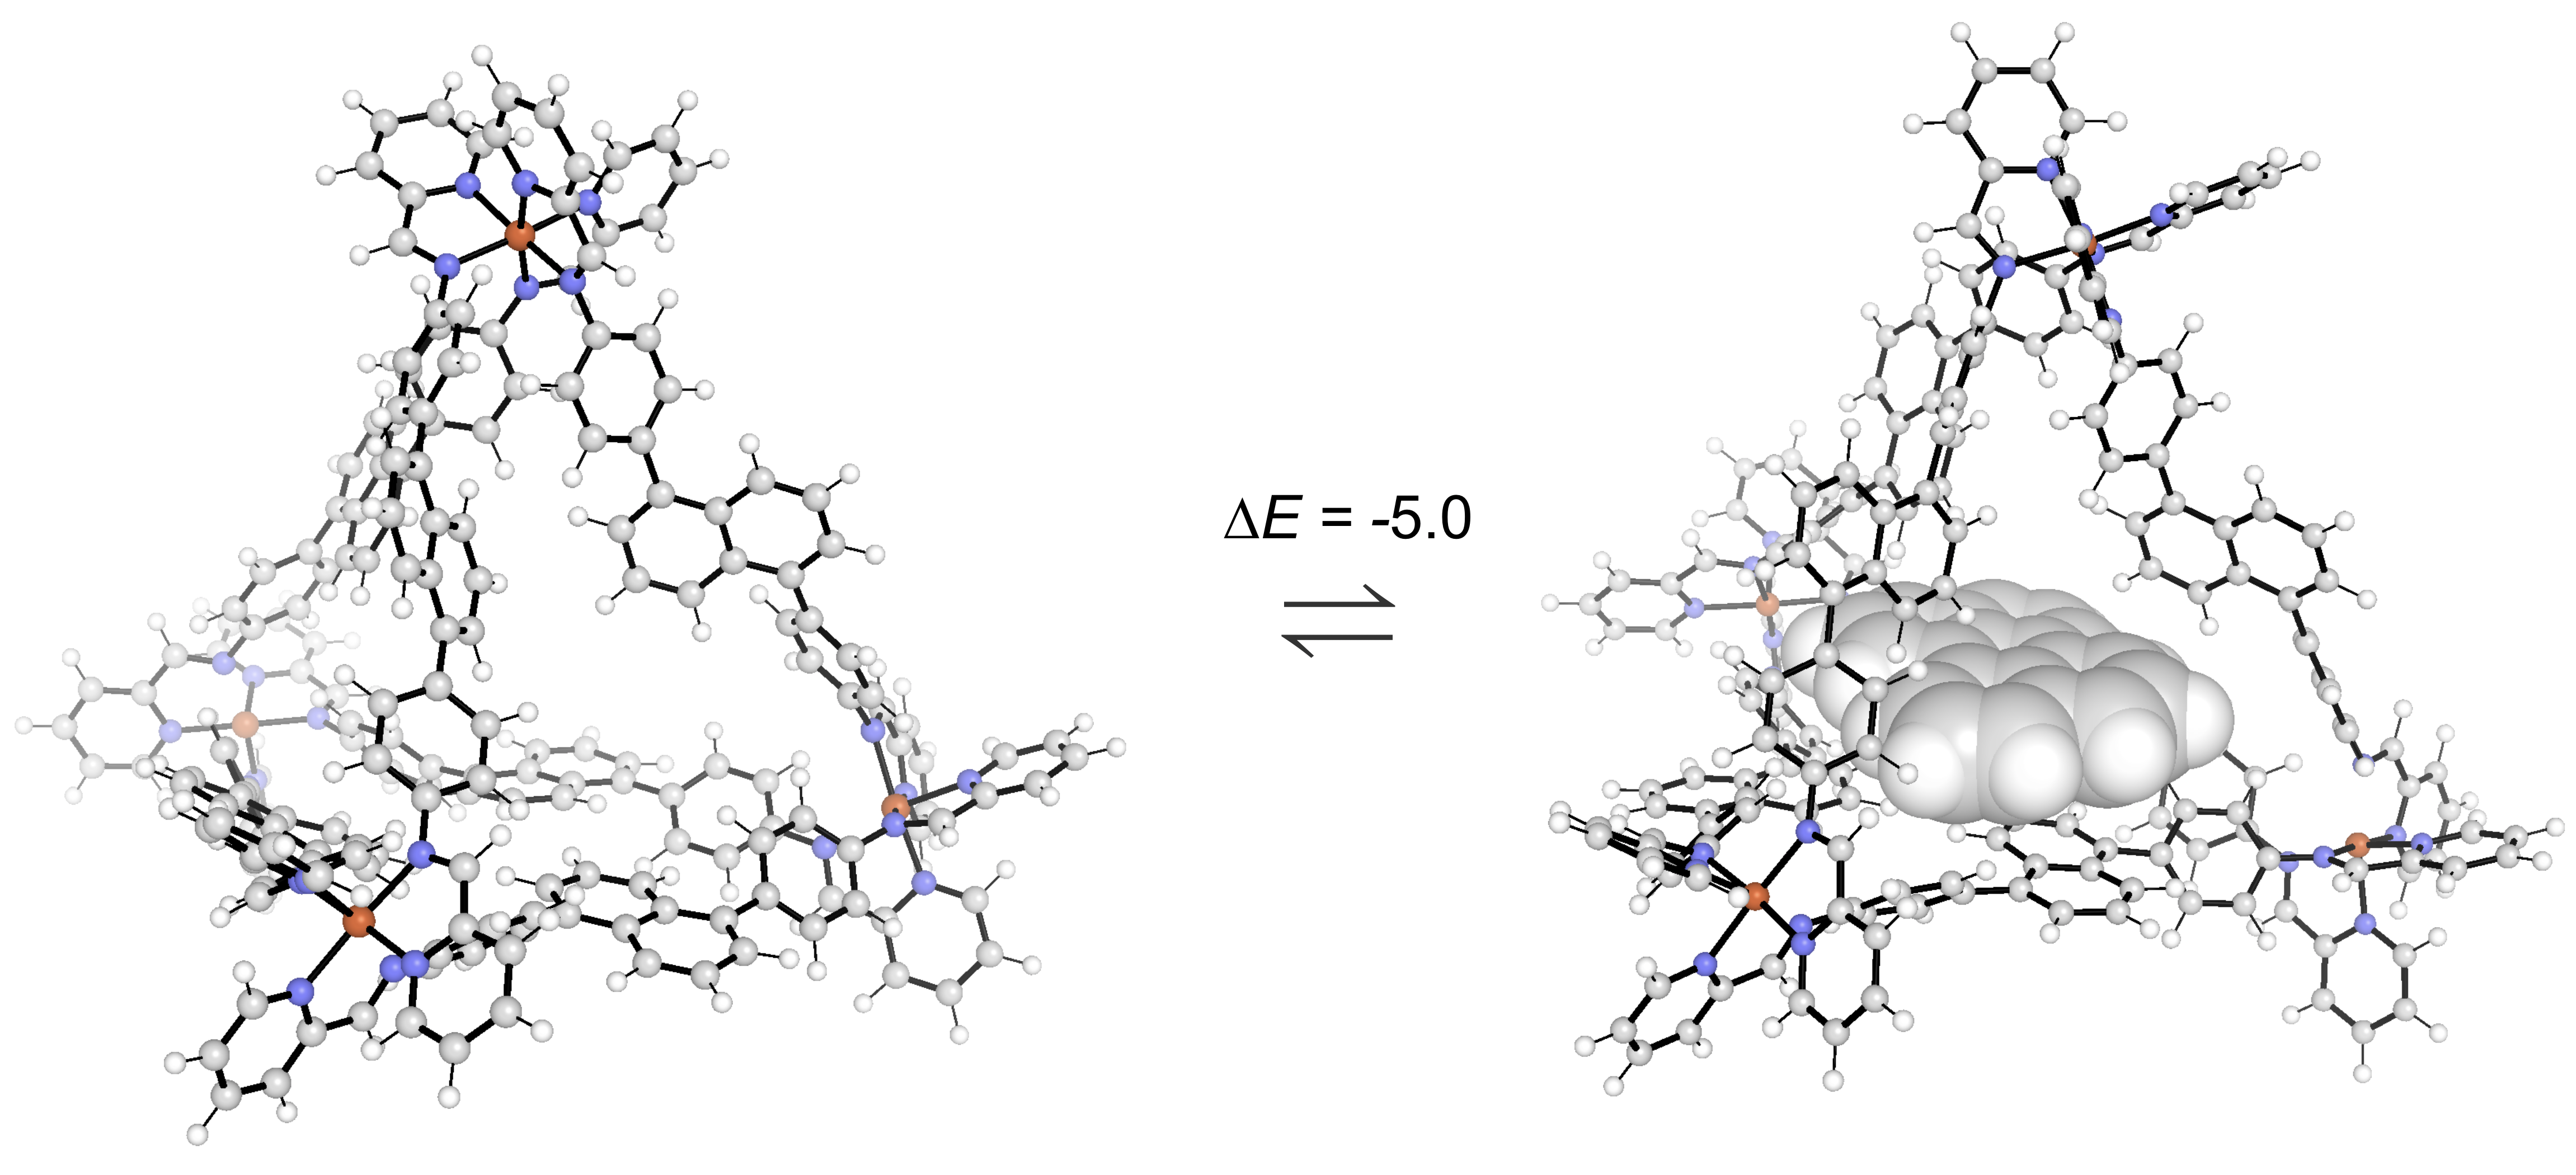
\includegraphics[width=\textwidth]{3/cgbind/figs/figS9}
	\vspace{0.2cm}
	\hrule
	\caption{DFT optimized structures of cage (C-42) and cage-substrate complex (CS-42) and the binding affinity (\de$\;$ in \kcal) is computed at the SMD(MeCN)-M06-2X/def2-TZVP//PBE-D3BJ/def2-SVP level of theory. Due to the large molecular size the geometry optimization of C-42 and CS-42 were converged with respect to binding affinity (\dde $\;< 1$ \kcal).}
	\label{fig::si_cg_9}
\end{figure}


\clearpage
\end{document}